\noindent In Kapitel 3 werden die grafische Darstellung von Datens\"{a}tzen und die zusammenfassende Beschreibung der Daten durch Lage- und Streuungskennwerte eingef\"{u}hrt. Diese Daten k\"{o}nnen als Stichprobe einer Grundgesamtheit verstanden werden. In diesem Kapitel werden Schl\"{u}sse aus einer Stichprobe f\"{u}r die zugeh\"{o}rige Grundgesamtheit gezogen. Insbesondere werden auf Basis einer Stichprobe Parameter der Grundgesamtheit gesch\"{a}tzt und der Bereich f\"{u}r zuk\"{u}nftige Werte prognostiziert.


\subsection{Zielsetzung und Problematik der Parametersch\"{a}tzung}

\noindent Im Rahmen der Design For Six Sigma Methoden werden Mittelwert $\mu$ und Standardabweichung $\sigma$ einer Verteilung auf Basis des Mittelwertes $\overline{\mathrm{x}}$ und der Standardabweichung s der Stichprobe gesch\"{a}tzt. Der Stichprobenmittelwert ist der Sch\"{a}tzwert f\"{u}r den Mittelwert der Grundgesamtheit. 

\begin{equation}\label{eq:fiveone}
\mu \approx \bar{x}
\end{equation}

\noindent In gleicher Weise wird die Stichprobenvarianz als Sch\"{a}tzwert f\"{u}r die Varianz der Grundgesamtheit verwendet.

\begin{equation}\label{eq:fivetwo}
\sigma ^{2} \approx s^{2}
\end{equation}

\begin{table}[H]
\setlength{\arrayrulewidth}{.1em}
\caption{Sch\"{a}tzung der Parameter einer Grundgesamtheit \"{u}ber eine Stichprobe}
\setlength{\fboxsep}{0pt}%
\colorbox{lightgray}{%
\arrayrulecolor{white}%
\begin{tabular}{| wc{4cm} | wc{6cm} | wc{6cm} }
\xrowht{20pt}

{\fontfamily{phv}\selectfont\textbf{Charakteristik}} & 
{\fontfamily{phv}\selectfont\textbf{Stichprobe}} &
{\fontfamily{phv}\selectfont\textbf{Grundgesamtheit}}\\ \hline \xrowht{20pt}

\multirow{2}{*}{\fontfamily{phv}\selectfont{Mittelwert}} &
{\fontfamily{phv}\selectfont{$\bar{x}$}} & 
{\fontfamily{phv}\selectfont{$\nu$}} \\ \cline{2-3} \xrowht{20pt}
& \multicolumn{2}{c}{\fontfamily{phv}\selectfont{Stichproben-Mittelwert $\bar{x}$ schätzt den Mittelwert der Grundgesamtheit $\nu$}} \\ \hline \xrowht{20pt}

\multirow{2}{*}{\fontfamily{phv}\selectfont{Varianz}} &
{\fontfamily{phv}\selectfont{$s^{2}$}} & 
{\fontfamily{phv}\selectfont{$\sigma ^{2} $}} \\ \cline{2-3} \xrowht{20pt}
& \multicolumn{2}{c}{\fontfamily{phv}\selectfont{Stichproben-Varianz s$^{2}$ sch\"{a}tzt die Varianz der Grundgesamtheit $\sigma^{2}$}} \\ \hline

\end{tabular}%
}\bigskip
\label{tab:fiveone}
\end{table}

\noindent Tabelle \ref{tab:fiveone} stellt den Zusammenhang zwischen Grundgesamtheit und Stichprobe tabellarisch zusammen.

\noindent Mit den gesch\"{a}tzten Parametern ergibt sich eine Verteilung der Grundgesamtheit. Bild \ref{fig:StichprobenSchaetzungMotivation1} verbindet die als Stabdiagramm dargestellte Stichprobe und die gesch\"{a}tzte Wahrscheinlichkeitsdichte der Grundgesamtheit.

\noindent 
\begin{figure}[H]
  \centerline{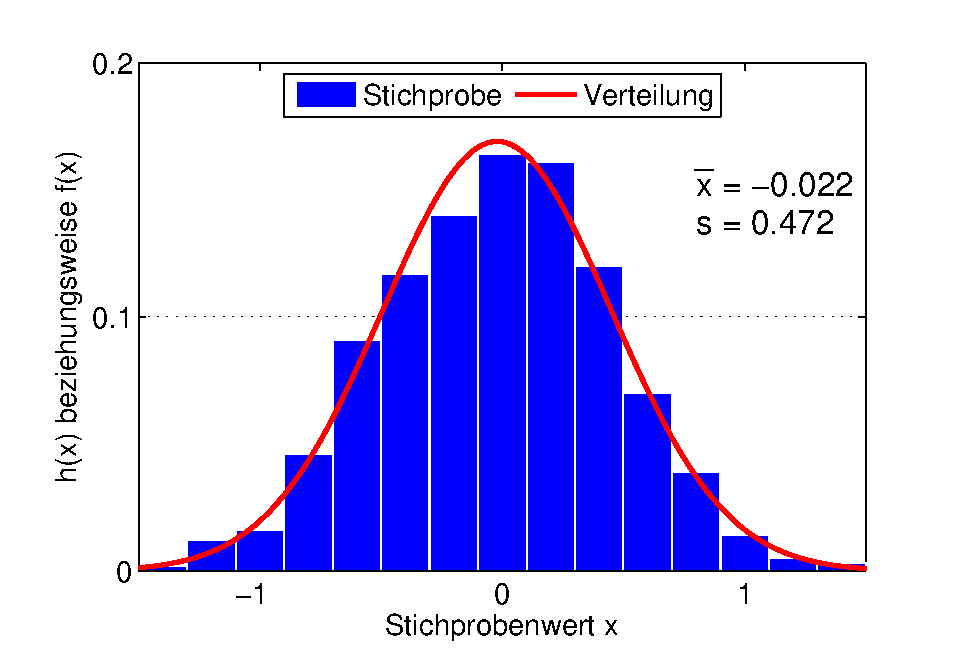
\includegraphics[width=0.5\textwidth]{Kapitel5/Bilder/image1}}
  \caption{Stichprobe und auf Basis der Stichprobe gesch\"{a}tzte Wahrscheinlichkeitsdichte der Grundgesamtheit}
  \label{fig:StichprobenSchaetzungMotivation1}
\end{figure}

\noindent Um die Problematik der beurteilenden Statistik zu verdeutlichen, wird eine Stichprobe aus einem Datensatz analysiert, der eine normalverteilte Grundgesamtheit mit einem Mittelwert von $\mu$ = 0 und einer Standardabweichung von $\sigma$ = 0.5 aufweist. Bild \ref{fig:StichprobenSchaetzungMotivation2} zeigt die relativen H\"{a}ufigkeiten zweier Stichproben mit einem Umfang von jeweils 10 Werten.

\noindent 
\begin{figure}[H]
  \centerline{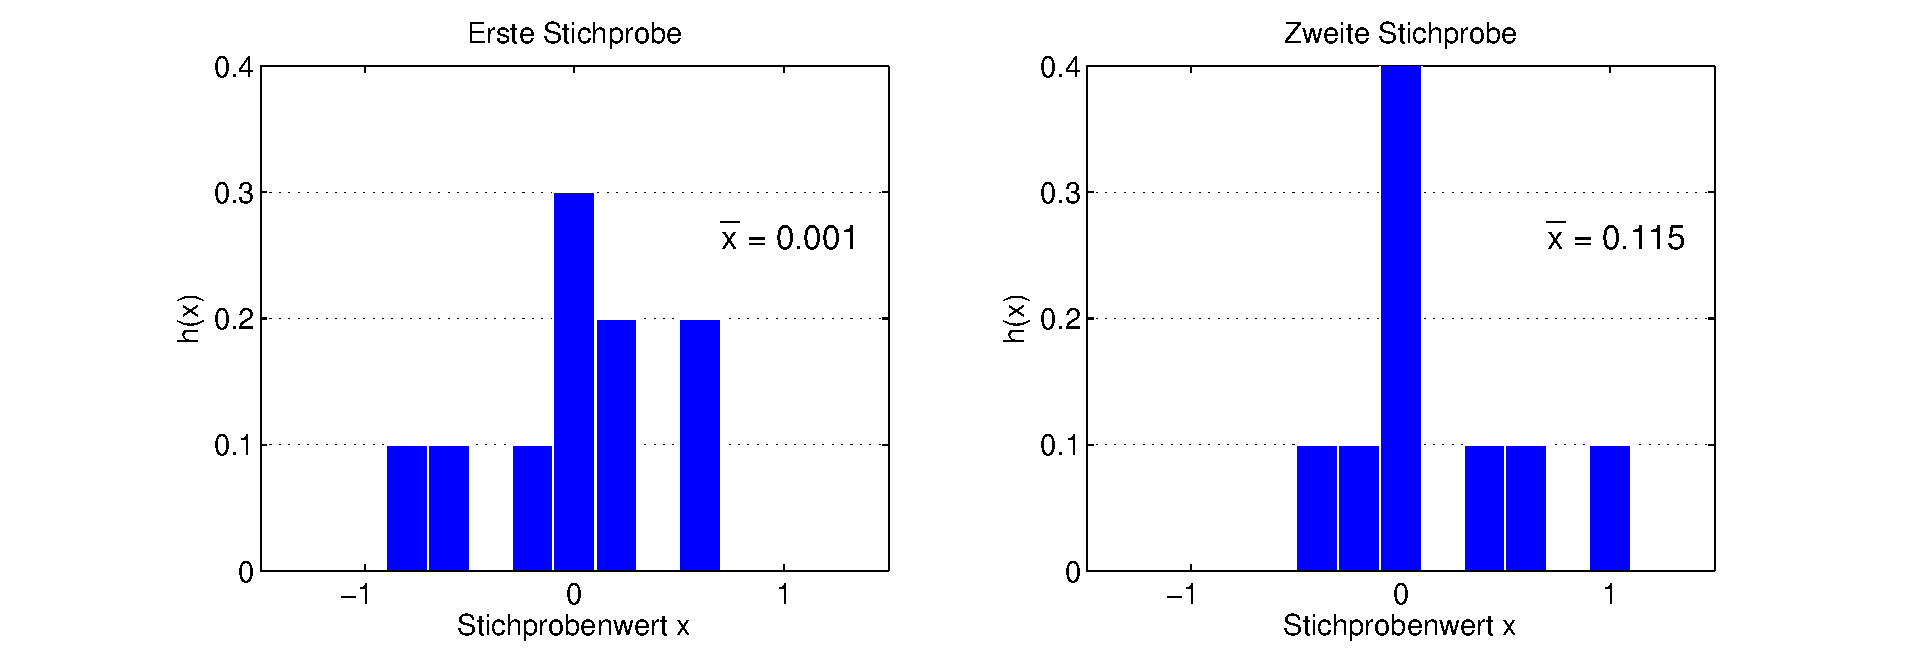
\includegraphics[width=1\textwidth]{Kapitel5/Bilder/image2}}
  \caption{H\"{a}ufigkeitsverteilungen zweier unterschiedlicher Stichproben derselben Grundgesamtheit mit einem Stichprobenumfang von N = 10}
  \label{fig:StichprobenSchaetzungMotivation2}
\end{figure}

\noindent Obwohl die beiden Stichproben mit dem Umfang von 10 Teilen aus derselben Grundgesamtheit stammen, weichen ihre Mittelwerte $\overline{\mathrm{x}}$ stark voneinander ab. Das Beispiel zeigt, dass der Mittelwert der Grundgesamtheit auf Basis einer Stichprobe nur gesch\"{a}tzt werden kann. Er h\"{a}ngt von der Auswahl der Stichprobenwerte ab. Der \"{u}ber eine Stichprobe gesch\"{a}tzte Mittelwert ist damit selber eine Zufallsgr\"{o}{\ss}e. 

\clearpage

\noindent Um den Einfluss des Stichprobenumfangs zu hinterfragen, wird auf derselben Datenbasis der Stichprobenumfang in Schritten von N = 10, 100 und 1000 Werte erweitert. Das Ergebnis ist in Bild \ref{fig:StichprobenSchaetzungMotivation3} dargestellt. 

\noindent 
\begin{figure}[H]
  \centerline{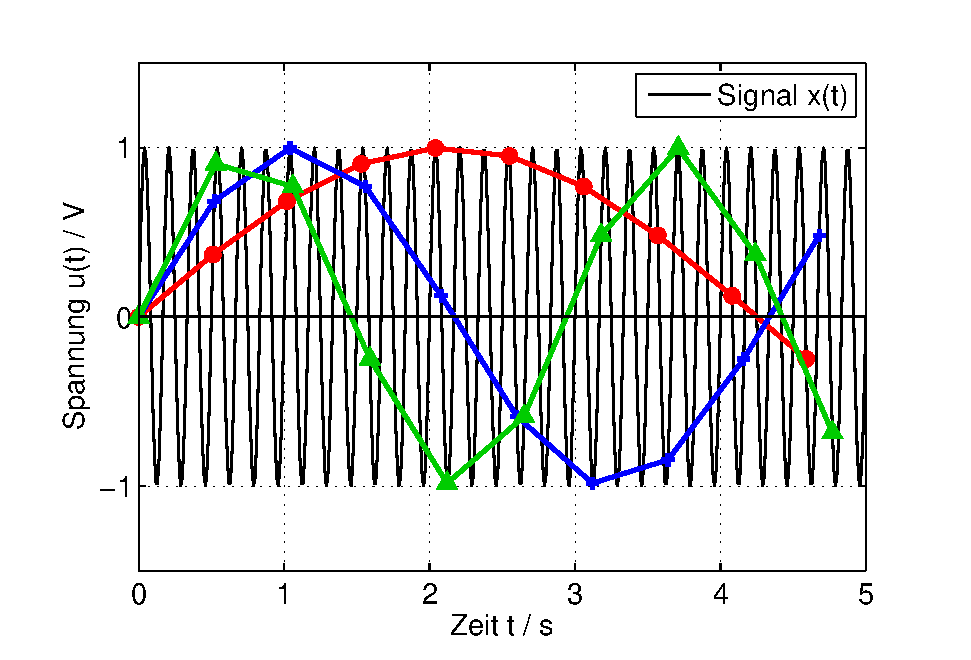
\includegraphics[width=1\textwidth]{Kapitel5/Bilder/image3}}
  \caption{H\"{a}ufigkeitsverteilungen von Stichproben derselben Grundgesamtheit mit einem Stichprobenumfang von N = 10, 100, 1000 }
  \label{fig:StichprobenSchaetzungMotivation3}
\end{figure}

\noindent Mit steigendem Stichprobenumfang n\"{a}hert sich der Mittelwert der Stichprobe $\overline{\mathrm{x}}$ dem wahren Mittelwert $\mu$ = 0 an. Die Sch\"{a}tzung des Mittelwertes wird also mit wachsendem Stichprobenumfang genauer. Aus Genauigkeitsgr\"{u}nden erscheint es deshalb erstrebenswert, m\"{o}glichst viele Stichprobenwerte zu analysieren. Allerdings sprechen finanzielle, zeitliche oder prinzipielle Gr\"{u}nde f\"{u}r einen geringen Stichprobenumfang. Damit stellt sich die Frage, wie gro{\ss} der Stichprobenumfang f\"{u}r eine bestimmte Aufgabe sein muss. Diese Frage wird mit der Bestimmung von Konfidenzintervallen beantwortet.\newline

\noindent Die Darstellung der Stichprobe mit wachsendem Stichprobenumfang in Bild \ref{fig:StichprobenSchaetzungMotivation3} verdeutlicht aber noch eine zweite Fragestellung. Bei einem geringen Stichprobenumfang ist die zugrunde liegende Verteilung nicht erkennbar. Sie ist erst bei gr\"{o}{\ss}eren Stichprobenumf\"{a}ngen zu erkennen. Eine weitere Aufgabenstellung widmet sich deshalb der Frage, wie sicher es sich bei der vorliegenden Stichprobe um eine bestimmte Verteilung handelt. Diese Frage wird in Kapitel 12 mithilfe des sogenannten Wahrscheinlichkeitsnetzes beantwortet. Die Darstellungen in diesem Kapitel beschr\"{a}nken sich auf normalverteilte Zufallsvariable.\newline

\noindent In diesem Kapitel wird die Theorie der Stichprobenentnahme aus einer unendlichen Grundgesamtheit vorgestellt. Dabei wird davon ausgegangen, dass die Wahrscheinlichkeit eines Stichprobenwertes nicht von den anderen Stichprobenwerten beeinflusst wird. Das ist insbesondere f\"{u}r eine unendlich gro{\ss}e Grundgesamtheit der Fall, woraus sich die Bezeichnung der Theorie ergibt. Praktisch gesehen wird diese Annahme aber auch dann erf\"{u}llt, wenn die Grundgesamtheit sehr viel gr\"{o}{\ss}er ist als die Anzahl der Stichproben, sodass die Annahme in nahezu allen praktischen F\"{a}llen berechtigt ist. \newline

\noindent Weiterhin werden bei den Herleitungen Rechenregeln f\"{u}r mehrere unabh\"{a}ngige Zufallsvariablen ben\"{o}tigt, die in Kapitel 8 ausf\"{u}hrlich dargestellt sind. Um Fragestellungen f\"{u}r univariate Verteilungen abschlie{\ss}en zu k\"{o}nnen, wird die Berechnung von Konfidenzbereichen vorgezogen.

\clearpage

\subsection{Erwartungstreue der Parametersch\"{a}tzung}

\noindent Die Grundgesamtheit des zu analysierenden Wahrscheinlichkeitsprozesses weist einen Mittelwert $\mu$ und eine Varianz $\sigma^{2}$ auf. Beide Kenngr\"{o}{\ss}en werden auf Basis einer Stichprobe mit den Werten x$_{1}$, x$_{2}$, ..., x$_{N}$ gesch\"{a}tzt. Dabei stellt sich die Frage, ob die gesch\"{a}tzten Parameter bei einer gro{\ss}en Anzahl von Stichprobenwerten mit dem erwarteten Parameter der Grundgesamtheit \"{u}bereinstimmen.

\subsubsection{Sch\"{a}tzen des Mittelwertes einer Grundgesamtheit}

\noindent Der Mittelwert aus einer Stichprobe x${}_{1}$, x${}_{2}$, ..., x${}_{N}$ wird als Sch\"{a}tzwert des Mittelwertes µ der Grundgesamtheit angesehen. Die Sch\"{a}tzung ergibt sich aus der Beziehung

\begin{equation}\label{eq:fivethree}
\mu \approx \bar{x}=\dfrac{1}{N} \cdot \left(x_{1} +x_{2} +...+x_{N} \right)=\dfrac{1}{N} \cdot \sum _{n=1}^{N}x_{n}
\end{equation}

\noindent Da die Stichprobenwerte zuf\"{a}llig ausgew\"{a}hlt wurden, ist der sich ergebende Mittelwert der Stichprobe $\overline{\mathrm{x}}$ ebenfalls eine Zufallsvariable. Deshalb wird die Erwartungstreue der Sch\"{a}tzung untersucht. Eine Sch\"{a}tzung wird als erwartungstreu bezeichnet, wenn der Sch\"{a}tzwert der Stichprobe und der entsprechende Wert der Grundgesamtheit f\"{u}r gro{\ss}e Stichprobenumf\"{a}nge \"{u}bereinstimmen. Da jede einzelne Zufallsvariable x$_{n}$ nach den Ausf\"{u}hrungen in Kapitel 4.3.2 den Mittelwert

\begin{equation}\label{eq:fivefour}
E(x_{n})=\mu
\end{equation}

\noindent besitzt, hat die Summe der Zufallsvariablen x$_{1}$, x$_{2}$, ..., x$_{N}$ den Erwartungswert N·$\mu$. F\"{u}r den Stichprobenmittelwert $\overline{\mathrm{x}}$ ergibt sich damit der Erwartungswert 

\begin{equation}\label{eq:fivefive}
E(\bar{x})=E\left(\dfrac{1}{N} \cdot \left(x_{1} +x_{2} +...+x_{N} \right)\right)=\dfrac{1}{N} \cdot N\cdot E\left(x_{n} \right)=\mu
\end{equation}

\noindent Die Erwartungswerte des Stichprobenmittelwertes und der Grundgesamtheit stimmen demnach \"{u}berein. Die Sch\"{a}tzung wird als erwartungstreu bezeichnet.\newline

\noindent Nach den Rechenregeln f\"{u}r mehrere unabh\"{a}ngige Zufallsvariablen, die in Kapitel 8 ausf\"{u}hrlich dargestellt sind, errechnet sich die Varianz einer Summe von unabh\"{a}ngigen Zufallszahlen 

\begin{equation}\label{eq:fivesix}
y=x_{1} +x_{2} +...+x_{n}
\end{equation}

\noindent aus der Summe der einzelnen Varianzen. 

\begin{equation}\label{eq:fiveseven}
\sigma _{y}^{2} =\sigma _{x_{1} }^{2} +\sigma _{x_{2} }^{2} +...+\sigma _{x_{N} }^{2} =\sum _{n=1}^{N}\sigma _{x_{n} }^{2}
\end{equation}

\noindent Weiterhin ergibt sichf\"{u}hrt  nach diesen Regeln ein Faktor bei einer Skalierung von Zufallsvariablen der Form 

\begin{equation}\label{eq:fiveeight}
y=\dfrac{1}{N} \cdot x
\end{equation}

\noindent f\"{u}r die Varianzen zu der die Beziehung

\begin{equation}\label{eq:fivenine}
\sigma _{y}^{2} =\dfrac{1}{N^{2} } \cdot \sigma _{x}^{2}
\end{equation}

\noindent Damit errechnet sich die Varianz des Stichprobenmittelwertes zu

\begin{equation}\label{eq:fiveten}
\sigma _{\bar{x}}^{2} =E\left(\left(\bar{x}-\mu \right)^{2} \right)=\dfrac{1}{N^{2} } \cdot \sum _{n=1}^{N}E\left(\left(x_{n} -\mu \right)^{2} \right) =\dfrac{N\cdot \sigma ^{2} }{N^{2} } =\dfrac{\sigma ^{2} }{N}
\end{equation}

\noindent Die Varianz des Stichprobenmittelwertes ergibt sich aus dem 1/N-fachen der Varianz der Grundgesamtheit. Die Streuung des Mittelwertes nimmt demnach mit steigendem Stichprobenumfang N ab. Zur grafischen Darstellung wird in Bild \ref{fig:StichprobeMittelwertStandardabweichungStichprobenumfang1} eine Stichprobe aus einem Datensatz analysiert, der eine normalverteilte Grundgesamtheit mit einem Mittelwert von $\mu$ = 0 und einer Standardabweichung von $\sigma$ = 0.5 aufweist. 

\noindent 
\begin{figure}[H]
  \centerline{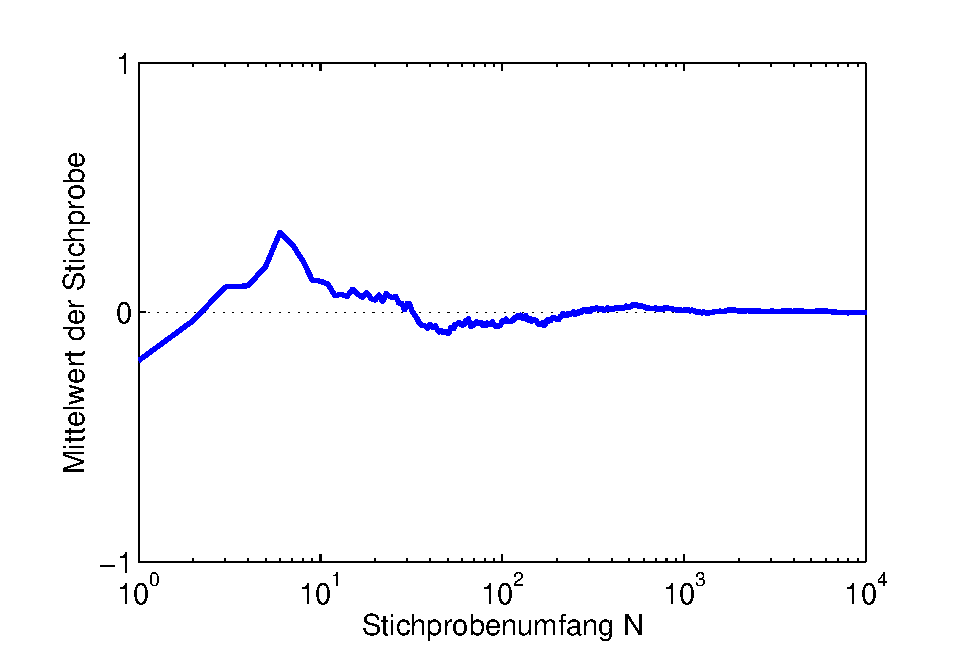
\includegraphics[width=0.5\textwidth]{Kapitel5/Bilder/image4}}
  \caption{Mittelwert einer Stichproben von einem Zufallsprozess mit $\mu$ = 0 und $\sigma$ = 0.5 als Funktion des Stichprobenumfangs N}
  \label{fig:StichprobeMittelwertStandardabweichungStichprobenumfang1}
\end{figure}

\noindent Je gr\"{o}{\ss}er der Stichprobenumfang ist, desto sicherer und genauer ist die Sch\"{a}tzung des Mittelwertes. Da die Sch\"{a}tzung erwartungstreu ist, stimmen der Mittelwert der Grundgesamtheit $\mu$ = 0 und der Mittelwert der Stichprobe $\overline{\mathrm{x}}$ f\"{u}r gro{\ss}e Stichprobenumf\"{a}nge \"{u}berein.

\subsubsection{Sch\"{a}tzen der Varianz einer Grundgesamtheit}

\noindent In Abschnitt 5.2.1 wird der Mittelwert einer Grundgesamtheit auf Basis einer Stichprobe gesch\"{a}tzt. Dabei werden die Stichprobenwerte als Zufallsvariablen x$_{1}$, ..., x$_{N}$ aufgefasst, die den Mittelwert $\mu$ und die Varianz $\sigma^{2}$ aufweisen. Im Folgenden wird die Varianz der Stichprobe betrachtet. 

\noindent Die Varianz einer Stichprobe x$_{1}$, x$_{2}$, ..., x$_{N}$ wird als Sch\"{a}tzwert der Varianz $\sigma^{2}$ der Grundgesamtheit angesehen. Die Sch\"{a}tzung ergibt

\begin{equation}\label{eq:fiveleven}
\sigma ^{2} \approx s^{2} =\dfrac{1}{N-1} \cdot \sum _{n=1}^{N}\left(x_{n} -\bar{x}\right)^{2}  =\dfrac{1}{N-1} \cdot \sum _{n=1}^{N}\left(x_{n}^{2} -\bar{x}^{2} \right)
\end{equation}

\noindent Wieder wird die Erwartungstreue der Sch\"{a}tzung untersucht. Der Erwartungswert der Stichprobenvarianz kann dargestellt werden als

\begin{equation}\label{eq:fivetwelve}
E\left(s^{2} \right)=\dfrac{1}{N-1} \cdot \left(E\left(\sum _{n=1}^{N}x_{n}^{2}  \right)-N\cdot E\left(\bar{x}^{2} \right)\right)=\dfrac{N}{N-1} \cdot \left(E\left(x^{2} \right)-E\left(\bar{x}^{2} \right)\right)
\end{equation}

\noindent Auch die Varianz $\sigma^{2}$ der Grundgesamtheit kann \"{u}ber den Erwartungswert ausgedr\"{u}ckt werden

\begin{equation}\label{eq:fivethirteen}
\sigma^{2}=E\left((x-\nu)^{2} \right) = E\left (x^{2}-\nu^{2}\right) = E\left (x^{2}\right) - \nu^{2}
\end{equation}

\noindent Auflösen nach E$\left (x^{2} \right)$ führt zu

\begin{equation}\label{eq:fivefourteen}
E\left (x^{2}\right) = \sigma_{x}^{2} + E^{2}(x) = \sigma^{2} + \nu^{2}
\end{equation}

\noindent Analog ergibt sich für die Varianz des Stichprobenmittelwertes

\begin{equation}\label{eq:fivefifteen}
E\left(\bar{x}^{2} \right)=\sigma _{\bar{x}}^{2} +E^{2} \left(\bar{x}\right)
\end{equation}

\noindent Die Varianz des Stichproben-Mittelwertes wird in Abschnitt 5.2.1 bestimmt zu $\sigma^{2}$/N, der Erwartungswert des Stichprobenwerten-Mittelwertes ist $\mu$. Durch Einsetzen folgt

\begin{equation}\label{eq:fivesixteen}
E\left(\bar{x}^{2} \right)=\sigma _{\bar{x}}^{2} +E^{2} \left(\bar{x}\right)=\dfrac{\sigma ^{2} }{N} +\mu ^{2}
\end{equation}

\noindent Mit diesen Nebenrechnungen vereinfacht sich der Erwartungswert der Stichprobenvarianz aus Gleichung \eqref{eq:fivetwelve} zu

\begin{equation}\label{eq:fiveseventeen}
E\left(s^{2} \right)=\dfrac{N}{N-1} \cdot \left(E\left(x^{2} \right)-E\left(\bar{x}^{2} \right)\right)=\dfrac{N}{N-1} \cdot \left(\sigma ^{2} +\mu ^{2} -\dfrac{\sigma ^{2} }{N} -\mu ^{2} \right)=\sigma ^{2}
\end{equation}

\noindent Der Erwartungswert der Stichprobenvarianz stimmt also mit der Varianz der Grundgesamtheit \"{u}berein. Die Sch\"{a}tzung der Varianz $\sigma^{2}$ durch die Stichprobenvarianz s$^{2}$ ist damit erwartungstreu.\newline

\noindent Zur grafischen Darstellung wird eine Stichprobe aus einem Datensatz analysiert, der eine normalverteilten Grundgesamtheit mit einem Mittelwert von $\mu$ = 0 und einer Standardabweichung von $\sigma$ = 0.5 aufweist.

\noindent 
\begin{figure}[H]
  \centerline{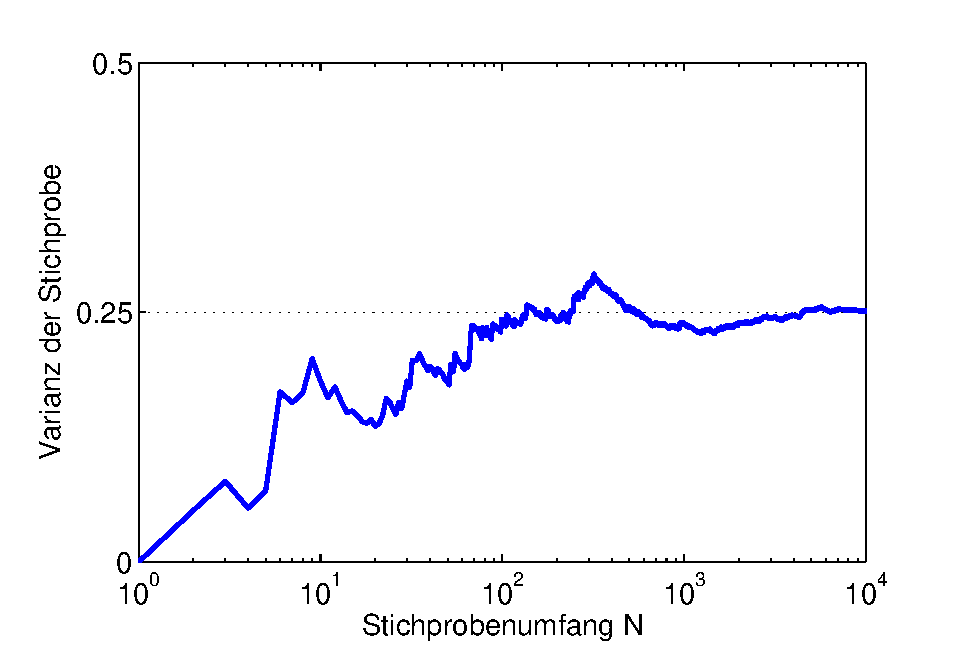
\includegraphics[width=0.5\textwidth]{Kapitel5/Bilder/image5}}
  \caption{Varianz einer Stichprobe von einem Zufallsprozess mit $\mu$ = 0 und $\sigma$ = 0.5 als Funktion des Stichprobenumfangs N}
  \label{fig:StichprobeMittelwertStandardabweichungStichprobenumfang2}
\end{figure}

\noindent Je gr\"{o}{\ss}er der Stichprobenumfang ist, desto n\"{a}her liegt die Varianz der Stichprobe an der Varianz der Grundgesamtheit $\sigma^{2}$ = 0.25.

\clearpage

\subsection{Konfidenzbereiche f\"{u}r die Sch\"{a}tzung von Parametern}

\noindent Mithilfe des arithmetischen Mittelwertes und der Varianz einer Stichprobe lassen sich die charakteristischen Parameter $\mu$ und $\sigma$ einer Normalverteilung erwartungstreu sch\"{a}tzen. Sichere Sch\"{a}tzungen von einer Stichprobe auf eine Grundgesamtheit existieren jedoch nicht. Ziel der Wahrscheinlichkeitstheorie ist deshalb, eine Wahrscheinlichkeit daf\"{u}r anzugeben, mit der zu sch\"{a}tzende Parameter in einem Intervall um ihren Sch\"{a}tzwert liegen. Zur Motivation wird dies am Beispiel eines Mittelwertes verdeutlicht.\newline

\noindent Bei der Sch\"{a}tzung des Konfidenzbereiches f\"{u}r den Mittelwert $\mu$ der Grundgesamtheit muss ein Weg gefunden werden, die Intervallgrenzen $\mu_{C1}$ und $\mu_{C2}$ zu bestimmen, die mit einer vorgegebenen Wahrscheinlichkeit $\gamma$ den wahren Mittelwert $\mu$ einschlie{\ss}en. Die Intervallgrenzen $\mu_{C1}$ und $\mu_{C2}$ m\"{u}ssen sich aus den zuf\"{a}lligen Stichprobenwerten x$_{1}$, x$_{2}$, ..., x$_{N}$ ergeben. Diese Intervallgrenzen $\mu_{C1}$ und $\mu_{C2}$ sind Funktionen von Zufallszahlen und damit selber Zufallszahlen. Wird die Wahrscheinlichkeit daf\"{u}r, dass der Mittelwert $\mu$ in dem Intervall $\mu_{C1}$ $\mathrm{<}$ $\mu$ $\leq$ $\mu_{C2}$ liegt, mit $\gamma$ bezeichnet, gilt die Gleichung

\begin{equation}\label{eq:fiveeighteen}
P\left(\mu _{C1} <\mu \le \mu _{C2} \right)=\gamma
\end{equation}

\noindent Das Intervall mit den Werten $\mu_{C1}$ und $\mu_{C2}$ als Intervallgrenzen hei{\ss}t Konfidenzintervall oder Vertrauensbereich f\"{u}r den unbekannten Parameterwert $\mu$. Die Intervallgrenzen werden auch als Konfidenzgrenzen bezeichnet. Die Wahrscheinlichkeit $\gamma$ ist die zugeh\"{o}rige Konfidenzzahl. Praktische Werte f\"{u}r $\gamma$ sind 95 \%, 99 \% oder 99.9 \%. Der Wert $\gamma$ ist die Wahrscheinlichkeit daf\"{u}r, dass ein mit einer Stichprobe bestimmtes Konfidenzintervall den wahren unbekannten Parameterwert $\mu$ enth\"{a}lt. Wird zum Beispiel eine Konfidenzzahl $\gamma$ = 95\% gew\"{a}hlt, wird davon ausgegangen, dass bei 95 \% aller Stichproben die zugeh\"{o}rigen Konfidenzintervalle den Wert $\mu$ einschlie{\ss}en. \newline 

\noindent F\"{u}r die Berechnung der Konfidenzbereiche wird von einer normalverteilten Grundgesamtheit ausgegangen. Auf Basis dieser Annahme werden die Verteilungen der beiden Stichprobenparameter f\"{u}r Mittelwert und Varianz einer normalverteilten Grundgesamtheit hergeleitet und zur Berechnung des Konfidenzintervalls verwendet. 


\subsubsection{Konfidenzbereich des Mittelwertes bei bekannter Varianz}

\noindent Mit den Zufallsvariablen x$_{1}$, ..., x$_{N}$ werden N Stichprobenwerte bezeichnet, die Teil einer Normalverteilung mit dem unbekannten Mittelwert $\mu$ und der bekannten Varianz $\sigma^{2}$ sind. Die einzelnen Stichprobenwerte sind voneinander unabh\"{a}ngig. Der Stichprobenmittelwert ergibt sich aus 

\begin{equation}\label{eq:fivenineteen}
\bar{x}=\dfrac{1}{N} \cdot \left(x_{1} +x_{2} +...+x_{N} \right)=\dfrac{1}{N} \cdot \sum _{n=1}^{N}x_{n}
\end{equation}

\noindent In Kapitel 8 wird gezeigt, dass die Summe von normalverteilten Werten selbst eine Normalverteilung besitzt. Weiterhin wird gezeigt, dass der Stichprobenmittelwert $\overline{\mathrm{x}}$ eine Normalverteilung mit dem Mittelwert

\begin{equation}\label{eq:fivetwenty}
E\left(\bar{x}\right)=\dfrac{1}{n} \cdot \left(E\left(x_{1} \right)+E\left(x_{2} \right)+...+E\left(x_{n} \right)\right)=\dfrac{n\cdot \mu }{n} =\mu 
\end{equation}

\noindent und der Varianz

\begin{equation}\label{eq:fivetwentyone}
E\left(\left(\bar{x}-\mu \right)^{2} \right)=\dfrac{\sigma ^{2} }{N}
\end{equation}

\noindent besitzt. Bei bekannter Varianz $\sigma^{2}$ der Grundgesamtheit ist auch die Varianz des Mittelwertes $\sigma^{2}$/N bekannt. Die Verteilung der Grundgesamtheit ist somit hinsichtlich aller ben\"{o}tigten Parameter spezifiziert. Auf Basis dieser Verteilung kann die Sicherheit angegeben werden, mit der der Stichprobenmittelwert $\overline{\mathrm{x}}$ in definierten Grenzen liegt. Mit der Standardisierung der Zufallsvariable

\begin{equation}\label{eq:fivetwentytwo}
z=\dfrac{\bar{x}-\mu }{\sigma _{\bar{x}} } =\dfrac{\bar{x}-\mu }{\sigma /\sqrt{N} }
\end{equation}

\noindent geht die Verteilung in eine Standardnormalverteilung \"{u}ber, sie weist also den Mittelwert $\mu_{z}$ = 0 und die Standardabweichung $\sigma_{z}$ = 1 auf. Mit dieser Verteilung wird nach Gleichung \eqref{eq:fiveeighteen} die Wahrscheinlichkeit $\gamma$, mit der die Variable z in dem Intervall c$_{1}$ ... c$_{2}$ liegt, definiert als

\begin{equation}\label{eq:fivetwentythree}
P\left(c_{1} <z\le c_{2} \right)=F\left(c_{2} \right)-F\left(c_{1} \right)=\gamma
\end{equation}

\noindent Bei Annahme eines symmetrischen Konfidenzbereiches ergeben sich die Konstanten c$_{1}$ und c$_{2}$ aus den Bedingungen

\begin{equation}\label{eq:fivetwentyfour}
F\left(c_{1} \right)=\dfrac{1-\gamma }{2}
\end{equation}

\noindent und 

\begin{equation}\label{eq:fivetwentyfive}
F\left(c_{2} \right)=1-\dfrac{1-\gamma }{2} =\dfrac{1+\gamma }{2}
\end{equation}

\noindent Dabei ist F(x) die Verteilungsfunktion der Standardnormalverteilung. Aufl\"{o}sen nach c$_{1}$ und c$_{2}$ f\"{u}hrt zu

\begin{equation}\label{eq:fivetwentysix}
c_{1} =F^{-1} \left(\dfrac{1-\gamma }{2} \right)
\end{equation}

\noindent und

\begin{equation}\label{eq:fivetwentyseven}
c_{2} =F^{-1} \left(\dfrac{1+\gamma }{2} \right)
\end{equation}

\noindent Durch Umformungen ergibt sich ein Ausdruck f\"{u}r den Konfidenzbereich des Mittelwertes der Grundgesamtheit.

\begin{equation}\label{eq:fivetwentyeight}
\gamma =P\left(c_{1} <\dfrac{\bar{x}-\mu }{\sigma /\sqrt{N} } \le c_{2} \right)=P\left(\dfrac{c_{1} \cdot \sigma }{\sqrt{N} } <\bar{x}-\mu \le \dfrac{c_{2} \cdot \sigma }{\sqrt{N} } \right)=P\left(\bar{x}-\dfrac{c_{2} \cdot \sigma }{\sqrt{N} } <\mu \le \bar{x}-\dfrac{c_{1} \cdot \sigma }{\sqrt{N} } \right)
\end{equation}

\noindent Mit der gew\"{a}hlten Wahrscheinlichkeit $\gamma$ liegt der Mittelwert $\mu$ der Grundgesamtheit in dem angegebenen Konfidenzintervall. Das Vorgehen zur Bestimmung des Konfidenzintervalls f\"{u}r den Mittelwert einer Normalverteilung mit bekannter Varianz wird in Tabelle \ref{tab:fivetwo} zusammengefasst.

\clearpage

\begin{table}[H]
\setlength{\arrayrulewidth}{.1em}
\caption{Vorgehen zur Bestimmung des Konfidenzintervalls f\"{u}r den Mittelwert einer Normalverteilung mit bekannter Varianz}
\setlength{\fboxsep}{0pt}%
\colorbox{lightgray}{%
\arrayrulecolor{white}%
\begin{tabular}{| c | c |}
\hline
\parbox[c][0.3in][c]{0.4in}{\smallskip\centering\textbf{\fontfamily{phv}\selectfont{Nr.}}} & 
\parbox[c][0.3in][c]{6.2in}{\smallskip\centering\textbf{\fontfamily{phv}\selectfont{Prozessschritt}}}\\ \hline

\parbox[c][0.3in][c]{0.4in}{\centering\fontfamily{phv}\selectfont{1}} & 
\parbox[c][0.3in][c]{6.2in}{\centering\fontfamily{phv}\selectfont{Wahl einer Konfidenzzahl $\gamma$}}\\ \hline

\parbox[c][0.9in][c]{0.4in}{\centering\fontfamily{phv}\selectfont{2}} & 
\parbox[c][0.9in][c]{6.2in}{\centering\fontfamily{phv}\selectfont{Bestimmung der zugehörigen Parameter c$_{1}$ und c$_{2}$ aus der inversen Standardnormalverteilung\\
$c_{1} =F^{-1} \left(\dfrac{1-\gamma }{2} \right) \qquad \qquad $  und $\qquad \qquad c_{2} =F^{-1} \left(\dfrac{1+\gamma }{2} \right)$}}\\ \hline

\parbox[c][0.9in][c]{0.4in}{\centering\fontfamily{phv}\selectfont{3}} & 
\parbox[c][0.9in][c]{6.2in}{\centering\fontfamily{phv}\selectfont{Berechnung des Mittelwertes aus der Stichprobe\\
$\bar{x}=\dfrac{1}{N} \cdot \left(x_{1} +x_{2} +...+x_{N} \right)=\dfrac{1}{N} \cdot \sum _{n=1}^{N}x_{n}  $}}\\ \hline

\parbox[c][0.9in][c]{0.4in}{\centering\fontfamily{phv}\selectfont{4}} & 
\parbox[c][0.9in][c]{6.2in}{\centering\fontfamily{phv}\selectfont{Bestimmung des Konfidenzintervalls\\
$\bar{x}-\dfrac{c_{2} \cdot \sigma }{\sqrt{N} } <\mu \le \bar{x}-\dfrac{c_{1} \cdot \sigma }{\sqrt{N} } $}}\\ \hline

\end{tabular}%
}
\label{tab:fivetwo}
\end{table}

\noindent Die Zusammenh\"{a}nge zwischen Stichprobenumfang, Konfidenzintervall und Aussagesicherheit sollen in den folgenden Abbildungen interpretiert werden. Die L\"{a}nge L eines Konfidenzintervalls ist nach Gleichung \eqref{eq:fivetwentyeight}

\begin{equation}\label{eq:fivetwentynine}
L=\dfrac{\left(c_{2} -c_{1} \right)\cdot \sigma}{\sqrt{N}}
\end{equation}

\noindent Zur Verkleinerung des Konfidenzintervalls muss der Stichprobenumfang vergr\"{o}{\ss}ert werden, oder es m\"{u}ssen Kompromisse hinsichtlich der Aussagesicherheit eingegangen werden. Bild \ref{fig:Konfidenzintervall1} stellt f\"{u}r unterschiedliche Konfidenzzahlen $\gamma$ die L\"{a}nge des Konfidenzintervalls als Funktion des Stichprobenumfangs N dar. 

\noindent 
\begin{figure}[H]
  \centerline{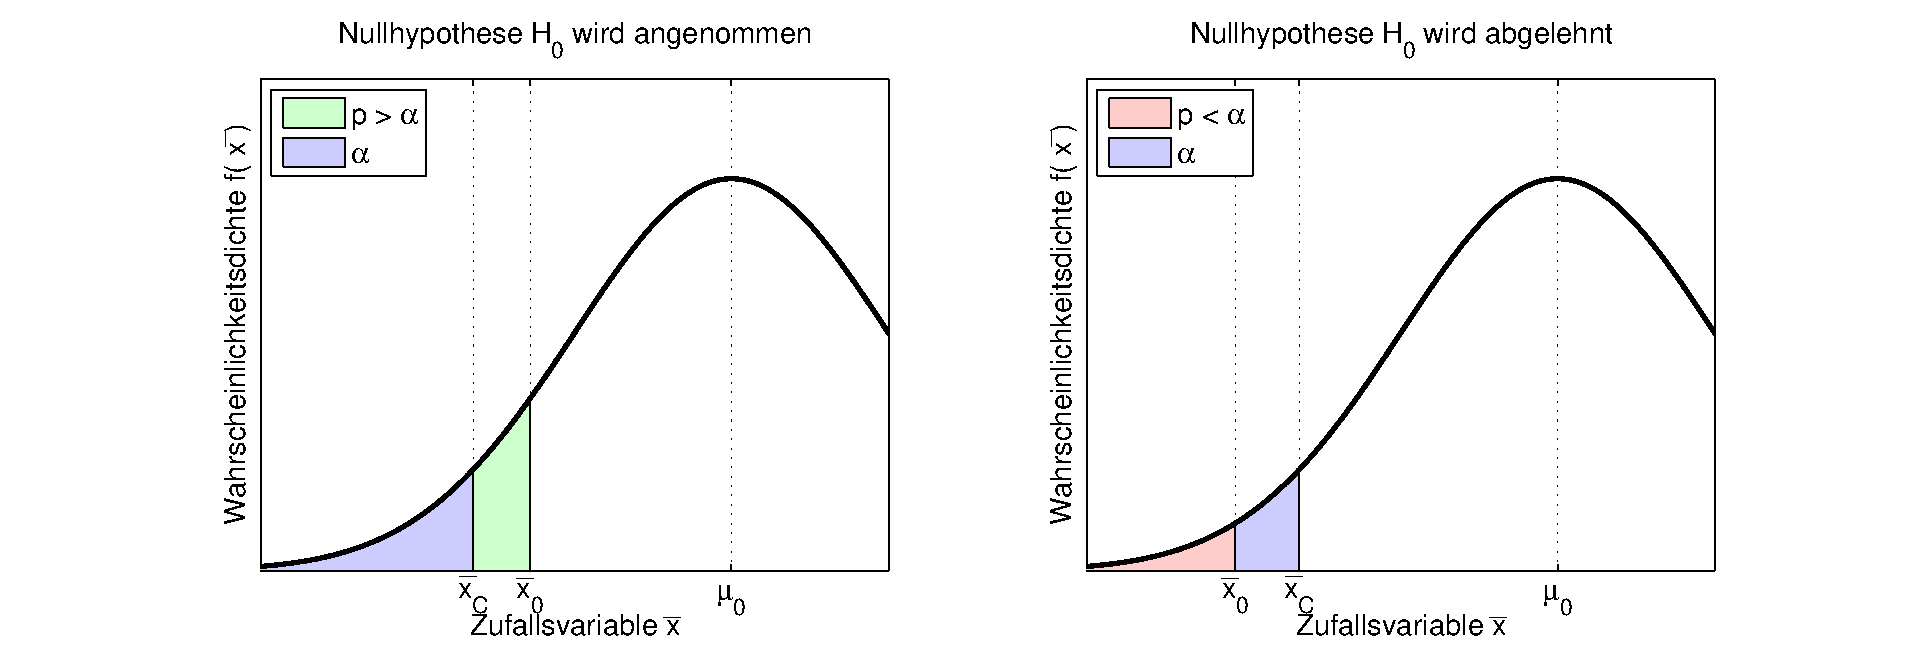
\includegraphics[width=0.5\textwidth]{Kapitel5/Bilder/image6}}
  \caption{L\"{a}nge des Konfidenzintervalls als Funktion des Stichprobenumfangs N}
  \label{fig:Konfidenzintervall1}
\end{figure}

\noindent Durch Aufl\"{o}sen von Gleichung \eqref{eq:fivetwentynine} nach N kann die Anzahl von Stichproben bestimmt werden, die notwendig ist, den Mittelwert mit einem Konfidenzintervall der L\"{a}nge L und der Wahrscheinlichkeit $\gamma$ zu bestimmen. 

\begin{equation}\label{eq:fivethirty}
N=\dfrac{\left(c_{2} -c_{1} \right)^{2} \cdot \sigma ^{2}}{L^{2}}
\end{equation}

\noindent Bild \ref{fig:Konfidenzintervall2} stellt f\"{u}r unterschiedliche Verh\"{a}ltnisse von L\"{a}nge des Konfidenzbereiches L und Standardabweichung der Grundgesamtheit $\sigma$ den Stichprobenumfang N als Funktion der Konfidenzzahl $\gamma$ dar. Der Stichprobenumfang steigt mit steigendem Genauigkeitsanspruch an die Sch\"{a}tzung und mit steigender Sicherheit der Aussage. 

\noindent 
\begin{figure}[H]
  \centerline{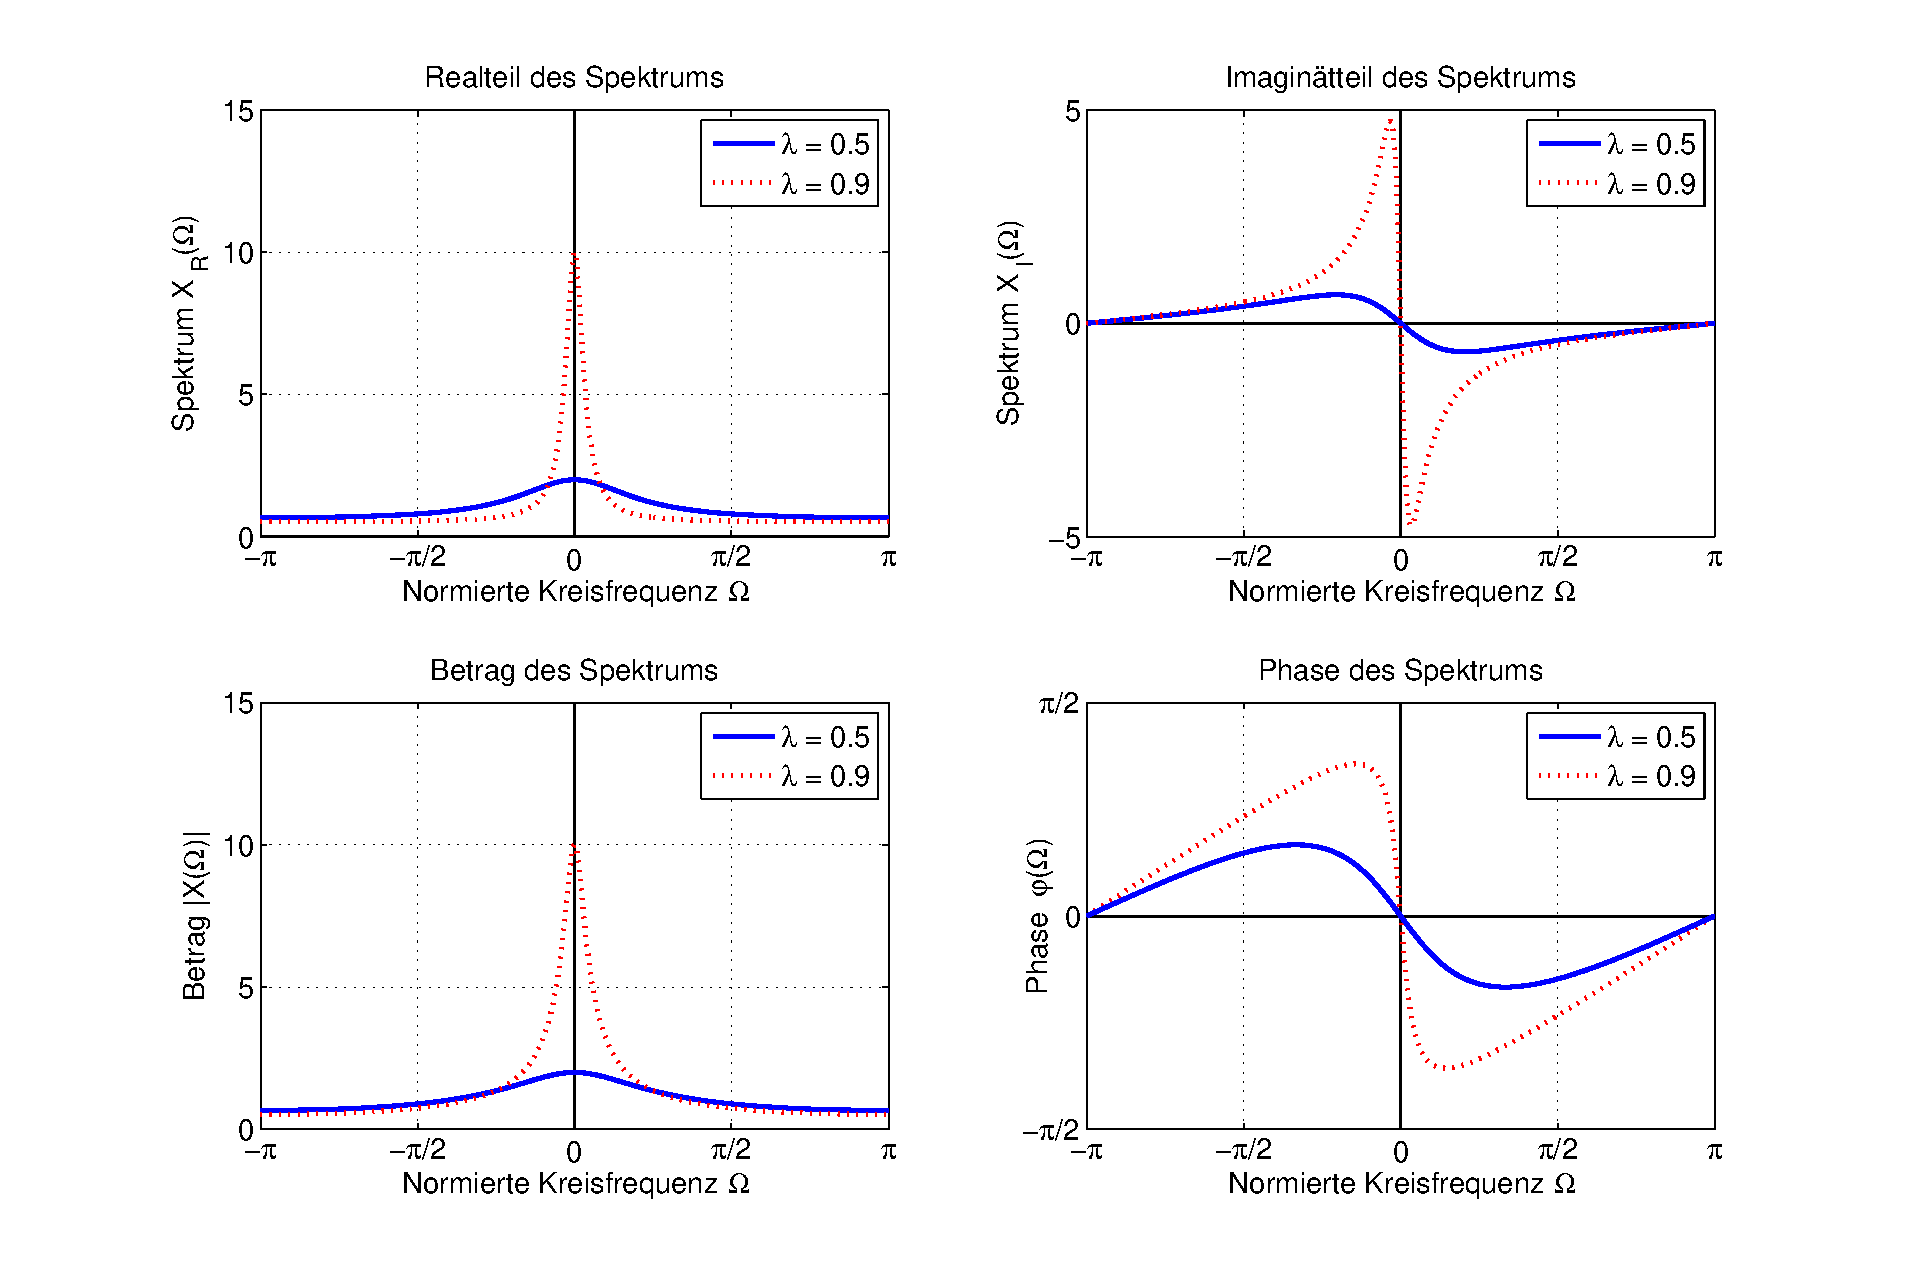
\includegraphics[width=0.5\textwidth]{Kapitel5/Bilder/image7}}
  \caption{Stichprobenumfang n als Funktion der Konfidenzzahl $\gamma$}
  \label{fig:Konfidenzintervall2}
\end{figure}

\noindent
\colorbox{lightgray}{%
\arrayrulecolor{white}%
\renewcommand\arraystretch{0.6}%
\begin{tabular}{ wl{16.5cm} }
{\fontfamily{phv}\selectfont
\noindent{Beispiel: 5 V Linearregler}}
\end{tabular}%
}\bigskip

\noindent Bei der Vermessung von 5 V Linearreglern wird eine Stichprobe von N = 100 Teilen analysiert. Es soll das 95\% Konfidenzintervall f\"{u}r den Mittelwert der entsprechenden Normalverteilung mit der bekannten Varianz $\sigma^{2}$ = 0.09 werden.

\noindent Der Mittelwert der Stichprobe betr\"{a}gt 5.000 V. Es wird die Konfidenzzahl $\gamma$ = 0.95 gefordert, zu der die kritischen Parameter c$_{1}$ = - 1.96 und c$_{2}$ = 1.96 geh\"{o}ren. Mit dem berechneten Mittelwert ergeben sich die Grenzen des Konfidenzintervalls zu

\begin{equation}\label{eq:fivethirtyone}
\mu \ge \bar{x}-\dfrac{c_{2} \cdot \sigma}{\sqrt{N}} =5-\dfrac{1.96\cdot 0.3}{10} = 4.9412
\end{equation}

\noindent und

\begin{equation}\label{eq:fivethirtytwo}
\mu \le \bar{x}-\dfrac{c_{1} \cdot \sigma}{\sqrt{N}} =5-\dfrac{-1.96\cdot 0.3}{10} = 5.0588
\end{equation}

\noindent F\"{u}r das Beispiel soll jetzt der notwendige Stichprobenumfang N f\"{u}r ein 95\%-Konfidenzintervall mit der L\"{a}nge L = 0.01 bestimmt werden. Nach Gleichung \eqref{eq:fivethirty} ergibt sich f\"{u}r den vorliegenden Fall

\begin{equation}\label{eq:fivethirtythree}
N=\dfrac{\left(c_{2} -c_{1} \right)^{2} \cdot \sigma ^{2} }{L^{2} } =\dfrac{\left(1.96+1.96\right)^{2} \cdot 0.09}{0.0001} = 13830
\end{equation}

\clearpage

\subsubsection{Konfidenzbereich der Varianz}

\noindent Ist die Varianz der Grundgesamtheit nicht bekannt, muss die Varianz der Grundgesamtheit mithilfe der Stichprobe gesch\"{a}tzt werden. Allgemein gilt f\"{u}r die Varianz einer Stichprobe 

\begin{equation}\label{eq:fivethirtyfour}
s_{x}^{2} =\dfrac{1}{N-1} \cdot \sum _{n=1}^{N}\left(x_{n} -\bar{x}\right)^{2}
\end{equation}

\noindent Damit die in Kapitel 4 eingef\"{u}hrten Pr\"{u}f- und Testverteilungen verwendet werden k\"{o}nnen, wird die Variable x standardisiert. Dazu wird die Variable z eingef\"{u}hrt. 

\begin{equation}\label{eq:fivethirtyfive}
z_{n} =\dfrac{x_{n} -\mu }{\sigma }
\end{equation}

\noindent Sie besitzt den Mittelwert

\begin{equation}\label{eq:fivethirtysix}
\bar{z}=\dfrac{1}{N} \cdot \sum _{n=1}^{N}\dfrac{x_{n} -\mu }{\sigma}  =\dfrac{\bar{x}-\mu }{\sigma}
\end{equation}

\noindent F\"{u}r die Standardabweichungen der Zufallsvariable z ergibt sich 

\begin{equation}\label{eq:fivethirtyseven}
s_{z}^{2} =\dfrac{1}{N-1} \cdot \sum _{n=1}^{N}\left(z_{n} -\bar{z}\right)^{2}  =\dfrac{1}{N-1} \cdot \sum _{n=1}^{N}\left(\dfrac{x_{n} -\mu }{\sigma } -\dfrac{\bar{x}-\mu }{\sigma } \right)^{2}  =\dfrac{1}{N-1} \cdot \sum _{n=1}^{N}\left(\dfrac{x_{n} -\bar{x}}{\sigma } \right)^{2}
\end{equation}

Bei dem Ausdruck f\"{u}r s$_{Z2}$ handelt es sich um die Quadratsumme einer standardnormalverteilten Gr\"{o}{\ss}e. Nach den Ausf\"{u}hrungen zur Chi-Quadrat-Verteilung und Gleichung \eqref{eq:fivethirtyseven} ist damit die Gr\"{o}{\ss}e

\begin{equation}\label{eq:fivethirtyeight}
\chi =\left(N-1\right)\cdot s_{z}^{2} =\sum _{n=1}^{N}\left(\dfrac{x_{n} -\bar{x}}{\sigma } \right)^{2}
\end{equation}

chi-quadrat-verteilt mit N - 1 Freiheitsgraden. Um die Varianz der Stichprobe s$_{x2}$ und die Varianz der Grundgesamtheit $\sigma^{2}$ in Verbindung zu bringen, wird Gleichung \eqref{eq:fivethirtyeight} umgeformt zu

\begin{equation}\label{eq:fivethirtynine}
\chi =\sum _{n=1}^{N}\left(\dfrac{x_{n} -\bar{x}}{\sigma } \right)^{2}  =\dfrac{N-1}{\sigma ^{2} } \cdot \dfrac{1}{N-1} \cdot \sum _{n=1}^{N}\left(x_{n} -\bar{x}\right)^{2}  =\dfrac{N-1}{\sigma ^{2} } \cdot s_{x}^{2} =\dfrac{s_{x}^{2} }{\sigma ^{2} } \cdot (N-1)
\end{equation}

\noindent Das Verh\"{a}ltnis der beiden Varianzen kann demnach \"{u}ber die Chi-Quadrat-Verteilung beschrieben werden. Zur Herleitung des Konfidenzintervalls f\"{u}r $\sigma^{2}$ wird \"{u}ber die Wahrscheinlichkeit daf\"{u}r berechnet, dass die Variable  in einem Intervall c$_{1}$ $\mathrm{<}$ $\chi$ $\leq$ c$_{2}$ liegt.

\begin{equation}\label{eq:fivefourty}
P\left(c_{1} \le \chi \le c_{2} \right)=\gamma
\end{equation}

Bei Annahme eines symmetrischen Konfidenzbereiches ergeben sich die Konstanten c$_{1}$ und c$_{2}$ aus den Bedingungen

\begin{equation}\label{eq:fivefourtyone}
F\left(c_{1} \right)=\dfrac{1-\gamma }{2}
\end{equation}

\noindent und 

\begin{equation}\label{eq:fivefourtytwo}
F\left(c_{2} \right)=1-\dfrac{1-\gamma }{2} =\dfrac{1+\gamma }{2}
\end{equation}

\noindent Dabei ist F(x) die Verteilungsfunktion der Chi-Quadrat-Verteilung mit N - 1 Freiheitsgraden. Aufl\"{o}sen nach c$_{1}$ und c$_{2}$ f\"{u}hrt zu

\begin{equation}\label{eq:fivefourtythree}
c_{1} =F^{-1} \left(\dfrac{1-\gamma }{2} \right)
\end{equation}

\noindent und

\begin{equation}\label{eq:fivefourtyfour}
c_{2} =F^{-1} \left(\dfrac{1+\gamma }{2} \right)
\end{equation}

\noindent Durch Umformungen ergibt sich der Konfidenzbereich f\"{u}r die Varianz der Grundgesamtheit.

\begin{equation}\label{eq:fivefourtyfive}
\gamma =P\left(c_{1} <\dfrac{s^{2} }{\sigma ^{2}} \cdot (N-1)\le c_{2} \right)=P\left(\dfrac{1}{c_{1}} \ge \dfrac{\sigma ^{2}}{s^{2} \cdot (N-1)} >\dfrac{1}{c_{2}} \right)=P\left(\dfrac{s^{2} \cdot (N-1)}{c_{2}} <\sigma ^{2} \le \dfrac{s^{2} \cdot (N-1)}{c_{1}} \right)
\end{equation}

\noindent Mit der gew\"{a}hlten Wahrscheinlichkeit $\gamma$ liegt die Varianz $\sigma^{2}$ der Grundgesamtheit in dem angegebenen Konfidenzintervall. Das Vorgehen zur Bestimmung des Konfidenzintervalls f\"{u}r die Varianz einer Normalverteilung wird in Tabelle \ref{tab:fivethree} zusammengefasst.

\begin{table}[H]
\setlength{\arrayrulewidth}{.1em}
\caption{Vorgehen zur Bestimmung des Konfidenzintervalls f\"{u}r die Varianz einer Normalverteilung}
\setlength{\fboxsep}{0pt}%
\colorbox{lightgray}{%
\arrayrulecolor{white}%
\begin{tabular}{| c | c |}
\hline
\parbox[c][0.3in][c]{0.4in}{\smallskip\centering\textbf{\fontfamily{phv}\selectfont{Nr.}}} & 
\parbox[c][0.3in][c]{6.2in}{\smallskip\centering\textbf{\fontfamily{phv}\selectfont{Prozessschritt}}}\\ \hline

\parbox[c][0.3in][c]{0.4in}{\centering\fontfamily{phv}\selectfont{1}} & 
\parbox[c][0.3in][c]{6.2in}{\centering\fontfamily{phv}\selectfont{Wahl einer Konfidenzzahl $\gamma$}}\\ \hline

\parbox[c][0.9in][c]{0.4in}{\centering\fontfamily{phv}\selectfont{2}} & 
\parbox[c][0.9in][c]{6.2in}{\centering\fontfamily{phv}\selectfont{Bestimmung der zugeh\"{o}rigen Parameter c${}_{1}$ und c${}_{2}$ aus der inversen Chi-Quadrat-Verteilung mit N - 1 Freiheitsgraden \\  
$c_{1} =F^{-1} \left(\dfrac{1-\gamma }{2} \right)\qquad\qquad $  und  $\qquad\qquad c_{2} =F^{-1} \left(\dfrac{1+\gamma }{2} \right)$}}\\ \hline

\parbox[c][0.9in][c]{0.4in}{\centering\fontfamily{phv}\selectfont{3}} & 
\parbox[c][0.9in][c]{6.2in}{\centering\fontfamily{phv}\selectfont{Berechnung der Varianz aus der Stichprobe\\
$s^{2} =\dfrac{1}{N-1} \cdot \sum _{n=1}^{N}\left(x_{n} -\bar{x}\right)^{2}  $}}\\ \hline

\parbox[c][0.9in][c]{0.4in}{\centering\fontfamily{phv}\selectfont{4}} & 
\parbox[c][0.9in][c]{6.2in}{\centering\fontfamily{phv}\selectfont{Bestimmung des Konfidenzintervalls\\
$\dfrac{s^{2} \cdot \left(N-1\right)}{c_{2} } <\sigma ^{2} \le \dfrac{s^{2} \cdot \left(N-1\right)}{c_{1} } $}}\\ \hline

\end{tabular}%
}
\label{tab:fivethree}
\end{table}

\noindent
\colorbox{lightgray}{%
\arrayrulecolor{white}%
\renewcommand\arraystretch{0.6}%
\begin{tabular}{ wl{16.5cm} }
{\fontfamily{phv}\selectfont
\noindent{Beispiel: Gewicht von Klebermengen}}
\end{tabular}%
}\bigskip

\noindent In einem Beispiel werden die Varianz f\"{u}r das Gewicht von Klebermengen eines Fertigungsprozesses und ihr Konfidenzbereich bestimmt. Es soll das 95\%-Konfidenzintervall f\"{u}r die Varianz $\sigma^{2}$ der Grundgesamtheit f\"{u}r die folgende Stichprobe berechnet werden. Dabei wird vorausgesetzt, dass die Grundgesamtheit normalverteilt ist.

\begin{table}[H]
\setlength{\arrayrulewidth}{.1em}
\caption{Stichprobe f\"{u}r das Gewicht von Klebemengen in einem Fertigungsprozess}
\setlength{\fboxsep}{0pt}%
\colorbox{lightgray}{%
\arrayrulecolor{white}%
\begin{tabular}{| wc{2.4cm} | wc{1cm} | wc{1cm} | wc{1cm} | wc{1cm} | wc{1cm} | wc{1cm} | wc{1cm} | wc{1cm} | wc{1cm} | wc{1cm} }
\hline\xrowht{15pt}

\fontfamily{phv}\selectfont\textbf{Stichprobe} & 1 & 2 & 3 & 4 & 5 & 6 & 7 & 8 & 9 & 10 \\ \hline \xrowht{25pt}

\fontfamily{phv}\selectfont\textbf{Gewicht x / g} & 4.3 & 4.5 & 4.2 & 4.3 & 4.3 & 4.7 & 4.4 & 4.2 & 4.3 & 4.5\\ \hline

\end{tabular}%
}
\label{tab:fivefour}
\end{table}

\noindent Es ist eine Konfidenzzahl von $\gamma$ = 0.95 gefordert. Wegen N = 10 ergeben sich aus der inversen Chi-Quadrat-Verteilung mit 10 - 1 = 9 Freiheitsgraden c$_{1}$ = 2.7 und c$_{2}$ = 19.02. Die Auswertung der Stichprobe ergibt eine Varianz von

\begin{equation}\label{eq:fivefourtysix}
s^{2} =\dfrac{1}{N-1} \cdot \sum _{n=1}^{N}\left(x_{n} -\bar{x}\right)^{2}  = 0.0246 g^{2} 
\end{equation}

\noindent Damit lautet das Konfidenzintervall

\begin{equation}\label{eq:fivefourtyseven}
0.0116 g^{2} <\sigma ^{2} \le  0.0818 g^{2}
\end{equation}

\subsubsection{Konfidenzbereich des Mittelwertes bei unbekannter Varianz}

\noindent Ist die Varianz der Grundgesamtheit nicht bekannt, kann die in Abschnitt 5.3.1 hergeleitete Standardnormalverteilung nicht verwendet werden. Zur Herleitung der zugrunde liegenden Verteilung wird zun\"{a}chst wieder die Gr\"{o}{\ss}e

\begin{equation}\label{eq:fivefourtyeight}
z=\dfrac{\bar{x}-\mu }{\sigma /\sqrt{N}}
\end{equation}

\noindent betrachtet. Sie weist nach den Ausf\"{u}hrungen in Abschnitt 5.3.1 eine Standardnormalverteilung auf. Die Herleitung in Gleichung \eqref{eq:fivefourtynine} zeigt, dass die Gr\"{o}{\ss}e 

\begin{equation}\label{eq:fivefourtynine}
\dfrac{\chi }{N-1} =\dfrac{s^{2} }{\sigma ^{2}}
\end{equation}

\noindent eine Chi-Quadrat-Verteilung mit N - 1 Freiheitsgraden besitzt. Nach den Ausf\"{u}hrungen zu Testverteilungen besitzt die Zufallsvariable

\begin{equation}\label{eq:fivefifty}
t=\dfrac{\dfrac{\bar{x}-\mu}{\sigma /\sqrt{N}}}{\sqrt{\dfrac{s^{2}}{\sigma ^{2}} } } =\dfrac{\bar{x}-\mu}{s/\sqrt{N}}
\end{equation}

\noindent damit eine t-Verteilung mit N - 1 Freiheitsgraden. Damit ist auch bei unbekannter Varianz der Grundgesamtheit die Verteilung f\"{u}r den Stichprobenmittelwert $\overline{\mathrm{x}}$ bestimmt, und es kann die Sicherheit angegeben werden, mit der der Stichprobenmittelwert $\overline{\mathrm{x}}$ in definierten Grenzen liegt. Dazu wird eine Konfidenzzahl $\gamma$ festgelegt, f\"{u}r die gilt

\begin{equation}\label{eq:fivefiftyone}
P\left(c_{1} <t\le c_{2} \right)=F\left(c_{2} \right)-F\left(c_{1} \right)=\gamma
\end{equation}

\noindent Bei Annahme eines symmetrischen Konfidenzbereiches ergeben sich die Konstanten c$_{1}$ und c$_{2}$ aus den Bedingungen

\begin{equation}\label{eq:fivefiftytwo}
F\left(c_{1} \right)=\dfrac{1-\gamma}{2}
\end{equation}

\noindent und 

\begin{equation}\label{eq:fivefiftythree}
F\left(c_{2} \right)=1-\dfrac{1-\gamma}{2} =\dfrac{1+\gamma}{2}
\end{equation}

\noindent Dabei ist F(x) die Verteilungsfunktion der t-Verteilung mit N - 1 Freiheitsgraden. Aufl\"{o}sen nach c$_{1}$ und c$_{2}$ f\"{u}hrt zu

\begin{equation}\label{eq:fivefiftyfour}
c_{1} =F^{-1} \left(\dfrac{1-\gamma }{2} \right)
\end{equation}

\noindent und

\begin{equation}\label{eq:fivefiftyfive}
c_{2} =F^{-1} \left(\dfrac{1+\gamma }{2} \right)
\end{equation}

\noindent Durch Umformungen ergibt sich ein Ausdruck f\"{u}r den Konfidenzbereich des Mittelwertes der Grundgesamtheit bei unbekannter Varianz.

\begin{equation}\label{eq:fivefiftysix}
\gamma =P\left(c_{1} <\sqrt{N} \cdot \dfrac{\bar{x}-\mu }{s} \le c_{2} \right)=P\left(\dfrac{c_{1} \cdot s}{\sqrt{N} } <\bar{x}-\mu \le \dfrac{c_{2} \cdot s}{\sqrt{N} } \right)=P\left(\bar{x}-\dfrac{c_{2} \cdot s}{\sqrt{N} } <\mu \le \bar{x}-\dfrac{c_{1} \cdot s}{\sqrt{N} } \right)
\end{equation}

\noindent Mit der gew\"{a}hlten Wahrscheinlichkeit $\gamma$ liegt der Mittelwert $\mu$ der Grundgesamtheit in dem angegebenen Konfidenzintervall. Das Vorgehen zur Bestimmung des Konfidenzintervalls f\"{u}r den Mittelwert einer Normalverteilung mit unbekannter Varianz wird in Tabelle \ref{tab:fivefive} zusammengefasst.

\begin{table}[H]
\setlength{\arrayrulewidth}{.1em}
\caption{Vorgehen zur Bestimmung des Konfidenzintervalls f\"{u}r den Mittelwert einer Normalverteilung mit unbekannter Varianz}
\setlength{\fboxsep}{0pt}%
\colorbox{lightgray}{%
\arrayrulecolor{white}%
\begin{tabular}{| c | c |}
\hline
\parbox[c][0.3in][c]{0.4in}{\smallskip\centering\textbf{\fontfamily{phv}\selectfont{Nr.}}} & 
\parbox[c][0.3in][c]{6.2in}{\smallskip\centering\textbf{\fontfamily{phv}\selectfont{Prozessschritt}}}\\ \hline

\parbox[c][0.3in][c]{0.4in}{\centering\fontfamily{phv}\selectfont{1}} & 
\parbox[c][0.3in][c]{6.2in}{\centering\fontfamily{phv}\selectfont{Wahl einer Konfidenzzahl $\gamma$}}\\ \hline

\parbox[c][0.9in][c]{0.4in}{\centering\fontfamily{phv}\selectfont{2}} & 
\parbox[c][0.9in][c]{6.2in}{\centering\fontfamily{phv}\selectfont{Bestimmung der zugeh\"{o}rigen Parameter c${}_{1}$ und c${}_{2}$ aus der inversen Chi-Quadrat-Verteilung mit N - 1 Freiheitsgraden \\  
$c_{1} =F^{-1} \left(\dfrac{1-\gamma }{2} \right)\qquad\qquad $  und  $\qquad\qquad c_{2} =F^{-1} \left(\dfrac{1+\gamma }{2} \right)$}}\\ \hline

\parbox[c][0.9in][c]{0.4in}{\centering\fontfamily{phv}\selectfont{3}} & 
\parbox[c][0.9in][c]{6.2in}{\centering\fontfamily{phv}\selectfont{Berechnung der Varianz aus der Stichprobe\\
$\bar{x}=\dfrac{1}{N} \cdot \sum _{n=1}^{N}x_{n} \qquad\qquad $ und  $\qquad\qquad s=\sqrt{\dfrac{1}{N-1} \cdot \sum _{n=1}^{N}\left(x_{n} -\bar{x}\right)^{2}}$ }}\\ \hline

\parbox[c][0.9in][c]{0.4in}{\centering\fontfamily{phv}\selectfont{4}} & 
\parbox[c][0.9in][c]{6.2in}{\centering\fontfamily{phv}\selectfont{Bestimmung des Konfidenzintervalls\\
$\bar{x}-\dfrac{c_{2} \cdot s}{\sqrt{N} } <\mu \le \bar{x}-\dfrac{c_{1} \cdot s}{\sqrt{N} } $}}\\ \hline

\end{tabular}%
}
\label{tab:fivefive}
\end{table}

\noindent Um den Unterschied zwischen den beiden F\"{a}llen einer bekannten Varianz und einer unbekannten Varianz zu diskutieren, zeigt Bild \ref{fig:Konfidenzintervall3} das Verh\"{a}ltnis der L\"{a}nge L$_{T}$ des Konfidenzintervalls bei unbekannter Varianz und der L\"{a}nge L$_{Z}$ des Konfidenzintervalls bei bekannter Varianz als Funktion des Stichprobenumfangs N.

\noindent 
\begin{figure}[H]
  \centerline{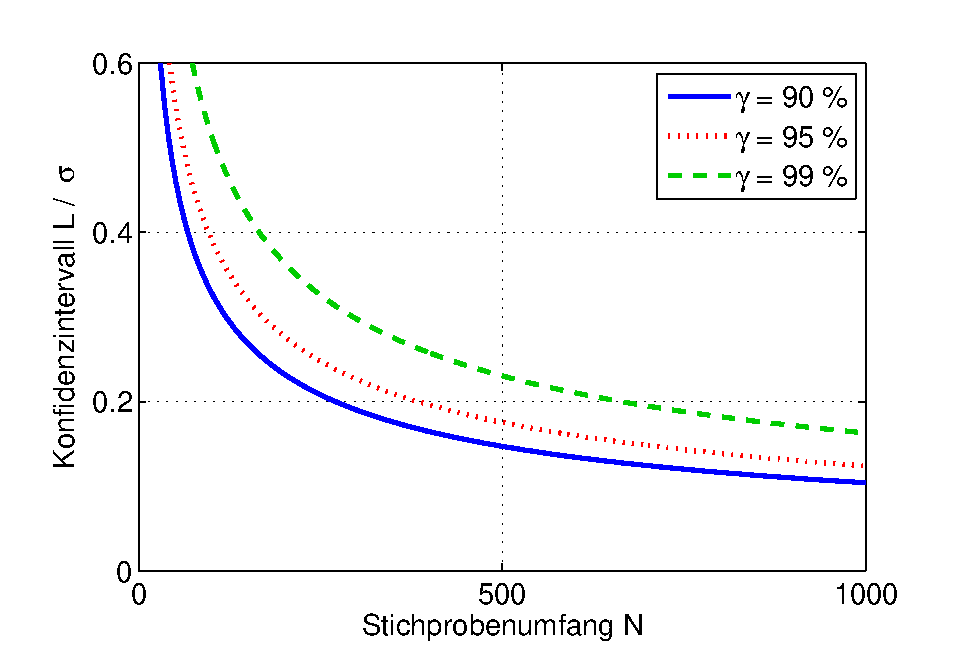
\includegraphics[width=0.5\textwidth]{Kapitel5/Bilder/image8}}
  \caption{Verh\"{a}ltnis der L\"{a}nge L${}_{T}$ des Konfidenzintervalls bei unbekannter Varianz und der L\"{a}nge L${}_{Z}$ des Konfidenzintervalls bei bekannter Varianz als Funktion des Stichprobenumfangs N}
  \label{fig:Konfidenzintervall3}
\end{figure}

\noindent Bei einer hinreichend gro{\ss}en Stichprobe unterscheiden sich die L\"{a}ngen der beiden Konfidenzintervalle nur wenig. Je kleiner der Stichprobenumfang N wird, desto gr\"{o}{\ss}er ist der Unterschied. Zus\"{a}tzlich steigt der Unterschied mit steigender Konfidenzzahl $\gamma$ an. \bigskip

\noindent
\colorbox{lightgray}{%
\arrayrulecolor{white}%
\renewcommand\arraystretch{0.6}%
\begin{tabular}{ wl{16.5cm} }
{\fontfamily{phv}\selectfont
\noindent{Beispiel: Gewicht von Klebermengen}}
\end{tabular}%
}\medskip

\noindent In einem Beispiel wird der Mittelwert und Konvergenzbereich f\"{u}r das Gewicht von Klebermengen eines Fertigungsprozesses bestimmt. Die Daten sind in Tabelle \ref{tab:fivefive} aufgef\"{u}hrt. Es soll das 95\%-Konfidenzintervall f\"{u}r den Mittelwert µ der Grundgesamtheit berechnet werden. Dabei wird vorausgesetzt, dass die Grundgesamtheit normalverteilt ist.

\noindent Es ist eine Konfidenzzahl von $\gamma$ = 0.95 gefordert. Mit N = 10 Stichproben ergeben sich die Parameter c$_{1}$ = - 2.2622 und c$_{2}$ = 2.2622. Die Auswertung der Stichprobe ergibt f\"{u}r den arithmetischen Mittelwert

\begin{equation}\label{eq:fivefiftyseven}
\bar{x}=\dfrac{1}{N} \cdot \sum _{n=1}^{N}x_{n}  =4.37 g
\end{equation}

\noindent und f\"{u}r die Standardabweichung

\begin{equation}\label{eq:fivefiftyeight}
s=\sqrt{\dfrac{1}{N-1} \cdot \sum _{n=1}^{N}\left(x_{n} -\bar{x}\right)^{2}} =0.157 g
\end{equation}

\noindent Mit diesen Werten ergibt sich das Konfidenzintervall zu

\begin{equation}\label{eq:fivefiftynine}
KONF\left(4.258 g\le \mu \le 4.482 g\right)
\end{equation}

\clearpage

\subsubsection{Zusammenfassung der Konfidenzbereiche f\"{u}r die Sch\"{a}tzung von Parametern}

\noindent Die Sch\"{a}tzung des Konfidenzbereiches beruht in allen F\"{a}llen auf einer Zufallsvariable mit einer bekannten Verteilung, in deren Beschreibung der gesuchte Parameter der Grundgesamtheit und der bekannte Parameter der Stichprobe vorkommen. F\"{u}r die bekannte Zufallsvariable wird der Konfidenzbereich f\"{u}r ein Signifikanzniveau $\gamma$ bestimmt. Durch Umformen dieser Gleichung ergibt sich der Konfidenzbereich der gesuchten Gr\"{o}{\ss}e.\newline

\noindent Zur Absch\"{a}tzung der Aussagesicherheit von Mittelwert µ und Standardabweichung $\sigma$ einer normalverteilten Grundgesamtheit ergeben sich die in Tabelle \ref{tab:fivesix} dargestellten Verteilungen und Konfidenzbereiche.

\begin{table}[H]
\setlength{\arrayrulewidth}{.1em}
\caption{Verteilungen und Konfidenzbereiche von Stichproben normalverteilter Grundgesamtheiten}
\setlength{\fboxsep}{0pt}%
\colorbox{lightgray}{%
\arrayrulecolor{white}%
\begin{tabular}{| c | c | c |}
\hline
\parbox[c][0.3in][c]{1.8in}{\smallskip\centering\textbf{\fontfamily{phv}\selectfont{ }}} & 
\parbox[c][0.3in][c]{2.25in}{\smallskip\centering\textbf{\fontfamily{phv}\selectfont{Verteilung der Schätzfunktion}}} & 
\parbox[c][0.3in][c]{2.25in}{\smallskip\centering\textbf{\fontfamily{phv}\selectfont{Konfidenzbereich}}}\\ \hline

\parbox[c][1in][c]{1.8in}{\centering\fontfamily{phv}\selectfont\textbf{Mittelwert $\mu$\\ bei bekannter Varianz}} & 
\parbox[c][1in][c]{2.25in}{\centering\fontfamily{phv}\selectfont{Standardnormalverteilung\\

$z=\dfrac{\bar{x}-\mu }{\sigma /\sqrt{N} }$}} & 
\parbox[c][1in][c]{2.25in}{\centering\fontfamily{phv}\selectfont{$\bar{x}-\dfrac{c_{2} \cdot \sigma}{\sqrt{N}} <\mu \le \bar{x}-\dfrac{c_{1} \cdot \sigma}{\sqrt{N}}$}}\\ \hline

\parbox[c][1in][c]{1.8in}{\centering\fontfamily{phv}\selectfont\textbf{Varianz $\sigma^{2}$}} & 
\parbox[c][1in][c]{2.25in}{\centering\fontfamily{phv}\selectfont{Chi-Quadrat-Verteilung mit N - 1 Freiheitsgraden\\

$z=\dfrac{\bar{x}-\mu }{\sigma /\sqrt{N} }$}} & 
\parbox[c][1in][c]{2.25in}{\centering\fontfamily{phv}\selectfont{$\bar{x}-\dfrac{c_{2} \cdot \sigma}{\sqrt{N}} <\mu \le \bar{x}-\dfrac{c_{1} \cdot \sigma}{\sqrt{N}}$}}\\ \hline

\parbox[c][1in][c]{1.8in}{\centering\fontfamily{phv}\selectfont\textbf{Mittelwert $\mu$\\ bei unbekannter Varianz }} & 
\parbox[c][1in][c]{2.25in}{\centering\fontfamily{phv}\selectfont{t-Verteilung mit N - 1 Freiheitsgraden\\

$\bar{x}-\dfrac{c_{2} \cdot s}{\sqrt{N} } <\mu \le \bar{x}-\dfrac{c_{1} \cdot s}{\sqrt{N} } $}} & 
\parbox[c][1in][c]{2.25in}{\centering\fontfamily{phv}\selectfont{$t=\dfrac{\bar{x}-\mu }{s/\sqrt{N} } $}}\\ \hline

\end{tabular}%
}
\label{tab:fivesix}
\end{table}

\clearpage

\subsection{Konfidenzbereiche f\"{u}r den Vergleich von Stichproben}

\noindent In Anschnitt 5.3 werden Konfidenzbereiche f\"{u}r Parameter von Zufallsvariablen berechnet. Bei der Auswertung von Labor-Versuchen tritt au{\ss}erdem der Fall auf, dass zwei Stichproben x$_{11}$, x$_{12}$, {\dots}, x$_{1N}$ und x$_{21}$, x$_{22}$, {\dots}, x$_{2M}$ miteinander verglichen werden sollen. In diesem Abschnitt wird gezeigt, welche Schl\"{u}sse dabei auf die Grundgesamtheiten m\"{o}glich sind. Dabei wird wieder von einer normalverteilten Grundgesamtheit ausgegangen.

\subsubsection{Konfidenzbereich der Differenz der Mittelwerte bei bekannter Varianz}

\noindent Die Messwerte der beiden Stichproben entsprechen unabh\"{a}ngigen normalverteilten Zufallsvariablen mit dem arithmetischen Mittelwert

\begin{equation}\label{eq:fivesixty}
\bar{x}_{1} =\dfrac{1}{N} \cdot \sum _{n=1}^{N}x_{1n}
\end{equation}

\noindent beziehungsweise

\begin{equation}\label{eq:fivesixtyone}
\bar{x}_{2} =\dfrac{1}{M} \cdot \sum _{m=1}^{M}x_{2m}
\end{equation}

und der bekannten Varianz $\sigma^{2}$. Nach den Rechenregeln f\"{u}r mehrere Zufallsvariablen besitzt die Differenz der Stichprobenmittelwerte 

\begin{equation}\label{eq:fivesixtytwo}
\bar{x}=\bar{x}_{1} -\bar{x}_{2}
\end{equation}

\noindent den Erwartungswert 

\begin{equation}\label{eq:fivesixtythree}
\mu =\mu _{1} -\mu _{2}
\end{equation}

\noindent und die Varianz 

\begin{equation}\label{eq:fivesixtyfour}
\sigma _{\bar{x}}^{2} =\sigma _{\bar{x}_{1} }^{2} +\sigma _{\bar{x}_{2} }^{2} =\dfrac{\sigma ^{2} }{N} +\dfrac{\sigma ^{2} }{M} =\sigma ^{2} \cdot \left(\dfrac{1}{N} +\dfrac{1}{M} \right)
\end{equation}

\noindent Mit der Standardisierung der Zufallsvariablen

\begin{equation}\label{eq:fivesixtyfive}
z=\dfrac{\bar{x}-\mu }{\sqrt{\sigma _{\bar{x}}^{2} } } =\dfrac{\left(\bar{x}_{1} -\bar{x}_{2} \right)-\left(\mu _{1} -\mu _{2} \right)}{\sqrt{\sigma ^{2} \cdot \left(\dfrac{1}{N} +\dfrac{1}{M} \right)} }
\end{equation}

\noindent geht die Verteilung in eine Standardnormalverteilung \"{u}ber. Sie weist den Mittelwert µ$_{z}$ = 0 und die Standardabweichung $\sigma_{z}$ = 1 auf. Die Wahrscheinlichkeit~$\gamma$, mit der die Variable z in dem Intervall c$_{1}$ ... c$_{2}$ liegt, ergibt sich zu

\begin{equation}\label{eq:fivesixtysix}
P\left(c_{1} <z\le c_{2} \right)=F(c_{2} )-F(c_{1} )=\gamma
\end{equation}

\noindent Bei Annahme eines symmetrischen Konfidenzbereiches ergeben sich die Konstanten c$_{1}$ und c$_{2}$ aus den Bedingungen

\begin{equation}\label{eq:fivesixtyseven}
F(c_{1})=\dfrac{1-\gamma}{2}
\end{equation}

\noindent und 

\begin{equation}\label{eq:fivesixtyeight}
F(c_{2})=1-\dfrac{1-\gamma}{2} =\dfrac{1+\gamma}{2}
\end{equation}

\noindent Dabei ist F(x) die Verteilungsfunktion der Standardnormalverteilung. Aufl\"{o}sen nach c$_{1}$ und c$_{2}$ f\"{u}hrt zu

\begin{equation}\label{eq:fivesixtynine}
c_{1} =F^{-1} \left(\dfrac{1-\gamma }{2} \right)
\end{equation}

\noindent und

\begin{equation}\label{eq:fiveseventy}
c_{2} =F^{-1} \left(\dfrac{1+\gamma }{2} \right)
\end{equation}

\noindent Durch Umformungen ergibt sich ein Ausdruck f\"{u}r den Konfidenzbereich der Differenz zweier Mittelwerte.

\begin{equation}\label{eq:fiveseventyone}
\begin{split}
\gamma & = P\left(c_{1} <\dfrac{\left(\bar{x}_{1} -\bar{x}_{2} \right)-\left(\mu _{1} -\mu _{2} \right)}{\sqrt{\sigma ^{2} \cdot \left(\dfrac{1}{N} +\dfrac{1}{M} \right)} } \le c_{2} \right) \\ 
& = P\left(\left(\bar{x}_{1} -\bar{x}_{2} \right)-c_{2} \cdot \sqrt{\sigma ^{2} \cdot \left(\dfrac{1}{N} +\dfrac{1}{M} \right)} <\left(\mu _{1} -\mu _{2} \right)\le \left(\bar{x}_{1} -\bar{x}_{2} \right)-c_{1} \cdot \sqrt{\sigma ^{2} \cdot \left(\dfrac{1}{N} +\dfrac{1}{M} \right)} \right)
\end{split}
\end{equation}

\noindent Mit der gew\"{a}hlten Wahrscheinlichkeit $\gamma$ liegt die Differenz zweier Mittelwerte µ$_{1}$ - µ$_{2}$ in dem angegebenen Konfidenzintervall. Das Vorgehen zur Bestimmung des Konfidenzintervalls f\"{u}r die Differenz zweier Mittelwerte bei bekannter Varianz der Grundgesamtheit wird in Tabelle \ref{tab:fiveseven} zusammengefasst.

\begin{table}[H]
\setlength{\arrayrulewidth}{.1em}
\caption{Vorgehen zur Bestimmung des Konfidenzintervalls f\"{u}r die Differenz zweier Mittelwerte einer Normalverteilung mit bekannter Varianz}
\setlength{\fboxsep}{0pt}%
\colorbox{lightgray}{%
\arrayrulecolor{white}%
\begin{tabular}{| c | c |}
\hline
\parbox[c][0.3in][c]{0.4in}{\smallskip\centering\textbf{\fontfamily{phv}\selectfont{Nr.}}} & 
\parbox[c][0.3in][c]{6.2in}{\smallskip\centering\textbf{\fontfamily{phv}\selectfont{Prozessschritt}}}\\ \hline

\parbox[c][0.3in][c]{0.4in}{\centering\fontfamily{phv}\selectfont{1}} & 
\parbox[c][0.3in][c]{6.2in}{\centering\fontfamily{phv}\selectfont{Wahl einer Konfidenzzahl $\gamma$}}\\ \hline

\parbox[c][0.9in][c]{0.4in}{\centering\fontfamily{phv}\selectfont{2}} & 
\parbox[c][0.9in][c]{6.2in}{\centering\fontfamily{phv}\selectfont{Bestimmung der zugeh\"{o}rigen Parameter c${}_{1}$ und c${}_{2}$ aus der inversen Chi-Quadrat-Verteilung mit N - 1 Freiheitsgraden \\  
$c_{1} =F^{-1} \left(\dfrac{1-\gamma }{2} \right)\qquad\qquad $  und  $\qquad\qquad c_{2} =F^{-1} \left(\dfrac{1+\gamma }{2} \right)$}}\\ \hline

\parbox[c][0.9in][c]{0.4in}{\centering\fontfamily{phv}\selectfont{3}} & 
\parbox[c][0.9in][c]{6.2in}{\centering\fontfamily{phv}\selectfont{Berechnung der  Mittelwerte aus den Stichproben\\
$\bar{x}_{1} =\dfrac{1}{N} \cdot \sum _{n=1}^{N}x_{1n}  \qquad\qquad $ und  $\qquad\qquad \bar{x}_{2} =\dfrac{1}{M} \cdot \sum _{m=1}^{M}x_{2m}  $ }}\\ \hline

\parbox[c][0.9in][c]{0.4in}{\centering\fontfamily{phv}\selectfont{4}} & 
\parbox[c][0.9in][c]{6.2in}{\centering\fontfamily{phv}\selectfont{Bestimmung des Konfidenzintervalls\\
$\left(\bar{x}_{1} -\bar{x}_{2} \right)-c_{2} \cdot \sqrt{\sigma ^{2} \cdot \left(\dfrac{1}{N} +\dfrac{1}{M} \right)} <\left(\mu _{1} -\mu _{2} \right)\le \left(\bar{x}_{1} -\bar{x}_{2} \right)-c_{1} \cdot \sqrt{\sigma ^{2} \cdot \left(\dfrac{1}{N} +\dfrac{1}{M} \right)} $}}\\ \hline

\end{tabular}%
}
\label{tab:fiveseven}
\end{table}

\clearpage 

\noindent
\colorbox{lightgray}{%
\arrayrulecolor{white}%
\renewcommand\arraystretch{0.6}%
\begin{tabular}{ wl{16.5cm} }
{\fontfamily{phv}\selectfont
\noindent{Beispiel: Fertigung von Passstiften}}
\end{tabular}%
}\bigskip

\noindent Die Fertigung von Passstiften soll mithilfe des 95\%-Konfidenzbereichs der Differenz zweier Mittelwerte untersucht werden. Von der Fertigung ist bekannt, dass sie eine Varianz von $\sigma^{2}$ = 0.1 mm besitzt. Zu diesem Zweck werden der Fertigung mit einer Woche Abstand je eine Stichprobe mit einem Umfang von N = M = 15 Passstiften entnommen.\newline

\noindent Die Auswertung der ersten Stichprobe ergibt einen arithmetischen Mittelwert von

\begin{equation}\label{eq:fiveseventytwo}
\bar{x}_{1} =50.1 mm
\end{equation}

\noindent die zweite Stichprobe besitzt einen Mittelwert von

\begin{equation}\label{eq:fiveseventythree}
\bar{x}_{1} =49.5 mm
\end{equation}

\noindent Es ist eine Konfidenzzahl von $\gamma$ = 0.95 gefordert. Daraus ergeben sich die Parameter c$_{1}$ = -1.96 und c$_{2}$ = 1.96 aus der inversen Standardnormalverteilung. Damit ergibt sich der 95\%-Konfidenzbereich zu

\begin{equation}\label{eq:fiveseventyfour}
0.3737 <\left(\mu _{1} -\mu _{2} \right)\le 0.8263
\end{equation}

\subsubsection{Konfidenzbereich der Differenz der Mittelwerte bei unbekannter Varianz}

\noindent Sind die Varianzen der beiden Versuchsergebnisse nicht bekannt, muss die Berechnung des Mittelwertes auf die t-Verteilung zur\"{u}ckgef\"{u}hrt werden. Dies ist allerdings nur dann m\"{o}glich, wenn die beiden Grundgesamtheiten dieselbe unbekannte Varianz $\sigma^{2}$ aufweisen. Es wird daher davon ausgegangen, dass die Stichprobe 1 einer normalverteilten Grundgesamtheit mit Mittelwert µ$_{1}$ und einer unbekannten Varianz $\sigma^{2}$ und die Stichprobe 2 einer normalverteilten Grundgesamtheit mit Mittelwert µ$_{2}$ und derselben Varianz $\sigma^{2}$ entstammt. Die Stichprobenmittelwerte ergeben sich zu

\begin{equation}\label{eq:fiveseventyfive}
\bar{x}_{1} =\dfrac{1}{N} \cdot \sum _{n=1}^{N}x_{1n}
\end{equation}

\noindent beziehungsweise

\begin{equation}\label{eq:fiveseventysix}
\bar{x}_{2} =\dfrac{1}{M} \cdot \sum _{m=1}^{M}x_{2m}
\end{equation}

\noindent und die Varianz der Stichprobe folgt zu

\begin{equation}\label{eq:fiveseventyseven}
s_{1}^{2} =\dfrac{1}{N-1} \cdot \sum _{n=1}^{N}\left(x_{1n} -\bar{x}_{1} \right)^{2}
\end{equation}

\noindent beziehungsweise

\begin{equation}\label{eq:fiveseventyeight}
s_{2}^{2} =\dfrac{1}{M-1} \cdot \sum _{m=1}^{M}\left(x_{2m} -\bar{x}_{2} \right)^{2}
\end{equation}

\noindent Um den Mittelwert der Differenz der beiden Mittelwerte zu berechnen, wird die Zufallsvariable 

\begin{equation}\label{eq:fiveseventynine}
\bar{x}=\bar{x}_{1} -\bar{x}_{2}
\end{equation}

\noindent eingef\"{u}hrt. Die Differenz der Stichproben-Mittelwerte besitzt den Erwartungswert 

\begin{equation}\label{eq:fiveeighty}
\mu =\mu _{1} -\mu _{2}
\end{equation}

\noindent und die Varianz 

\begin{equation}\label{eq:fiveeightyone}
\sigma _{\bar{X}}^{2} =\sigma _{\bar{X}_{1} }^{2} +\sigma _{\bar{X}_{2} }^{2} =\dfrac{\sigma ^{2} }{N} +\dfrac{\sigma ^{2} }{M} =\sigma ^{2} \cdot \left(\dfrac{1}{N} +\dfrac{1}{M} \right)
\end{equation}

\noindent Damit besitzt die Zufallsvariable

\begin{equation}\label{eq:fiveeightytwo}
z=\dfrac{\bar{x}-\mu }{\sqrt{\sigma _{\bar{X}}^{2} } } =\dfrac{\left(\bar{x}_{1} -\bar{x}_{2} \right)-\left(\mu _{1} -\mu _{2} \right)}{\sqrt{\sigma ^{2} \cdot \left(\dfrac{1}{N} +\dfrac{1}{M} \right)}}
\end{equation}

\noindent eine Standardnormalverteilung. Da die Varianz $\sigma^{2}$ unbekannt ist, wird sie \"{u}ber die Stichproben gesch\"{a}tzt. F\"{u}r die erste Stichprobe ergibt sich die chi-quadrat-verteilte Gr\"{o}{\ss}e

\begin{equation}\label{eq:fiveeightythree}
\chi _{1} =\dfrac{s_{1}^{2} }{\sigma ^{2}} \cdot (N-1)
\end{equation}

\noindent und f\"{u}r die zweite Stichprobe

\begin{equation}\label{eq:fiveeightyfour}
\chi _{2} =\dfrac{s_{2}^{2} }{\sigma ^{2}} \cdot (M-1)
\end{equation}

\noindent In [Ross06] wird gezeigt, dass die Summe zweier chi-quadrat-verteilter Stichproben mit N - 1 und M - 1 Freiheitsgraden ebenfalls eine chi-quadrat-verteilte Gr\"{o}{\ss}e ist und N + M - 2 Freiheitsgrade besitzt.

\begin{equation}\label{eq:fiveeightyfive}
\chi =\chi _{1} +\chi _{2} =\dfrac{s_{1}^{2} }{\sigma ^{2} } \cdot (N-1)+\dfrac{s_{2}^{2}}{\sigma ^{2}} \cdot (M-1)
\end{equation}

\noindent Die Varianzen k\"{o}nnen zusammengefasst werden zu

\begin{equation}\label{eq:fiveeightysix}
s^{2} =\dfrac{s_{1}^{2} \cdot (N-1)+s_{2}^{2} \cdot (M-1)}{N+M-2}
\end{equation}

\noindent Mit der Zufallsvariablen z aus Gleichung \eqref{eq:fiveeightytwo} und der Zufallsvariablen $\chi$ aus Gleichung \eqref{eq:fiveeightyfive} kann die Zufallsvariable t einer t-Verteilung gebildet werden.

\begin{equation}\label{eq:fiveeightyseven}
t=\dfrac{z}{\sqrt{\dfrac{\chi}{\nu}}} =\dfrac{\dfrac{\left(\bar{x}_{1} -\bar{x}_{2} \right)-\left(\mu _{1} -\mu _{2} \right)}{\sqrt{\sigma ^{2} \cdot \left(\dfrac{1}{N} +\dfrac{1}{M} \right)}}}{\sqrt{\dfrac{\left(N+M-2\right)\cdot \dfrac{s^{2} }{\sigma ^{2}}}{N+M-2}}} =\dfrac{\left(\bar{x}_{1} -\bar{x}_{2} \right)-\left(\mu _{1} -\mu _{2} \right)}{\sqrt{\dfrac{1}{N} +\dfrac{1}{M}} \cdot s}
\end{equation}

\noindent Die Zufallsvariable t aus Gleichung \eqref{eq:fiveeightyseven} besitzt eine t-Verteilung mit N + M - 2 Freiheitsgraden. Damit wird die Wahrscheinlichkeit $\gamma$, mit der die Variable t in dem Intervall c$_{1}$ {\dots} c$_{2}$ liegt, definiert werden als

\begin{equation}\label{eq:fiveeightyeight}
P\left(c_{1} <t\le c_{2} \right)=F\left(c_{2} \right)-F\left(c_{1} \right)=\gamma
\end{equation}

\noindent Bei Annahme eines symmetrischen Konfidenzbereiches ergeben sich die Konstanten c$_{1}$ und c$_{2}$ aus den Bedingungen

\begin{equation}\label{eq:fiveeightynine}
F(c_{1})=\dfrac{1-\gamma}{2}
\end{equation}

\noindent und 

\begin{equation}\label{eq:fiveninety}
F(c_{2})=1-\dfrac{1-\gamma}{2} =\dfrac{1+\gamma}{2}
\end{equation}

\noindent Dabei ist F(x) die Verteilungsfunktion der t-Verteilung mit N + M - 2 Freiheitsgraden. Aufl\"{o}sen nach c${}_{1}$ und c${}_{2}$ f\"{u}hrt zu

\begin{equation}\label{eq:fiveninetyone}
c_{1} =F^{-1} \left(\dfrac{1-\gamma }{2} \right)
\end{equation}

\noindent und

\begin{equation}\label{eq:fiveninetytwo}
c_{2} =F^{-1} \left(\dfrac{1+\gamma }{2} \right)
\end{equation}

\noindent Durch Umformungen ergibt sich ein Ausdruck f\"{u}r den Konfidenzbereich der Differenz zweier Mittelwerte bei unbekannter Varianz.

\begin{equation}\label{eq:fiveninetythree}
\begin{split}
\gamma & = P\left(c_{1} <\dfrac{\left(\bar{x}_{1} -\bar{x}_{2} \right)-\left(\mu _{1} -\mu _{2} \right)}{\sqrt{\dfrac{1}{N} +\dfrac{1}{M} } \cdot s} \le c_{2} \right) \\ 
& = P\left(\left(\bar{x}_{1} -\bar{x}_{2} \right)-c_{2} \cdot \sqrt{\dfrac{1}{N} +\dfrac{1}{M} } \cdot s<\left(\mu _{1} -\mu _{2} \right)\le \left(\bar{x}_{1} -\bar{x}_{2} \right)-c_{1} \cdot \sqrt{\dfrac{1}{N} +\dfrac{1}{M} } \cdot s\right)  
\end{split}
\end{equation}

\noindent Mit der gew\"{a}hlten Wahrscheinlichkeit $\gamma$ liegt die Differenz zweier Mittelwerte µ$_{1}$ - µ$_{2}$ in dem angegebenen Konfidenzintervall. Das Vorgehen zur Bestimmung des Konfidenzintervalls f\"{u}r die Differenz zweier Mittelwerte bei unbekannter Varianz wird in Tabelle 5.8 zusammengefasst.

\clearpage

\begin{table}[H]
\setlength{\arrayrulewidth}{.1em}
\caption{Vorgehen zur Bestimmung des Konfidenzintervalls f\"{u}r die Differenz zweier Mittelwerte einer normalverteilten Gr\"{o}{\ss}e bei unbekannter Varianz}
\setlength{\fboxsep}{0pt}%
\colorbox{lightgray}{%
\arrayrulecolor{white}%
\begin{tabular}{| wc{2.6cm} | wc{14cm} }
\xrowht{15pt}

{\fontfamily{phv}\selectfont\textbf{Nr.}} & 
{\fontfamily{phv}\selectfont\textbf{Prozessschritt}}\\ \hline \xrowht{20pt}

{\fontfamily{phv}\selectfont{1}} &
\fontfamily{phv}\selectfont{Wahl einer Konfidenzzahl $\gamma$}\\ \hline \xrowht{10pt}

\multirow{4}{*}{\fontfamily{phv}\selectfont{2}} &
\fontfamily{phv}\selectfont{Bestimmung der zugehörigen Parameter c$_{1}$ und c$_{2}$ aus der inversen} \\ \xrowht{10pt}
& \fontfamily{phv}\selectfont{t-Verteilung mit N + M – 2 Freiheitsgraden}  \\\xrowht{25pt}
& \fontfamily{phv}\selectfont{$c_{1} =F^{-1} \left(\dfrac{1-\gamma }{2} \right)\qquad $  und  $\qquad c_{2} =F^{-1} \left(\dfrac{1+\gamma }{2} \right)$}  \\ \hline
\xrowht{20pt}

\multirow{13}{*}{\fontfamily{phv}\selectfont{3}}  & 
\fontfamily{phv}\selectfont{Berechnung der Mittelwerte aus den Stichproben} \\ \xrowht{25pt}
& \fontfamily{phv}\selectfont{$\bar{x}_{1} =\dfrac{1}{N} \cdot \sum\limits _{n=1}^{N}x_{1n} \qquad $ und $ \qquad \bar{x}_{2} =\dfrac{1}{M} \cdot \sum\limits _{m=1}^{M}x_{2m}  $}  \\ \cline{2-2} \xrowht{20pt}
& \fontfamily{phv}\selectfont{Berechnung der Varianzen  aus den Stichproben} \\ \xrowht{25pt}
& \fontfamily{phv}\selectfont{$s_{1}^{2} =\dfrac{1}{N-1} \cdot \sum\limits _{n=1}^{N}\left(x_{1n} -\bar{x}_{1} \right)^{2} \qquad $  und  $ \qquad s_{2}^{2} =\dfrac{1}{M-1} \cdot \sum\limits _{m=1}^{M}\left(x_{2m} -\bar{x}_{2} \right)^{2}  $} \\ \cline{2-2} \xrowht{20pt}
& \fontfamily{phv}\selectfont{Berechnung der Varianz s} \\ \xrowht{25pt}
& \fontfamily{phv}\selectfont{$s^{2} =\dfrac{\left(N-1\right)\cdot s_{1}^{2} +\left(M-1\right)\cdot s_{2}^{2} }{N+M-2} $} \\ \hline \xrowht{20pt}

\multirow{3}{*}{\fontfamily{phv}\selectfont{4}}  &
\fontfamily{phv}\selectfont{Bestimmung des Konfidenzintervalls} \\ \xrowht{25pt}
& \fontfamily{phv}\selectfont{$\left(\bar{x}_{1} -\bar{x}_{2} \right)-c_{2} \cdot \sqrt{\dfrac{1}{N} +\dfrac{1}{M} } \cdot s<\left(\mu _{1} -\mu _{2} \right)\le \left(\bar{x}_{1} -\bar{x}_{2} \right)-c_{1} \cdot \sqrt{\dfrac{1}{N} +\dfrac{1}{M} } \cdot s$}  \\ \hline

\end{tabular}%
}\bigskip
\label{tab:fiveeight}
\end{table}

\noindent
\colorbox{lightgray}{%
\arrayrulecolor{white}%
\renewcommand\arraystretch{0.6}%
\begin{tabular}{ wl{16.5cm} }
{\fontfamily{phv}\selectfont
\noindent{Beispiel: Speicherkapazit\"{a}t von Batterien}}
\end{tabular}%
}\bigskip

\noindent Als Beispiel wird die Speicherkapazit\"{a}t von Batterien untersucht, die nach zwei unterschiedlichen Fertigungsverfahren produziert wurden. Zur Untersuchung stehen zwei Stichproben zur Verf\"{u}gung, die in Tabelle \ref{tab:fivenine} aufgelistet sind. Es soll der 95\%-Konfidenzbereich f\"{u}r die Differenz der beiden Mittelwerte bestimmt werden. 

\begin{table}[H]
\setlength{\arrayrulewidth}{.1em}
\caption{Messung der Speicherkapazit\"{a}t f\"{u}r Batterien unterschiedlicher Fertigungsverfahren}
\setlength{\fboxsep}{0pt}%
\colorbox{lightgray}{%
\arrayrulecolor{white}%
\begin{tabular}{| wc{2cm} | wc{2.5cm} | wc{2.5cm} | wc{2.5cm} | wc{2.5cm} | wc{2.5cm} }
\hline\xrowht{10pt}

\fontfamily{phv}\selectfont\textbf{Index} & \multicolumn{5}{c}{\fontfamily{phv}\selectfont\textbf{Verfahren 1: Kapazit\"{a}t / mAh}} \\ \hline \xrowht{10pt}

\fontfamily{phv}\selectfont{1 - 5} &
140 & 132 & 136 & 142 & 138\\ \hline\xrowht{10pt}

\fontfamily{phv}\selectfont{6 - 10} & 
150 & 150 & 154 & 152 & 136\\ \hline\xrowht{10pt}

\fontfamily{phv}\selectfont{11- 12} &
144 & 142 &  &  & \\ \hline\xrowht{10pt}

\fontfamily{phv}\selectfont\textbf{Index} & \multicolumn{5}{c}{\fontfamily{phv}\selectfont\textbf{Verfahren 2: Kapazit\"{a}t / mAh}} \\ \hline \xrowht{10pt}

\fontfamily{phv}\selectfont\textbf{1 - 5} &
144 & 134 & 132 & 130 & 136\\ \hline\xrowht{10pt}

\fontfamily{phv}\selectfont\textbf{6 - 10} &
146 & 140 & 128 & 128 & 131\\ \hline\xrowht{10pt}

\fontfamily{phv}\selectfont\textbf{11- 14} &
150 & 137 & 130 & 135 &  \\ \hline

\end{tabular}%
}
\label{tab:fivenine}
\end{table}

\noindent Es ist eine Konfidenzzahl von $\gamma$ = 0.95 gefordert. Daraus ergeben sich die Parameter c$   _{1}$ = - 2.0639 und c$_{2}$ = 2.0639 aus der inversen t-Verteilung mit N + M -- 2 = 24 Freiheitsgraden. Die Auswertung der Stichproben f\"{u}hrt zu den Stichprobenmittelwerten 

\begin{equation}\label{eq:fiveninetyfour}
\bar{x}_{1} = 143 mAh
\end{equation}
\begin{equation}\label{eq:fiveninetyfive}
\bar{x}_{2} = 135.8 mAh
\end{equation}

\noindent und den Stichprobenvarianzen

\begin{equation}\label{eq:fiveninetysix}
s_{1}^{2} = 50.55 mAh^{2}
\end{equation}
\begin{equation}\label{eq:fiveninetyseven}
s_{2}^{2} = 47.8736 mAh^{2}
\end{equation}

\noindent Daraus errechnet sich ein Konfidenzbereich

\begin{equation}\label{eq:fiveninetyeight}
1.5106<(\mu _{1} -\mu _{2})\le 12.8894
\end{equation}

\subsubsection{Konfidenzbereich des Verh\"{a}ltnisses der Varianzen}

\noindent Ziel von Design For Six Sigma sind Prozesse mit geringer Varianz. Eine kleine Varianz der wesentlichen Spezifikationsmerkmale weist auf beherrschte Fertigungsprozesse hin. Ein Vergleich von aktuellen Fertigungsst\"{u}cken mit \"{a}lteren Fertigungsst\"{u}cken wird daher in der Qualit\"{a}tssicherung im Rahmen der statistischen Prozesskontrolle dazu verwendet, um Ver\"{a}nderungen im Fertigungsprozess zu erkennen. Die Messwerte der Stichproben k\"{o}nnen wiederum als unabh\"{a}ngige normalverteilte Zufallsvariablen mit den arithmetischen Mittelwerten

\begin{equation}\label{eq:fiveninetynine}
\bar{x}_{1} =\dfrac{1}{N} \cdot \sum _{n=1}^{N}x_{1n}
\end{equation}
\begin{equation}\label{eq:fivehundred}
\bar{x}_{2} =\dfrac{1}{M} \cdot \sum _{m=1}^{M}x_{2m}
\end{equation}

\noindent und den Varianzen

\begin{equation}\label{eq:fivehundredone}
s_{1}^{2} =\dfrac{1}{N-1} \cdot \sum _{n=1}^{N}\left(x_{1n} -\bar{x}_{1} \right)^{2}
\end{equation}
\begin{equation}\label{eq:fivehundredtwo}
s_{2}^{2} =\dfrac{1}{M-1} \cdot \sum _{m=1}^{M}\left(x_{2m} -\bar{x}_{2} \right)^{2}
\end{equation}

\noindent betrachtet werden. Das Verh\"{a}ltnis der beiden Stichprobenvarianzen

\begin{equation}\label{eq:fivehundredthree}
f=\dfrac{\dfrac{\left(N-1\right)\cdot s_{1}^{2} }{\sigma _{1}^{2} } \cdot \dfrac{1}{\left(N-1\right)} }{\dfrac{\left(M-1\right)\cdot s_{2}^{2} }{\sigma _{2}^{2} } \cdot \dfrac{1}{\left(M-1\right)} } =\dfrac{s_{1}^{2} }{s_{2}^{2} } \cdot \dfrac{\sigma _{2}^{2} }{\sigma _{1}^{2} }
\end{equation}

\noindent besitzt nach Gleichung \eqref{eq:fourtwohundredthirtyseven} eine f-Verteilung mit (N - 1, M - 1) Freiheitsgraden. Mit der Zufallsvariablen f aus Gleichung \eqref{eq:fivehundredthree} wird die Wahrscheinlichkeit $\gamma$, mit der die Variable f in dem Intervall c${}_{1}$ {\dots} c${}_{2}$ liegt, definiert werden als

\begin{equation}\label{eq:fivehundredfour}
P\left(c_{1} <f\le c_{2} \right)=F(c_{2})-F(c_{1})=\gamma
\end{equation}

\noindent Bei Annahme eines symmetrischen Konfidenzbereiches ergeben sich die Konstanten c${}_{1}$ und c${}_{2}$ aus den Bedingungen

\begin{equation}\label{eq:fivehundredfive}
F(c_{1})=\dfrac{1-\gamma }{2}
\end{equation}

\noindent und 

\begin{equation}\label{eq:fivehundredsix}
F(c_{2})=1-\dfrac{1-\gamma}{2} =\dfrac{1+\gamma }{2}
\end{equation}

\noindent Dabei ist F(x) die Verteilungsfunktion einer f-Verteilung mit (N - 1, M - 1) Freiheitsgraden. Aufl\"{o}sen nach c${}_{1}$ und c${}_{2}$ f\"{u}hrt zu

\begin{equation}\label{eq:fivehundredseven}
c_{1} =F^{-1} \left(\dfrac{1-\gamma }{2} \right)
\end{equation}

\noindent und

\begin{equation}\label{eq:fivehundredeight}
c_{2} =F^{-1} \left(\dfrac{1+\gamma }{2} \right)
\end{equation}

\noindent Durch Umformungen ergibt sich ein Ausdruck f\"{u}r den Konfidenzbereich der Differenz zweier Mittelwerte bei unbekannter Varianz.

\begin{equation}\label{eq:fivehundrednine}
\gamma =P\left(c_{1} <\dfrac{s_{1}^{2} }{s_{2}^{2} } \cdot \dfrac{\sigma _{2}^{2} }{\sigma _{1}^{2} } \le c_{2} \right)=P\left(\dfrac{s_{2}^{2} }{s_{1}^{2} } \cdot c_{1} <\dfrac{\sigma _{2}^{2} }{\sigma _{1}^{2} } \le \dfrac{s_{2}^{2} }{s_{1}^{2} } \cdot c_{2} \right)
\end{equation}

\noindent Mit der gew\"{a}hlten Wahrscheinlichkeit $\gamma$ liegt das Verh\"{a}ltnis zweier Stichprobenvarianzen in dem angegebenen Konfidenzintervall. Das Vorgehen zur Bestimmung des Konfidenzintervalls f\"{u}r das Verh\"{a}ltnis zweier Stichprobenvarianzen wird in Tabelle \ref{tab:fiveten} zusammengefasst.

\clearpage

\begin{table}[H]
\setlength{\arrayrulewidth}{.1em}
\caption{Vorgehen zur Bestimmung des Konfidenzintervalls f\"{u}r das Verh\"{a}ltnis zweier Varianzen}
\setlength{\fboxsep}{0pt}%
\colorbox{lightgray}{%
\arrayrulecolor{white}%
\begin{tabular}{| c | c |}
\hline
\parbox[c][0.3in][c]{0.4in}{\smallskip\centering\textbf{\fontfamily{phv}\selectfont{Nr.}}} & 
\parbox[c][0.3in][c]{6.2in}{\smallskip\centering\textbf{\fontfamily{phv}\selectfont{Prozessschritt}}}\\ \hline

\parbox[c][0.3in][c]{0.4in}{\centering\fontfamily{phv}\selectfont{1}} & 
\parbox[c][0.3in][c]{6.2in}{\centering\fontfamily{phv}\selectfont{Wahl einer Konfidenzzahl $\gamma$}}\\ \hline

\parbox[c][0.9in][c]{0.4in}{\centering\fontfamily{phv}\selectfont{2}} & 
\parbox[c][0.9in][c]{6.2in}{\centering\fontfamily{phv}\selectfont{Bestimmung der zugeh\"{o}rigen Parameter c${}_{1}$ und c${}_{2}$ aus der inversen f-Verteilung mit (N - 1, M - 1)  Freiheitsgraden \\  
$c_{1} =F^{-1} \left(\dfrac{1-\gamma }{2} \right)\qquad\qquad $  und  $\qquad\qquad c_{2} =F^{-1} \left(\dfrac{1+\gamma }{2} \right)$}}\\ \hline

\parbox[c][0.9in][c]{0.4in}{\centering\fontfamily{phv}\selectfont{3}} & 
\parbox[c][0.9in][c]{6.2in}{\centering\fontfamily{phv}\selectfont{Berechnung der  Mittelwerte aus den Stichproben\\
$s_{1}^{2} =\dfrac{1}{N-1} \cdot \sum _{n=1}^{N}(x_{1n}-\bar{x}_{1})^{2}  \qquad\qquad $ und  $\qquad\qquad s_{2}^{2} =\dfrac{1}{M-1} \cdot \sum _{m=1}^{M}(x_{2m}-\bar{x}_{2})^{2} $}}\\ \hline

\parbox[c][0.9in][c]{0.4in}{\centering\fontfamily{phv}\selectfont{4}} & 
\parbox[c][0.9in][c]{6.2in}{\centering\fontfamily{phv}\selectfont{Bestimmung des Konfidenzintervalls\\
$\dfrac{s_{2}^{2}}{s_{1}^{2}}\cdot c_{1} \le \dfrac{\gamma_{2}^{2}}{\gamma_{1}^{2}} \leq \dfrac{s_{2}^{2}}{s_{1}^{2}}\cdot c_{2}$}}\\ \hline

\end{tabular}%
}
\label{tab:fiveten}
\end{table}

\noindent
\colorbox{lightgray}{%
\arrayrulecolor{white}%
\renewcommand\arraystretch{0.6}%
\begin{tabular}{ wl{16.5cm} }
{\fontfamily{phv}\selectfont
\noindent{Beispiel: Statistische Prozesskontrolle einer Geh\"{a}usefertigung}}
\end{tabular}%
}

\noindent Im Rahmen der statistischen Prozesskontrolle einer Geh\"{a}usefertigung werden zwei Stichproben mit einem Umfang von N = M = 5 Geh\"{a}usen aufgenommen. Hierzu werde bei f\"{u}nf gefertigten Geh\"{a}useteilen die Stirnseite vermessen. Die ermittelten Messwerte sind in Tabelle \ref{tab:fiveeleven} aufgelistet. Es soll das 95\%-Konfidenzintervall f\"{u}r das Verh\"{a}ltnis der Varianzen berechnet werden.

\begin{table}[H]
\setlength{\arrayrulewidth}{.1em}
\caption{Messung der Stirnseite von Kunststoffgeh\"{a}usen}
\setlength{\fboxsep}{0pt}%
\colorbox{lightgray}{%
\arrayrulecolor{white}%
\begin{tabular}{| wc{2cm} | wc{2.5cm} | wc{2.5cm} | wc{2.5cm} | wc{2.5cm} | wc{2.5cm} }
\hline\xrowht{10pt}

\fontfamily{phv}\selectfont\textbf{Index} & \multicolumn{5}{c}{\fontfamily{phv}\selectfont\textbf{Stichprobe 1: Stirnbreite / mm}} \\ \hline \xrowht{10pt}

1 - 5 & 0.13 & 0.1 & 0.11 & 0.12 & 0.11\\ \hline\xrowht{10pt}

\fontfamily{phv}\selectfont\textbf{Index} & \multicolumn{5}{c}{\fontfamily{phv}\selectfont\textbf{Stichprobe 2: Stirnbreite / mm}} \\ \hline \xrowht{10pt}

1 - 5 & 0.11 & 0.14 & 0.10 & 0.12 & 0.13 \\ \hline

\end{tabular}%
}
\label{tab:fiveeleven}
\end{table}

\noindent Es ist eine Konfidenzzahl von $\gamma$ = 0.95 gefordert. Daraus ergeben sich die Parameter c${}_{1}$ = 0.1041 und c${}_{2}$~= 9.6045 aus der inversen f-Verteilung mit (N -- 1, {\textbar}M - 1) = (4{\textbar}4) Freiheitsgraden. \newline

\noindent Die Auswertung der Stichproben f\"{u}hrt zu den Stichprobenvarianzen

\begin{equation}\label{eq:fivehundredten}
s_{1}^{2} =0.00013 mm^{2}
\end{equation}

\noindent und

\begin{equation}\label{eq:fivehundredeleven}
s_{2}^{2} =0.00025 mm^{2}
\end{equation}

\noindent Daraus errechnet sich ein Konfidenzbereich

\begin{equation}\label{eq:fivehundredtwelve}
0.2002<\dfrac{\sigma _{2}^{2}}{\sigma _{1}^{2}} \le 18.4702
\end{equation}

\clearpage

\subsubsection{Zusammenfassung der Konfidenzbereiche f\"{u}r den Vergleich von Stichproben}

\noindent Die Sch\"{a}tzung des Konfidenzbereiches beruht wieder darauf, eine Zufallsvariable mit einer bekannten Verteilung zu finden, in deren Beschreibung der gesuchte Parameter der Grundgesamtheit und der bekannte Parameter der Stichprobe vorkommen. Das grunds\"{a}tzliche Vorgehen ist damit identisch zu der Berechnung der Konfidenzbereiche in Abschnitt 5.3.\newline

\noindent Zum Vergleich zweier Stichproben aus normalverteilten Grundgesamtheiten ergeben sich die in Tabelle \ref{tab:fivetwelve} dargestellten Verteilungen und Konfidenzbereiche.

\begin{table}[H]
\setlength{\arrayrulewidth}{.1em}
\caption{Verteilungen und Konfidenzbereiche von Stichproben normalverteilter Grundgesamtheiten}
\setlength{\fboxsep}{0pt}%
\colorbox{lightgray}{%
\arrayrulecolor{white}%
\begin{tabular}{| c | c | c |}
\hline
\parbox[c][0.3in][c]{1.5in}{\smallskip\centering\textbf{\fontfamily{phv}\selectfont{ }}} & 
\parbox[c][0.3in][c]{2.4in}{\smallskip\centering\textbf{\fontfamily{phv}\selectfont{Verteilung der Schätzfunktion}}} & 
\parbox[c][0.3in][c]{2.4in}{\smallskip\centering\textbf{\fontfamily{phv}\selectfont{Konfidenzbereich}}}\\ \hline

\parbox[c][1.3in][c]{1.5in}{\centering\fontfamily{phv}\selectfont\textbf{Differenz zweier Mittelwerte\\ µ$_{1}$ - µ$_{2}$\\
bei bekannter Varianz}} & 
\parbox[c][1.3in][c]{2.4in}{\centering\fontfamily{phv}\selectfont{Standardnormalverteilung\\

$z=\dfrac{\bar{x}-\mu }{\sqrt{\sigma _{\bar{x}}^{2} } } =\dfrac{\left(\bar{x}_{1} -\bar{x}_{2} \right)-\left(\mu _{1} -\mu _{2} \right)}{\sqrt{\sigma ^{2} \cdot \left(\dfrac{1}{N} +\dfrac{1}{M} \right)} } $}} & 
\parbox[c][1.3in][c]{2.4in}{\centering\fontfamily{phv}\selectfont{$\mu _{C1} <\left(\mu _{1} -\mu _{2} \right)\le \mu _{C2} $\\ mit \\
$\mu _{C1} =\left(\bar{x}_{1} -\bar{x}_{2} \right)-c_{2} \cdot \sqrt{\sigma ^{2} \cdot \left(\dfrac{1}{N} +\dfrac{1}{M} \right)} $\\
$\mu _{C2} =\left(\bar{x}_{1} -\bar{x}_{2} \right)-c_{1} \cdot \sqrt{\sigma ^{2} \cdot \left(\dfrac{1}{N} +\dfrac{1}{M} \right)} $}}\\ \hline

\parbox[c][1.3in][c]{1.5in}{\centering\fontfamily{phv}\selectfont\textbf{Differenz zweier Mittelwerte\\ µ$_{1}$ - µ$_{2}$\\ bei unbekannter Varianz}} & 
\parbox[c][1.3in][c]{2.4in}{\centering\fontfamily{phv}\selectfont{t-Verteilung mit N + M -- 2 Freiheitsgraden \\ $t=\dfrac{\left(\bar{x}_{1} -\bar{x}_{2} \right)-\left(\mu _{1} -\mu _{2} \right)}{\sqrt{\dfrac{1}{N} +\dfrac{1}{M} } \cdot s} $}} & 
\parbox[c][1.3in][c]{2.4in}{\centering\fontfamily{phv}\selectfont{$\mu _{C1} <\left(\mu _{1} -\mu _{2} \right)\le \mu _{C2} $\\ mit \\
$\mu _{C1} =\left(\bar{x}_{1} -\bar{x}_{2} \right)-c_{2} \cdot \sqrt{\dfrac{1}{N} +\dfrac{1}{M} } \cdot s$\\
$\mu _{C2} =\left(\bar{x}_{1} -\bar{x}_{2} \right)-c_{1} \cdot \sqrt{\dfrac{1}{N} +\dfrac{1}{M} } \cdot s$}}\\ \hline

\parbox[c][1in][c]{1.5in}{\centering\fontfamily{phv}\selectfont\textbf{Verh\"{a}ltnis zweier Stichprobenvarianzen}} & 
\parbox[c][1in][c]{2.4in}{\centering\fontfamily{phv}\selectfont{f-Verteilung mit (N -- 1, M -- 1) Freiheitsgraden\\

$f=\dfrac{s_{1}^{2} }{s_{2}^{2} } \cdot \dfrac{\sigma _{2}^{2} }{\sigma _{1}^{2} } $}} & 
\parbox[c][1in][c]{2.4in}{\centering\fontfamily{phv}\selectfont{$\dfrac{s_{2}^{2} }{s_{1}^{2} } \cdot c_{1} <\dfrac{\sigma _{2}^{2} }{\sigma _{1}^{2} } \le \dfrac{s_{2}^{2} }{s_{1}^{2} } \cdot c_{2} $}}\\ \hline

\end{tabular}%
}
\label{tab:fivetwelve}
\end{table}

\clearpage

\subsection{Vorhersageintervalle f\"{u}r k\"{u}nftige Stichprobenwerte}

\noindent Bei der Prognose von Toleranzen wird berechnet, in welchem Bereich eine zuk\"{u}nftige Beobachtung mit einer festgelegten Wahrscheinlichkeit liegen wird. Auf diese Weise ist es m\"{o}glich, Toleranzgrenzen f\"{u}r ein Bauteil oder ein Produkt zu definieren, sodass eine festgelegte Ausschussquote nicht \"{u}berschritten wird. Bei der Prognose muss wie bei den Konfidenzintervallen eine Annahme \"{u}ber die Verteilung der Grundgesamtheit getroffen werden. Da sich die meisten Verteilungen f\"{u}r eine gro{\ss}e Anzahl Stichprobenwerte asymptotisch an eine Normalverteilung ann\"{a}hern, wird bei den folgenden Betrachtungen eine Normalverteilung mit dem Mittelwert µ und der Varianz $\sigma^{2}$ zu Grunde gelegt.\noindent

\noindent Bei der Berechnung der Vorhersageintervalle muss unterschieden werden, ob die Parameter der Normalverteilung µ und $\sigma$ bekannt, teilweise bekannt oder vollkommen unbekannt sind. Entsprechend der bekannten und unbekannten Parameter wird die neue Verteilung unter Ber\"{u}cksichtigung der Ungenauigkeit der Parametersch\"{a}tzung bestimmt und zur Berechnung der Intervallgrenzen herangezogen.

\subsubsection{Vorhersageintervall bei bekanntem Mittelwert und bekannter Varianz}

\noindent Zun\"{a}chst wird die Berechnung eines Vorhersageintervalls f\"{u}r den Fall betrachtet werden, dass sowohl der Mittelwert µ als auch die Varianz $\sigma^{2}$ der Normalverteilung der Grundgesamtheit bekannt sind. Die Zufallsvariable 

\begin{equation}\label{eq:fivehundredthirteen}
z=\dfrac{x-\mu}{\sigma}
\end{equation}

\noindent ist standardnormalverteilt. Die Wahrscheinlichkeit $\gamma$, mit der ein zuk\"{u}nftiger Beobachtungswert in dem Intervall c$_{1}$ {\dots} c$_{2}$ liegt, ergibt sich aus 

\begin{equation}\label{eq:fivehundredfourteen}
P\left(c_{1} <z\le c_{2} \right)=F\left(c_{2} \right)-F\left(c_{1} \right)=\gamma
\end{equation}

\noindent Bei Annahme eines symmetrischen Vorhersagebereiches ergeben sich die Konstanten c$_{1}$ und c$_{2}$ aus den Bedingungen

\begin{equation}\label{eq:fivehundredfifteen}
F(c_{1})=\dfrac{1-\gamma}{2}
\end{equation}

\noindent und 

\begin{equation}\label{eq:fivehundredsixteen}
F(c_{2})=1-\dfrac{1-\gamma}{2} =\dfrac{1+\gamma}{2}
\end{equation}

\noindent Dabei ist F(x) die Verteilungsfunktion einer Standardnormalverteilung. Aufl\"{o}sen nach c$_{1}$ und c$_{2}$ f\"{u}hrt zu

\begin{equation}\label{eq:fivehundredseventeen}
c_{1} =F^{-1} \left(\dfrac{1-\gamma}{2} \right)
\end{equation}

\noindent und

\begin{equation}\label{eq:fivehundredeighteen}
c_{2} =F^{-1} \left(\dfrac{1+\gamma}{2} \right)
\end{equation}

\noindent Durch Umformungen ergibt sich ein Ausdruck f\"{u}r den Prognosebereich zuk\"{u}nftiger Werte bei bekanntem Mittelwert µ und bekannter Varianz $\sigma$${}^{2}$.

\begin{equation}\label{eq:fivehundrednineteen}
\gamma =P\left(c_{1} <\dfrac{x-\mu }{\sigma } \le c_{2} \right)=P\left(\mu +c_{1} \cdot \sigma <x\le \mu +c_{2} \cdot \sigma \right)
\end{equation}

\noindent In Tabelle \ref{tab:fivethirteen} wird das Vorgehen zur Berechnung eines Vorhersageintervalls mithilfe der Standardnormalverteilung zusammengefasst.

\begin{table}[H]
\setlength{\arrayrulewidth}{.1em}
\caption{Vorgehen zur Bestimmung des Vorhersageintervalls für künftige Stichprobenwerte einer Normalverteilung mit bekanntem Mittelwert und bekannter Varianz mithilfe der Standardnormalverteilung}
\setlength{\fboxsep}{0pt}%
\colorbox{lightgray}{%
\arrayrulecolor{white}%
\begin{tabular}{| c | c |}
\hline
\parbox[c][0.3in][c]{0.4in}{\smallskip\centering\textbf{\fontfamily{phv}\selectfont{Nr.}}} & 
\parbox[c][0.3in][c]{6.2in}{\smallskip\centering\textbf{\fontfamily{phv}\selectfont{Prozessschritt}}}\\ \hline

\parbox[c][0.3in][c]{0.4in}{\centering\fontfamily{phv}\selectfont{1}} & 
\parbox[c][0.3in][c]{6.2in}{\centering\fontfamily{phv}\selectfont{Wahl einer Konfidenzzahl $\gamma$}}\\ \hline

\parbox[c][0.9in][c]{0.4in}{\centering\fontfamily{phv}\selectfont{2}} & 
\parbox[c][0.9in][c]{6.2in}{\centering\fontfamily{phv}\selectfont{Bestimmung der zugeh\"{o}rigen Parameter c${}_{1}$ und c${}_{2}$ aus der inversen Standardnormalverteilung \\  
$c_{1} =F^{-1} \left(\dfrac{1-\gamma }{2} \right)\qquad\qquad $  und  $\qquad\qquad c_{2} =F^{-1} \left(\dfrac{1+\gamma }{2} \right)$}}\\ \hline

\parbox[c][0.9in][c]{0.4in}{\centering\fontfamily{phv}\selectfont{3}} & 
\parbox[c][0.9in][c]{6.2in}{\centering\fontfamily{phv}\selectfont{Bestimmung des Prognoseintervalls\\
$\mu +c_{1} \cdot \sigma <x\le \mu +c_{2} \cdot \sigma $}}\\ \hline

\end{tabular}%
}
\label{tab:fivethirteen}
\end{table}

\noindent
\colorbox{lightgray}{%
\arrayrulecolor{white}%
\renewcommand\arraystretch{0.6}%
\begin{tabular}{ wl{16.5cm} }
{\fontfamily{phv}\selectfont
\noindent{Beispiel: Widerstandsfertigung}}
\end{tabular}%
}\medskip

\noindent Als Beispiel werden die Toleranzgrenzen f\"{u}r eine Widerstandsfertigung berechnet. Von dem Prozess ist der Mittelwert µ = 998 ? und die Standardabweichung von $\sigma$ = 5 ? bekannt. Die Toleranzgrenzen sollen so gew\"{a}hlt werden, dass maximal 5 \% Ausschuss bei der Fertigung entstehen. \newline

\noindent Die Grenzen c${}_{1,2}$ berechnen sich aus der Standardnormalverteilung unter Ber\"{u}cksichtigung der geforderten Konfidenzzahl von $\gamma$ = 0.95 zu c${}_{1}$ = - 1.96 und c${}_{2}$ = 1.96. Damit folgt mit der Bedingung

\begin{equation}\label{eq:fivehundredtwenty}
\mu +c_{1} \cdot \sigma <x\le \mu +c_{2} \cdot \sigma
\end{equation}

\noindent f\"{u}r das Vorhersageintervall der Widerstandsfertigung 

\begin{equation}\label{eq:fivehundredtwentyone}
988.2 \Omega <x\le 1007.8 \Omega
\end{equation}

\noindent Zuk\"{u}nftige Widerstandswerte liegen mit einer Wahrscheinlichkeit von 95 \% innerhalb der Grenzen 988.2 ? und 1007.8 ?. Die Toleranz des Bauteils kann damit auf 998 $\mathrm{\pm}$ 9.8 ? definiert werden, damit ein Ausschussanteil von 5 \% nicht \"{u}berschritten wird.

\subsubsection{Vorhersageintervall bei unbekanntem Mittelwert und bekannter Varianz}

\noindent Im letzten Abschnitt wird davon ausgegangen, dass sowohl der Mittelwert µ als auch die Varianz $\sigma^{2}$ der Normalverteilung der Grundgesamtheit bekannt sind. In diesem Abschnitt wird angenommen, dass der Mittelwert µ mithilfe der Parametersch\"{a}tzung gesch\"{a}tzt werden muss, w\"{a}hrend die Varianz der Grundgesamtheit bekannt ist.\newline

\noindent Die Werte der Stichprobe k\"{o}nnen als unabh\"{a}ngige Zufallsvariable x${}_{1}$, x${}_{2}$, {\dots}, x${}_{N}$ mit demselben, unbekannten Mittelwert µ und derselben, bekannten Varianz $\sigma^{2}$ aufgefasst werden. Damit ist der arithmetische Mittelwert 

\begin{equation}\label{eq:fivehundredtwentytwo}
\bar{x}=\dfrac{1}{N} \cdot \sum _{n=1}^{N}x_{n}
\end{equation}

\noindent ebenfalls normalverteilt mit dem Mittelwert µ und der Varianz $\sigma^{2}$/N. Die Zufallsvariable

\begin{equation}\label{eq:fivehundredtwentythree}
z=\dfrac{x-\bar{x}}{\sqrt{\sigma ^{2} +\dfrac{\sigma ^{2} }{N}}}
\end{equation}

\noindent ist unter diesen Voraussetzungen standardnormalverteilt. Die Wahrscheinlichkeit $\gamma$, mit der die Variable z in dem Intervall c$_{1}$ {\dots} c$_{2}$ liegt, ergibt sich aus

\begin{equation}\label{eq:fivehundredtwentyfour}
P\left(c_{1} <z\le c_{2} \right)=F\left(c_{2} \right)-F\left(c_{1} \right)=\gamma
\end{equation}

\noindent Wieder wird ein symmetrischer Vorhersagebereich angenommen, sodass sich die Konstanten c$_{1}$ und c$_{2}$ aus den Bedingungen

\begin{equation}\label{eq:fivehundredtwentyfive}
F(c_{1})=\dfrac{1-\gamma }{2}
\end{equation}

\noindent und 

\begin{equation}\label{eq:fivehundredtwentysix}
F(c_{2})=1-\dfrac{1-\gamma}{2} =\dfrac{1+\gamma}{2}
\end{equation}

\noindent ergeben. Dabei ist F(x) die Verteilungsfunktion einer Standardnormalverteilung. Aufl\"{o}sen nach c$_{1}$ und c$_{2}$ f\"{u}hrt zu

\begin{equation}\label{eq:fivehundredtwentyseven}
c_{1} =F^{-1} \left(\dfrac{1-\gamma }{2} \right)
\end{equation}

\noindent und

\begin{equation}\label{eq:fivehundredtwentyeight}
c_{2} =F^{-1} \left(\dfrac{1+\gamma }{2} \right)
\end{equation}

\noindent Durch Umformungen ergibt sich ein Ausdruck f\"{u}r den Prognosebereich zuk\"{u}nftiger Werte bei unbekanntem Mittelwert µ und bekannter Varianz $\sigma^{2}$.

\begin{equation}\label{eq:fivehundredtwentynine}
\gamma =P\left(c_{1} <z\le c_{2} \right)=P\left(c_{1} <\dfrac{x-\bar{x}}{\sqrt{\sigma ^{2} +\dfrac{\sigma ^{2} }{N} } } \le c_{2} \right)=P\left(\bar{x}+c_{1} \cdot \sqrt{\sigma ^{2} +\dfrac{\sigma ^{2} }{N} } <x\le \bar{x}+c_{2} \cdot \sqrt{\sigma ^{2} +\dfrac{\sigma ^{2} }{N} } \right)
\end{equation}

\noindent In Tabelle \ref{tab:fivefourteen} wird das Vorgehen zur Berechnung eines Vorhersageintervalls mithilfe der Standardnormalverteilung zusammengefasst.

\begin{table}[H]
\setlength{\arrayrulewidth}{.1em}
\caption{Vorgehen zur Bestimmung des Vorhersageintervalls f\"{u}r k\"{u}nftige Stichprobenwerte einer Normalverteilung mit unbekanntem Mittelwert und bekannter Varianz mithilfe der Standardnormalverteilung}
\setlength{\fboxsep}{0pt}%
\colorbox{lightgray}{%
\arrayrulecolor{white}%
\begin{tabular}{| c | c |}
\hline
\parbox[c][0.3in][c]{0.4in}{\smallskip\centering\textbf{\fontfamily{phv}\selectfont{Nr.}}} & 
\parbox[c][0.3in][c]{6.2in}{\smallskip\centering\textbf{\fontfamily{phv}\selectfont{Prozessschritt}}}\\ \hline

\parbox[c][0.3in][c]{0.4in}{\centering\fontfamily{phv}\selectfont{1}} & 
\parbox[c][0.3in][c]{6.2in}{\centering\fontfamily{phv}\selectfont{Wahl einer Konfidenzzahl $\gamma$}}\\ \hline

\parbox[c][0.9in][c]{0.4in}{\centering\fontfamily{phv}\selectfont{2}} & 
\parbox[c][0.9in][c]{6.2in}{\centering\fontfamily{phv}\selectfont{Bestimmung der zugeh\"{o}rigen Parameter c${}_{1}$ und c${}_{2}$ aus der inversen Standardnormalverteilung \\  
$c_{1} =F^{-1} \left(\dfrac{1-\gamma }{2} \right)\qquad\qquad $  und  $\qquad\qquad c_{2} =F^{-1} \left(\dfrac{1+\gamma }{2} \right)$}}\\ \hline

\parbox[c][0.9in][c]{0.4in}{\centering\fontfamily{phv}\selectfont{3}} & 
\parbox[c][0.9in][c]{6.2in}{\centering\fontfamily{phv}\selectfont{Berechnung des Mittelwertes der Stichprobe\\
$\bar{x}=\dfrac{1}{n} \cdot \sum _{i=1}^{n}x_{i}  $}}\\ \hline

\parbox[c][0.9in][c]{0.4in}{\centering\fontfamily{phv}\selectfont{4}} & 
\parbox[c][0.9in][c]{6.2in}{\centering\fontfamily{phv}\selectfont{Bestimmung des Prognoseintervalls\\
$\bar{x}+c_{1} \cdot \sqrt{\sigma ^{2} +\dfrac{\sigma ^{2} }{n} } <x\le \bar{x}+c_{2} \cdot \sqrt{\sigma ^{2} +\dfrac{\sigma ^{2} }{n} } $}}\\ \hline

\end{tabular}%
}
\label{tab:fivefourteen}
\end{table}

\noindent
\colorbox{lightgray}{%
\arrayrulecolor{white}%
\renewcommand\arraystretch{0.6}%
\begin{tabular}{ wl{16.5cm} }
{\fontfamily{phv}\selectfont
\noindent{Beispiel: Abf\"{u}llen von Granulat}}
\end{tabular}%
}\medskip

\noindent Im folgenden Beispiel soll das Vorhersageintervall f\"{u}r das Gewicht von abgef\"{u}lltem Granulat berechnet werden. Damit soll bestimmt werden, innerhalb welcher Grenzen $\gamma$ = 95 \% der abgef\"{u}llten Mengen liegen, wenn der Prozess eine Standardabweichung von $\sigma$ = 10 g besitzt. F\"{u}r die Berechnung wurde die in Tabelle \ref{tab:fivefifteen} aufgelistete Stichprobe gemessen.

\begin{table}[H]
\caption{Stichprobe f\"{u}r das Gewicht von Granulatmengen in einem Fertigungsprozess}
\setlength{\fboxsep}{0pt}%
\colorbox{lightgray}{%
\arrayrulecolor{white}%
\begin{tabular}{| c | c | c | c | c | c | c | c | c | c | c |}
\hline

\parbox[c][0.3in][c]{1.05in}{\smallskip\centering\textbf{\fontfamily{phv}\selectfont{Stichprobe}}} &
\parbox[c][0.3in][c]{0.4in}{\centering\fontfamily{phv}\selectfont{1}} &
\parbox[c][0.3in][c]{0.4in}{\centering\fontfamily{phv}\selectfont{2}} &
\parbox[c][0.3in][c]{0.4in}{\centering\fontfamily{phv}\selectfont{3}} &
\parbox[c][0.3in][c]{0.4in}{\centering\fontfamily{phv}\selectfont{4}} &
\parbox[c][0.3in][c]{0.4in}{\centering{\fontfamily{phv}\selectfont5}} &
\parbox[c][0.3in][c]{0.4in}{\centering\fontfamily{phv}\selectfont{6}} &
\parbox[c][0.3in][c]{0.4in}{\centering\fontfamily{phv}\selectfont{7}} &
\parbox[c][0.3in][c]{0.4in}{\centering\fontfamily{phv}\selectfont{8}} &
\parbox[c][0.3in][c]{0.4in}{\centering\fontfamily{phv}\selectfont{9}} &
\parbox[c][0.3in][c]{0.4in}{\centering\fontfamily{phv}\selectfont{10}} \\ \hline

\parbox[c][0.3in][c]{1.05in}{\smallskip\centering\textbf{\fontfamily{phv}\selectfont{Gewicht x / kg}}} &
\parbox[c][0.3in][c]{0.4in}{\fontfamily{phv}\selectfont{1.0729}} &
\parbox[c][0.3in][c]{0.4in}{\fontfamily{phv}\selectfont{1.0541}} &
\parbox[c][0.3in][c]{0.4in}{\fontfamily{phv}\selectfont{1.0566}} &
\parbox[c][0.3in][c]{0.4in}{\fontfamily{phv}\selectfont{1.0771}} &
\parbox[c][0.3in][c]{0.4in}{\fontfamily{phv}\selectfont{1.0556}}&
\parbox[c][0.3in][c]{0.4in}{\fontfamily{phv}\selectfont{1.0757}} &
\parbox[c][0.3in][c]{0.4in}{\fontfamily{phv}\selectfont{1.0862}} &
\parbox[c][0.3in][c]{0.4in}{\fontfamily{phv}\selectfont{1.0631}} &
\parbox[c][0.3in][c]{0.4in}{\fontfamily{phv}\selectfont{1.0786}} &
\parbox[c][0.3in][c]{0.4in}{\fontfamily{phv}\selectfont{1.0825}} \\ \hline

\end{tabular}%
}\bigskip
\label{tab:fivefifteen}
\end{table}

\noindent Daraus berechnet sich der arithmetische Mittelwert zu 

\begin{equation}\label{eq:fivehundredthirty}
\bar{x}=\dfrac{1}{N} \cdot \sum\limits _{n=1}^{N}x_{n}  =1070.3 g
\end{equation}

\noindent Aus der Konfidenzzahl von $\gamma$ = 0.95 folgen der inversen Standardnormalverteilung die beiden Konstanten c${}_{1}$ = - 1.96 und c${}_{2}$ = 1.96. Aus der Bedingung

\begin{equation}\label{eq:fivehundredthirtyone}
\bar{x}+c_{1} \cdot \sqrt{\sigma ^{2} +\dfrac{\sigma ^{2} }{N} } <x\le \bar{x}+c_{2} \cdot \sqrt{\sigma ^{2} +\dfrac{\sigma ^{2} }{N} }
\end{equation}

\noindent folgt das Vorhersageintervall f\"{u}r zuk\"{u}nftige Beobachtungen bei einer Konfidenzzahl von $\gamma$ = 0.95 zu

\begin{equation}\label{eq:fivehundredthirtytwo}
1049.7 g<x_{n+1} \le 1090.9 g
\end{equation}

\noindent 95 \% der abgef\"{u}llten Granulatmengen liegen innerhalb der Grenzen von 1049.7 g und 1090.9 g.

\subsubsection{Vorhersageintervall bei bekanntem Mittelwert und unbekannter Varianz}

\noindent Zur Bestimmung des Vorhersageintervalls f\"{u}r zuk\"{u}nftige Beobachtungen einer Normalverteilung mit bekanntem Mittelwert µ und unbekannter Varianz $\sigma^{2}$ muss zun\"{a}chst die Standardabweichung der Stichprobe

\begin{equation}\label{eq:fivehundredthirtythree}
s=\sqrt{\dfrac{1}{N-1} \cdot \sum _{n=1}^{N}\left(x_{n} -\bar{x}\right)^{2}}
\end{equation}

\noindent berechnet werden. In Kapitel 8 wird gezeigt, dass die Zufallsvariable

\begin{equation}\label{eq:fivehundredthirtyfour}
\chi =\dfrac{\left(N-1\right)\cdot s^{2} }{\sigma ^{2}}
\end{equation}

\noindent eine chi-quadrat-verteilte Gr\"{o}{\ss}e mit N - 1 Freiheitsgraden ist. Ein zuk\"{u}nftiger Beobachtungswert der normalverteilten Grundgesamtheit ist wiederum normalverteilt mit dem Mittelwert µ und der Varianz $\sigma^{2}$. Mithilfe dieser beiden Zufallsgr\"{o}{\ss}en aus Gleichung \eqref{eq:fivehundredthirtythree} und Gleichung \eqref{eq:fivehundredthirtyfour} kann die Zufallsvariable

\begin{equation}\label{eq:fivehundredthirtyfive}
t=\dfrac{x-\mu}{s}
\end{equation}

\noindent mit t-Verteilung gebildet werden. Sie besitzt ebenfalls N - 1 Freiheitsgrade. Die Wahrscheinlichkeit $\gamma$, mit der die Variable t in dem Intervall c${}_{1}$ {\dots} c${}_{2}$ liegt, ergibt sich aus

\begin{equation}\label{eq:fivehundredthirtysix}
P\left(c_{1} <t\le c_{2} \right)=F(c_{2})-F(c_{1})=\gamma
\end{equation}

\noindent Bei Annahme eines symmetrischen Vorhersagebereiches ergeben sich die Konstanten c${}_{1}$ und c${}_{2}$ aus den Bedingungen

\begin{equation}\label{eq:fivehundredthirtyseven}
F(c_{1})=\dfrac{1-\gamma}{2}
\end{equation}

\noindent und 

\begin{equation}\label{eq:fivehundredthirtyeight}
F\left(c_{2} \right)=1-\dfrac{1-\gamma }{2} =\dfrac{1+\gamma}{2}
\end{equation}

\noindent Dabei ist F(x) die Verteilungsfunktion einer t-Verteilung mit N - 1 Freiheitsgraden. Aufl\"{o}sen nach c${}_{1}$ und c${}_{2}$ f\"{u}hrt zu

\begin{equation}\label{eq:fivehundredthirtynine}
c_{1} =F^{-1} \left(\dfrac{1-\gamma }{2} \right)
\end{equation}

\noindent und

\begin{equation}\label{eq:fivehundredfourty}
c_{2} =F^{-1} \left(\dfrac{1-\gamma }{2} \right)
\end{equation}

\noindent Durch Umformungen ergibt sich ein Ausdruck f\"{u}r den Prognosebereich zuk\"{u}nftiger Werte bei bekanntem Mittelwert µ und unbekannter Varianz $\sigma^{2}$.

\begin{equation}\label{eq:fivehundredfourtyone}
\gamma =P\left(c_{1} <t\le c_{2} \right)=P\left(c_{1} <\dfrac{x-\mu }{s} \le c_{2} \right)=P\left(\mu +c_{1} \cdot s<x\le \mu +c_{2} \cdot s\right)
\end{equation}

\noindent In Tabelle \ref{tab:fivesixteen} wird das Vorgehen zur Berechnung eines Vorhersageintervalls mithilfe der t-Verteilung zusammengefasst.

\begin{table}[H]
\setlength{\arrayrulewidth}{.1em}
\caption{Vorgehen zur Bestimmung des Vorhersageintervalls f\"{u}r k\"{u}nftige Stichprobenwerte einer Normalverteilung mit bekanntem Mittelwert und unbekannter Varianz mithilfe der t-Verteilung}
\setlength{\fboxsep}{0pt}%
\colorbox{lightgray}{%
\arrayrulecolor{white}%
\begin{tabular}{| c | c |}
\hline
\parbox[c][0.3in][c]{0.4in}{\smallskip\centering\textbf{\fontfamily{phv}\selectfont{Nr.}}} & 
\parbox[c][0.3in][c]{6.2in}{\smallskip\centering\textbf{\fontfamily{phv}\selectfont{Prozessschritt}}}\\ \hline

\parbox[c][0.3in][c]{0.4in}{\centering\fontfamily{phv}\selectfont{1}} & 
\parbox[c][0.3in][c]{6.2in}{\centering\fontfamily{phv}\selectfont{Wahl einer Konfidenzzahl $\gamma$}}\\ \hline

\parbox[c][0.9in][c]{0.4in}{\centering\fontfamily{phv}\selectfont{2}} & 
\parbox[c][0.9in][c]{6.2in}{\centering\fontfamily{phv}\selectfont{Bestimmung der zugehörigen Parameter c$_{1}$ und c$_{2}$ aus der inversen t-Verteilung mit N - 1 Freiheitsgraden\\
$c_{1} =F^{-1} \left(\dfrac{1-\gamma }{2} \right) \qquad \qquad $  und $\qquad \qquad c_{2} =F^{-1} \left(\dfrac{1+\gamma }{2} \right)$}}\\ \hline

\parbox[c][0.9in][c]{0.4in}{\centering\fontfamily{phv}\selectfont{3}} & 
\parbox[c][0.9in][c]{6.2in}{\centering\fontfamily{phv}\selectfont{Berechnung der Standardabweichung aus der Stichprobe\\
$s=\sqrt{\dfrac{1}{n-1} \cdot \sum _{i=1}^{n}\left(x_{i} -\bar{x}\right)^{2}}$}}\\ \hline

\parbox[c][0.9in][c]{0.4in}{\centering\fontfamily{phv}\selectfont{4}} & 
\parbox[c][0.9in][c]{6.2in}{\centering\fontfamily{phv}\selectfont{Bestimmung des Prognoseintervalls\\
$\mu +c_{1} \cdot s<x\le \mu +c_{2} \cdot s$}}\\ \hline

\end{tabular}%
}
\label{tab:fivesixteen}
\end{table}

\noindent
\colorbox{lightgray}{%
\arrayrulecolor{white}%
\renewcommand\arraystretch{0.6}%
\begin{tabular}{ wl{16.5cm} }
{\fontfamily{phv}\selectfont
\noindent{Beispiel: Fertigung von Unterlagscheiben}}
\end{tabular}%
}\medskip

\noindent Einem Hersteller von Unterlegscheiben ist bekannt, dass sein Fertigungsprozess zur Herstellung von Unterlegscheiben einen Mittelwert des Durchmessers von 49.5 mm besitzt. Die Streuung des Prozesses muss anhand einer Stichprobe abgesch\"{a}tzt werden. Zu diesem Zweck wurden 15 Unterlegscheiben zuf\"{a}llig aus der Produktion vermessen. Die Ergebnisse sind in Tabelle \ref{tab:fiveseventeen} aufgelistet.

\begin{table}[H]
\setlength{\arrayrulewidth}{.1em}
\caption{Stichprobe f\"{u}r den Durchmesser von Unterlegscheiben in einem Fertigungsprozess}
\setlength{\fboxsep}{0pt}%
\colorbox{lightgray}{%
\arrayrulecolor{white}%
\begin{tabular}{wc{0cm}  wl{1.3cm} | wc{1.7cm} | wc{1.7cm} | wc{1.7cm} | wc{1.7cm} | wc{1.7cm} | wc{1.7cm} | wc{1.7cm} }
\hline\xrowht{15pt}

& \multicolumn{8}{c}{\fontfamily{phv}\selectfont\textbf{Durchmesser der Unterlegscheiben d / mm}} \\ \hline \xrowht{15pt}

& 49.99 & 46.45 & 47.50 & 50.00 & 49.48 & 51.91 & 50.33 & 50.42\\ \hline\xrowht{15pt}

& 49.59 & 51.49 & 48.94 & 49.63 & 48.59 & 50.59 & 48.24 &   \\ \hline

\end{tabular}%
}
\label{tab:fiveseventeen}
\end{table}

\noindent Mithilfe der Stichprobe sollen die Toleranzgrenzen bestimmt werden, wobei maximal 5 \% der gefertigten Unterlegscheiben au{\ss}erhalb dieser Spezifikation liegen d\"{u}rfen. Hierzu wird zun\"{a}chst die Standardabweichung der Stichprobe berechnet.

\begin{equation}\label{eq:fivehundredfourtytwo}
s=\sqrt{\dfrac{1}{N-1} \cdot \sum _{n=1}^{N}\left(x_{n} -\bar{x}\right)^{2}} =1.4395 mm
\end{equation}

\noindent Die Konstanten c$_{1}$ und c$_{2}$ berechnet sich aus der inversen t-Verteilung mit N - 1 = 14 Freiheitsgraden zu c$_{1}$ = - 2.1448 und c$_{2}$ = 2.1448. Damit ergibt sich ein Vorhersageintervall von

\begin{equation}\label{eq:fivehundredfourtythree}
46.4 mm<x\le 52.6 mm
\end{equation}

\noindent Der Fertigungsprozess h\"{a}lt somit bei 95 \% der gefertigten Teile eine Toleranzgrenze von $\mathrm{\pm}$ 3.1 mm um den Mittelwert von µ = 49.5 mm ein.

\subsubsection{Vorhersageintervall bei unbekanntem Mittelwert und unbekannter Varianz}

\noindent Im allgemeinsten Fall muss davon ausgegangen werden, dass weder der Mittelwert µ noch die Varianz $\sigma^{2}$ der normalverteilten Grundgesamtheit bekannt ist. Damit ist es erforderlich, beide Gr\"{o}{\ss}en auf Basis einer Stichprobe abzusch\"{a}tzen. Die Stichprobenfunktionen berechnen sich aus

\begin{equation}\label{eq:fivehundredfourtyfour}
\bar{x}=\dfrac{1}{N} \cdot \sum _{n=1}^{N}x_{n} 
\end{equation}

\noindent und

\begin{equation}\label{eq:fivehundredfourtyfive}
s=\sqrt{\dfrac{1}{N-1} \cdot \sum _{n=1}^{N}\left(x_{n} -\bar{x}\right)^{2}}
\end{equation}

\noindent Da die Werte des Mittelwertes und der Standardabweichung auf zuf\"{a}lligen Stichprobenwerten beruhen, sind auch die berechneten Sch\"{a}tzwerte zuf\"{a}llige Gr\"{o}{\ss}en. Diese Unsicherheit muss bei der Berechnung des Vorhersageintervalls ber\"{u}cksichtigt werden. In Kapitel 8 wird gezeigt, dass die Zufallsvariable

\begin{equation}\label{eq:fivehundredfourtysix}
z=\dfrac{x-\bar{x}}{\sqrt{\sigma ^{2} +\dfrac{\sigma ^{2} }{N}}}
\end{equation}

\noindent standardnormalverteilt ist und dass

\begin{equation}\label{eq:fivehundredfourtyseven}
\chi =\dfrac{(N-1)\cdot s^{2} }{\sigma ^{2}}
\end{equation}

\noindent eine chi-quadrat-verteilte Zufallsvariable mit N - 1 Freiheitsgraden ist. Aus Gleichung \eqref{eq:fivehundredfourtysix} und Gleichung \eqref{eq:fivehundredfourtyseven} kann eine Zufallsvariable der t-Verteilung mit N - 1 Freiheitsgraden gebildet werden.

\begin{equation}\label{eq:fivehundredfourtyeight}
t=\dfrac{x-\bar{x}}{\sqrt{\sigma ^{2} +\dfrac{\sigma ^{2} }{N}} \cdot \sqrt{\dfrac{(N-1)\cdot s^{2}}{\sigma ^{2} \cdot (N-1)}}} =\dfrac{x-\bar{x}}{s\cdot \sqrt{1+\dfrac{1}{N}}}
\end{equation}

\noindent Die Wahrscheinlichkeit $\gamma$, mit der die Variable t in dem Intervall c$_{1}$ {\dots} c$_{2}$ liegt, ergibt sich aus

\begin{equation}\label{eq:fivehundredfourtynine}
P(c_{1} <t\le c_{2})=F(c_{2})-F(c_{1})=\gamma
\end{equation}

\noindent Bei Annahme eines symmetrischen Vorhersagebereiches ergeben sich die Konstanten c$_{1}$ und c$_{2}$ aus den Bedingungen

\begin{equation}\label{eq:fivehundredfifty}
F(c_{1})=\dfrac{1-\gamma}{2}
\end{equation}

\noindent und 

\begin{equation}\label{eq:fivehundredfiftyone}
F(c_{2})=1-\dfrac{1-\gamma}{2} =\dfrac{1+\gamma}{2}
\end{equation}

\noindent Dabei ist F(x) die Verteilungsfunktion einer t-Verteilung mit N - 1 Freiheitsgraden. Aufl\"{o}sen nach c$_{1}$ und c$_{2}$ f\"{u}hrt zu

\begin{equation}\label{eq:fivehundredfiftytwo}
c_{1} =F^{-1} \left(\dfrac{1-\gamma }{2} \right)
\end{equation}

\noindent und

\begin{equation}\label{eq:fivehundredfiftythree}
c_{2} =F^{-1} \left(\dfrac{1+\gamma }{2} \right)
\end{equation}

\noindent Durch Umformungen ergibt sich ein Ausdruck f\"{u}r den Prognosebereich zuk\"{u}nftiger Werte bei unbekanntem Mittelwert µ und unbekannter Varianz $\sigma^{2}$.

\begin{equation}\label{eq:fivehundredfiftyfour}
\gamma =P\left(c_{1} <t\le c_{2} \right)=P\left(c_{1} <\dfrac{x-\bar{x}}{s\cdot \sqrt{1+\dfrac{1}{N}}} \le c_{2} \right)=P\left(\bar{x}+c_{1} \cdot s\cdot \sqrt{1+\dfrac{1}{N}} <x\le \bar{x}+c_{2} \cdot s\cdot \sqrt{1+\dfrac{1}{N}} \right)
\end{equation}

\noindent In Tabelle \ref{tab:fiveeighteen} wird das Vorgehen zur Berechnung eines Vorhersageintervalls mithilfe der t-Verteilung zusammengefasst.

\begin{table}[H]
\setlength{\arrayrulewidth}{.1em}
\caption{Vorgehen zur Bestimmung des Vorhersageintervalls f\"{u}r k\"{u}nftige Stichprobenwerte einer Normalverteilung mit unbekanntem Mittelwert und unbekannter Varianz mithilfe der t-Verteilung}
\setlength{\fboxsep}{0pt}%
\colorbox{lightgray}{%
\arrayrulecolor{white}%
\begin{tabular}{| c | c |}
\hline
\parbox[c][0.3in][c]{0.4in}{\smallskip\centering\textbf{\fontfamily{phv}\selectfont{Nr.}}} & 
\parbox[c][0.3in][c]{6.2in}{\smallskip\centering\textbf{\fontfamily{phv}\selectfont{Prozessschritt}}}\\ \hline

\parbox[c][0.3in][c]{0.4in}{\centering\fontfamily{phv}\selectfont{1}} & 
\parbox[c][0.3in][c]{6.2in}{\centering\fontfamily{phv}\selectfont{Wahl einer Konfidenzzahl $\gamma$}}\\ \hline

\parbox[c][0.9in][c]{0.4in}{\centering\fontfamily{phv}\selectfont{2}} & 
\parbox[c][0.9in][c]{6.2in}{\centering\fontfamily{phv}\selectfont{Bestimmung der zugehörigen Parameter c$_{1}$ und c$_{2}$ aus der inversen Standardnormalverteilung\\
$c_{1} =F^{-1} \left(\dfrac{1-\gamma }{2} \right) \qquad \qquad $  und $\qquad \qquad c_{2} =F^{-1} \left(\dfrac{1+\gamma }{2} \right)$}}\\ \hline

\parbox[c][0.9in][c]{0.4in}{\centering\fontfamily{phv}\selectfont{3}} & 
\parbox[c][0.9in][c]{6.2in}{\centering\fontfamily{phv}\selectfont{Berechnung des Mittelwertes aus der Stichprobe\\
$\bar{x}=\dfrac{1}{N} \cdot \sum _{n=1}^{N}x_{n} \qquad \qquad $  und $\qquad \qquad s=\sqrt{\dfrac{1}{N-1} \cdot \sum _{n=1}^{N}\left(x_{n} -\bar{x}\right)^{2}} $ }}\\ \hline

\parbox[c][0.9in][c]{0.4in}{\centering\fontfamily{phv}\selectfont{4}} & 
\parbox[c][0.9in][c]{6.2in}{\centering\fontfamily{phv}\selectfont{Bestimmung des Prognoseintervalls\\
$\bar{x}+c_{1} \cdot s\cdot \sqrt{1+\dfrac{1}{N} } <x\le \bar{x}+c_{2} \cdot s\cdot \sqrt{1+\dfrac{1}{N} } $}}\\ \hline

\end{tabular}%
}
\label{tab:fiveeighteen}
\end{table}

\clearpage

\noindent
\colorbox{lightgray}{%
\arrayrulecolor{white}%
\renewcommand\arraystretch{0.6}%
\begin{tabular}{ wl{16.5cm} }
{\fontfamily{phv}\selectfont
\noindent{Beispiel: Widerstandsfertigung}}
\end{tabular}%
}\bigskip

\noindent Die Berechnung des Vorhersageintervalls soll am Beispiel einer Fertigungseinrichtung f\"{u}r Widerst\"{a}nde verdeutlicht werden. Hierbei soll auf Grundlage einer Stichprobe von 40 Widerstandswerten ein Toleranzband definiert werden, das 95 \% aller k\"{u}nftig gefertigten Widerst\"{a}nde enth\"{a}lt. Der Mittelwert und die Varianz der Grundgesamtheit sind unbekannt.

\begin{table}[H]
\setlength{\arrayrulewidth}{.1em}
\caption{Stichprobe von 40 Widerst\"{a}nden zur Bestimmung eines Toleranzbandes}
\setlength{\fboxsep}{0pt}%
\colorbox{lightgray}{%
\arrayrulecolor{white}%
\begin{tabular}{wc{0.65cm}  wl{2.1cm} | wc{3cm} | wc{3cm} | wc{3cm} | wc{3cm} | wc{3cm}}
\hline\xrowht{15pt}

& \multicolumn{5}{c}{\fontfamily{phv}\selectfont\textbf{Widerstandsmessung R / k?}} \\ \hline \xrowht{15pt}

& 985.35 & 987.95 & 987.84 & 984.71 & 986.76\\ \hline\xrowht{15pt}
& 985.90 & 985.69 & 984.48 & 986.35 & 985.79\\ \hline\xrowht{15pt}
& 987.84 & 986.46 & 986.63 & 986.23 & 987.30\\ \hline\xrowht{15pt}
& 985.07 & 986.00 & 986.28 & 986.49 & 986.32\\ \hline\xrowht{15pt}
& 985.72 & 988.96 & 987.74 & 986.48 & 987.06\\ \hline\xrowht{15pt}
& 987.39 & 988.32 & 985.57 & 984.43 & 984.16\\ \hline\xrowht{15pt}
& 989.40 & 983.61 & 987.08 & 988.70 & 989.64\\ \hline\xrowht{15pt}
& 985.28 & 986.38 & 986.13 & 989.06 & 987.48\\ \hline

\end{tabular}%
}
\label{tab:fivenineteen}
\end{table}

\noindent Aus den Stichprobenwerten wird zun\"{a}chst der arithmetische Mittelwert von

\begin{equation}\label{eq:fivehundredfiftyfive}
\bar{x}=\dfrac{1}{N} \cdot \sum _{n=1}^{N}x_{n}  =986.6\Omega 
\end{equation}

\noindent und die Standardabweichung von

\begin{equation}\label{eq:fivehundredfiftysix}
s=\sqrt{\dfrac{1}{N-1} \cdot \sum _{n=1}^{N}\left(x_{n} -\bar{x}\right)^{2}} =1.4558 \Omega 
\end{equation}

\noindent bestimmt. Die Konstanten c${}_{1}$ und c${}_{2}$ folgen aus der inversen t-Verteilung mit N - 1 = 39 Freiheitsgraden zu c${}_{1}$ = - 2.0227 und c${}_{2}$ = 2.0227. Mit den berechneten Werten und der Bedingung

\begin{equation}\label{eq:fivehundredfiftyseven}
\bar{x}+c_{1} \cdot s\cdot \sqrt{1+\dfrac{1}{N} } <x\le \bar{x}+c_{2} \cdot s\cdot \sqrt{1+\dfrac{1}{N}}
\end{equation}

\noindent ergibt sich ein Vorhersageintervall f\"{u}r k\"{u}nftige Widerstandswerte zu 

\begin{equation}\label{eq:fivehundredfiftyeight}
983.6 \Omega <x\le 989.6 \Omega
\end{equation}

\noindent Der Fertigungsprozess h\"{a}lt somit bei 95 \% der gefertigten Teile eine Toleranzgrenze von $\mathrm{\pm}$ 2.98 ? um einen mittleren Widerstandswert von 986.6 ? ein.

\clearpage

\subsubsection{Zusammenfassung der Vorhersageintervalle f\"{u}r k\"{u}nftige Stichprobenwerte}

\noindent Die Sch\"{a}tzung der Vorhersageintervalle beruht ebenfalls auf einer Zufallsvariable mit einer bekannten Verteilung, in deren Beschreibung der gesuchte Parameter der Grundgesamtheit und der bekannte Parameter der Stichprobe vorkommen. Das grunds\"{a}tzliche Vorgehen ist damit vergleichbar zu der Berechnung der Konfidenzbereiche in Abschnitt 5.3.\newline

\noindent Zur Absch\"{a}tzung der Vorhersageintervalle zuk\"{u}nftiger Stichprobenwerte bei einer normalverteilten Grundgesamtheit werden in Abh\"{a}ngigkeit der bekannten und unbekannten Parameter die in Tabelle \ref{tab:fivetwenty} zusammengefassten Verteilungen und Prognoseintervalle verwendet.\newline

\begin{table}[H]
\setlength{\arrayrulewidth}{.1em}
\caption{Verteilungen und Vorhersagebereiche von Stichproben normalverteilter Grundgesamtheiten}
\setlength{\fboxsep}{0pt}%
\colorbox{lightgray}{%
\arrayrulecolor{white}%
\begin{tabular}{| c | c | c |}
\hline
\parbox[c][0.3in][c]{1.2in}{ } &
\parbox[c][0.3in][c]{2.6in}{\smallskip\centering\textbf{\fontfamily{phv}\selectfont{Verteilung der Schätzfunktion}}} &
\parbox[c][0.3in][c]{2.6in}{\smallskip\centering\textbf{\fontfamily{phv}\selectfont{Vorhersageintervall}}}\\ \hline

\parbox[c][1.4in][c]{1.2in}{\centering\fontfamily{phv}\selectfont\textbf{bekannter Mittelwert $\nu$ \newline
\\
bekannte Varianz $\sigma^{2}$}} & 
\parbox[c][1.4in][c]{2.6in}{\centering\fontfamily{phv}\selectfont{Standardnormalverteilung\newline
\\
$z=\dfrac{x-\mu}{\sigma}$}} &
\parbox[c][1.4in][c]{2.6in}{\centering\fontfamily{phv}\selectfont{$\mu +c_{1} \cdot \sigma <x\le \mu +c_{2} \cdot \sigma$}}\\
\hline

\parbox[c][1.6in][c]{1.2in}{\centering\fontfamily{phv}\selectfont\textbf{unbekannter Mittelwert $\nu$\newline
\\
bekannte Varianz $\sigma^{2}$}} & 
\parbox[c][1.6in][c]{2.6in}{\centering\fontfamily{phv}\selectfont{Standardnormalverteilung\newline
\\
$z=\dfrac{x-\bar{x}}{\sqrt{\sigma ^{2} +\dfrac{\sigma ^{2}}{N}}}$}} &
\parbox[c][1.6in][c]{2.6in}{\centering\fontfamily{phv}\selectfont{$\bar{x}+c_{1} \cdot \sqrt{\sigma ^{2} +\dfrac{\sigma ^{2}}{N}} <x\le \bar{x}+c_{2} \cdot \sqrt{\sigma ^{2} +\dfrac{\sigma ^{2}}{N}}$}}\\
\hline

\parbox[c][1.6in][c]{1.2in}{\centering\fontfamily{phv}\selectfont\textbf{{bekannter Mittelwert $\nu$ \newline
\\
bekannte Varianz $\sigma^{2}$}}} & 
\parbox[c][1.6in][c]{2.6in}{\centering\fontfamily{phv}\selectfont{t-Verteilung mit N - 1 Freiheitsgraden\newline
\\
$t=\dfrac{x-\mu }{s}$}} &
\parbox[c][1.6in][c]{2.6in}{\centering\fontfamily{phv}\selectfont{ $\mu +c_{1} \cdot s<x\le \mu +c_{2} \cdot s$}}\\
\hline

\parbox[c][1.6in][c]{1.2in}{\centering\fontfamily{phv}\selectfont\textbf{unbekannter Mittelwert $\nu$\newline
\\
bekannte Varianz $\sigma^{2}$}} & 
\parbox[c][1.6in][c]{2.6in}{\centering\fontfamily{phv}\selectfont{t-Verteilung mit N - 1 Freiheitsgraden\newline
\\
$t=\dfrac{x-\bar{x}}{s\cdot \sqrt{1+\dfrac{1}{N}}}$}} &
\parbox[c][1.6in][c]{2.6in}{\centering\fontfamily{phv}\selectfont{$\bar{x}+c_{1} \cdot s\cdot \sqrt{1+\dfrac{1}{N} } <x\le \bar{x}+c_{2} \cdot s\cdot \sqrt{1+\dfrac{1}{N}}$}}\\
\hline
\end{tabular}%
}
\label{tab:fivetwenty}
\end{table}

\clearpage

\subsection{Anwendungsbeispiel: Kontaktwiderstand eines Batteriesensors}

\noindent Zur \"{U}berwachung des Batteriezustandes wird in Kraftfahrzeugen ein elektronischer Batteriesensor eingesetzt. Er erfasst die Batteriegr\"{o}{\ss}en Strom, Spannung, Temperatur und die Zeit. Auf Basis der gemessenen Werte berechnet ein im Sensor implementierter Algorithmus den aktuellen Zustand der Batterie. Mit der Kenntnis dieses Batteriezustandes kann das Energiemanagement im Fahrzeug gezielt Energieverbraucher aus- und auch wieder einschalten, um sicherzustellen, dass die Ladung der Batterie f\"{u}r einen sicheren Fahrzeugstart ausreicht.

\noindent 
\begin{figure}[H]
  \centerline{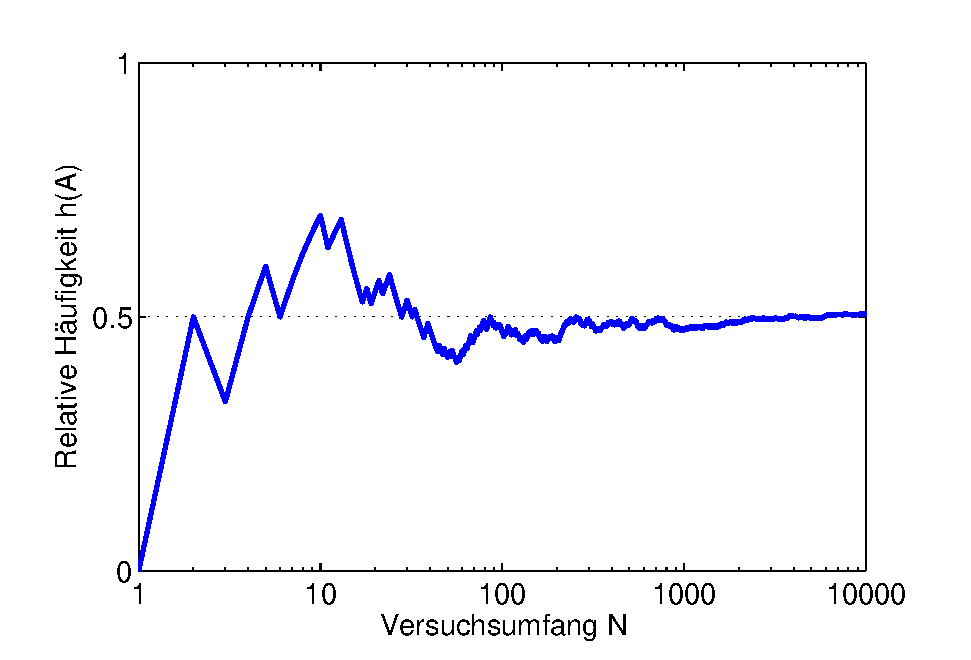
\includegraphics[width=0.8\textwidth]{Kapitel5/Bilder/image9}}
  \caption{Elektronischer Batteriesensor (Robert Bosch GmbH, Gesch\"{a}ftsbereich AE Automotive Electronics)}
  \label{fig:Batteriewiderstand1}
\end{figure}

\noindent Der Sensor wird mit einer Polklemme auf dem Batterie-Minus-Pol montiert. Die Verbindung zur Karosserie (Massekabel) erfolgt \"{u}ber einen Kabelschuh, der mit dem Batteriesensor verschraubt wird. \"{U}ber diesen Schraubkontakt k\"{o}nnen Str\"{o}me im Bereich von mehreren 100 A flie{\ss}en, sodass der \"{U}bergangswiderstand zwischen Sensor und Kabelschuh klein gehalten werden muss. Dieser Widerstand setzt sich aus dem Fremdschichtwiderstand, der durch immer vorhandene, d\"{u}nne Oxid- oder Sulfidschichten verursacht wird, und dem sogenannten Engewiderstand zusammen. Die Summe beider Widerst\"{a}nde darf einen maximalen Wert von R$_{E,MAX}$ von 100µ$\Omega$ nicht \"{u}berschreiten.\newline

\noindent Der Engewiderstand ergibt sich aus der Ber\"{u}hrfl\"{a}che des Batteriesensorkontaktes und des Kabelschuhs. Beide Partner sind nicht ideal eben und weisen eine Oberfl\"{a}chenrauhigkeit auf, die effektive Kontaktfl\"{a}che ist daher erheblich kleiner als die Grundfl\"{a}che der Kontakte. Der flie{\ss}ende Strom muss durch diese Engstellen flie{\ss}en. Daraus ergibt sich der Name Engewiderstand.

\noindent 
\begin{figure}[H]
  \centerline{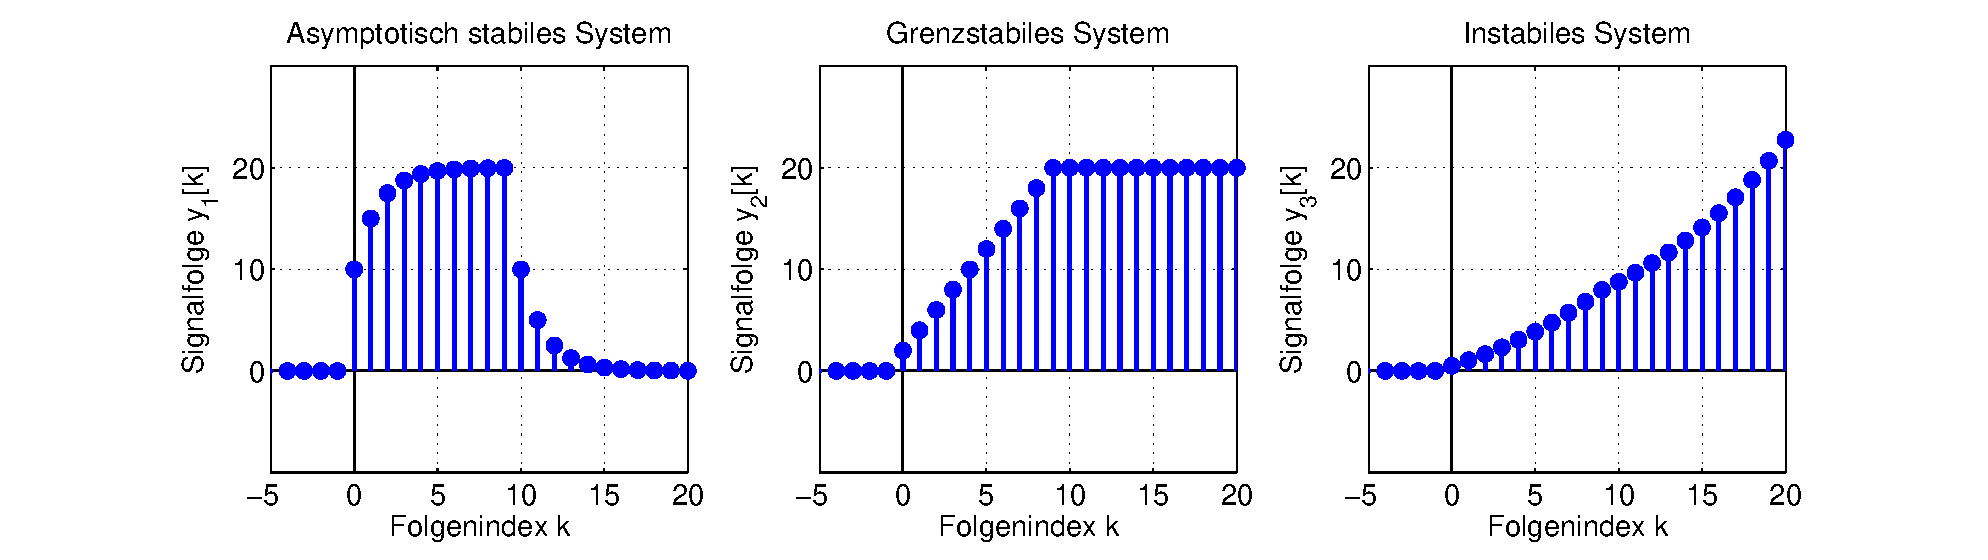
\includegraphics[width=0.8\textwidth]{Kapitel5/Bilder/image10}}
  \caption{Beschreibung der effektiven Kontaktfl\"{a}che eines Batteriesensors}
  \label{fig:Batteriewiderstand2}
\end{figure}

\noindent Der elektrische Kontakt besteht nur an wenigen, sehr kleinen Ber\"{u}hrfl\"{a}chen. Durch die Vorspannkraft F$_{V}$, die durch die Verschraubung aufgebracht wird, werden diese Kontaktstellen plastisch verformt, sodass sie an Gr\"{o}{\ss}e und Anzahl wachsen.\newline

\noindent Die mathematische Modellierung [Holm67, H\"{o}ft80] zeigt, dass im Fall der plastischen Verformung der Engewiderstand R$_{E}$ im Wesentlichen von der spezifischen Leitf\"{a}higkeit $\rhoup$, der Kontakth\"{a}rte H und der Vorspannkraft F$_{V}$ abh\"{a}ngt und durch die Gleichung

\begin{equation}\label{eq:fivehundredfiftynine}
R_{E} =\dfrac{\rho}{2} \cdot \sqrt{\dfrac{\pi \cdot H}{F_{V}}}
\end{equation}

\noindent beschrieben werden kann. Um die theoretische Berechnung des Engewiderstandes zu hinterfragen, wurden Musterteile des Batteriesensors aufgebaut, an denen der Engewiderstand gemessen wurde. Bild \ref{fig:Batteriesensor1} zeigt das Ergebnis der mathematischen Modellierung des Engewiderstandes und einer elektrischen Messung des Engewiderstandes an Neuteilen. Es zeigt sich, dass die theoretische Berechnung des Engewiderstandes f\"{u}r Vorspannkr\"{a}fte, die gr\"{o}{\ss}er als 1500 N sind, als konservative Absch\"{a}tzung f\"{u}r den Engewiderstand verwendet werden kann.

\noindent 
\begin{figure}[H]
  \centerline{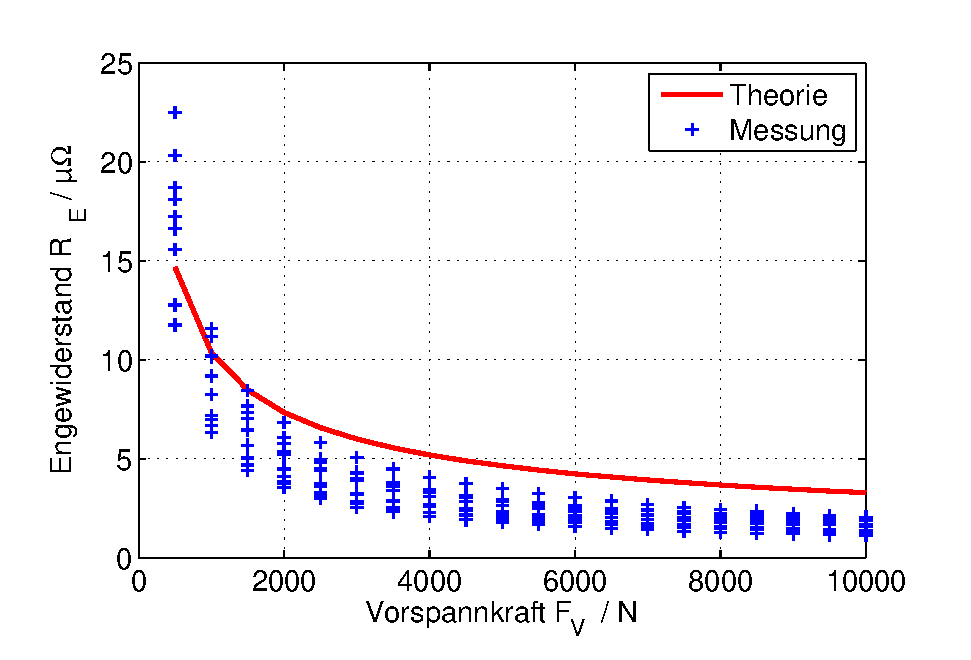
\includegraphics[width=0.5\textwidth]{Kapitel5/Bilder/image11}}
  \caption{Ergebnis einer mathematischen Modellierung des Engewiderstandes R$_{E}$und einer elektrischen Messung des Engewiderstandes R$_{E}$ an Neuteilen}
  \label{fig:Batteriesensor1}
\end{figure}

\noindent Neben der Vorspannkraft hat die Oberfl\"{a}chenbeschaffenheit einen starken Einfluss auf den Kontaktwiderstand. Deshalb wurde in zwei Szenarien analysiert, wie sich unterschiedliche Vorbehandlungen auf den Widerstandswert auswirken. Die Sensoren wurden zum einen in Standardverpackungen als Seefracht transportiert, um den Einfluss der Seeatmosph\"{a}re zu bewerten. Zum anderen durchliefen die Teile mehrfach eine L\"{o}teinrichtung mit anschlie{\ss}ender Abk\"{u}hlung in einer Industrieatmosph\"{a}re, sodass die Oberfl\"{a}che der Kontakte oxidierte. Bild \ref{fig:Batteriesensor2} stellt f\"{u}r beide Vorbehandlungen die Ergebnisse der Nachmessung und die mit Gleichung \eqref{eq:fivehundredfiftynine} berechneten Widerstandswerte dar.

\noindent 
\begin{figure}[H]
  \centerline{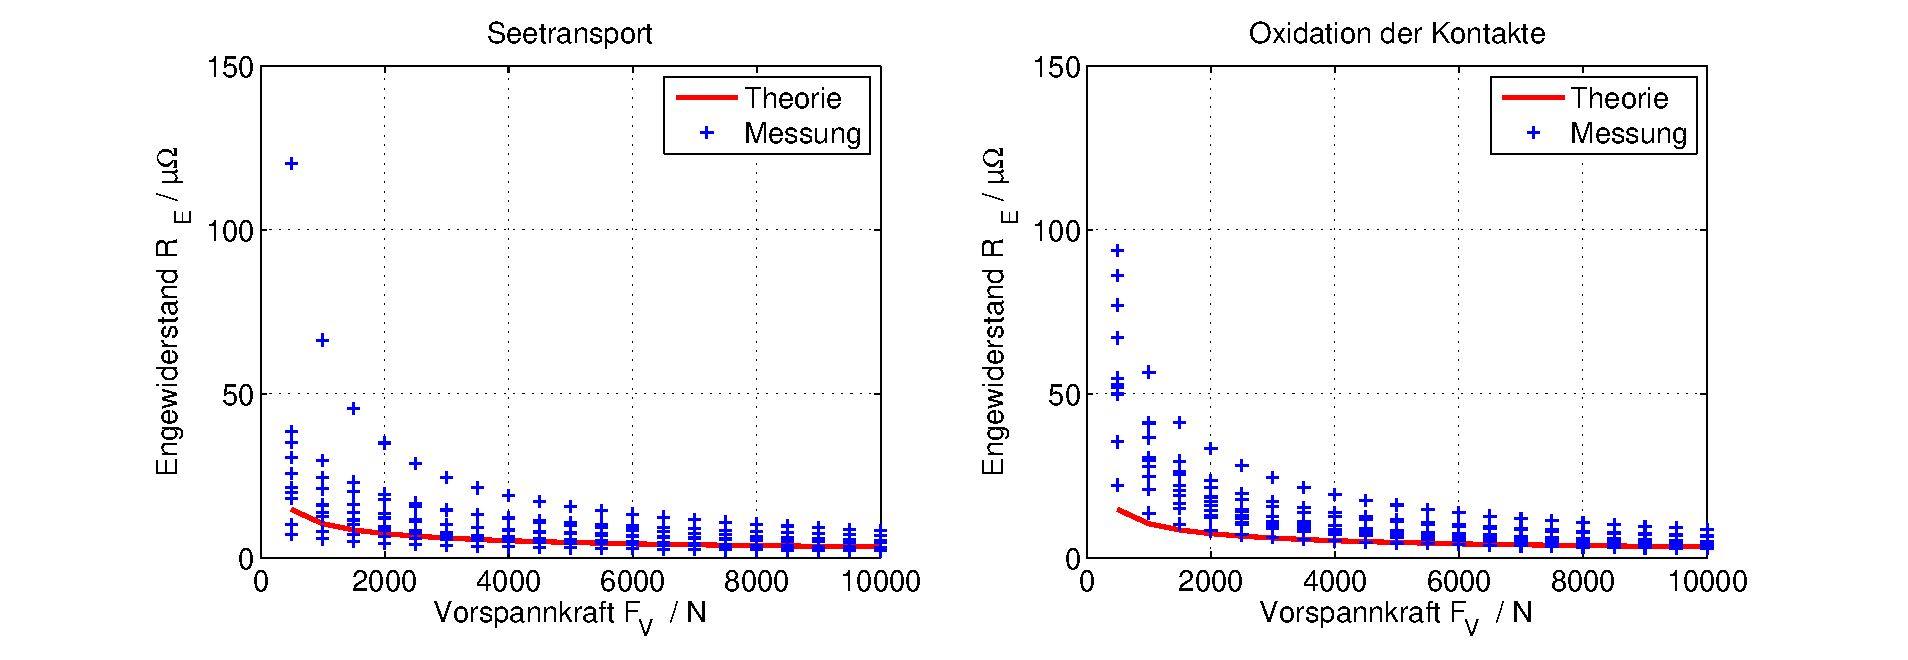
\includegraphics[width=1\textwidth]{Kapitel5/Bilder/image12}}
  \caption{Elektrische Messung des Kontaktwiderstandes nach Vorbehandlunga) Simulierter Seetransport der Shunt-Widerst\"{a}ndeb) Oxidierte Shunt-Widerst\"{a}nde}
  \label{fig:Batteriesensor2}
\end{figure}

\noindent Durch die Vorbehandlung steigt der Kontaktwiderstand erwartungsgem\"{a}{\ss} an, der st\"{a}rkste Anstieg wird bei Seetransport verzeichnet. Bei niedrigen Vorspannkr\"{a}ften steigt der Kontaktwiderstand gegen\"{u}ber der Messung bei Neuteilen um bis zu einem Faktor 10. \newline

\noindent F\"{u}r die Montage der Sensoren und die Auslegung der Schraubverbindung muss die Frage beantwortet werden, wie gro{\ss} die von der Verschraubung aufzubringende Vorspannkraft F$_{V}$ sein muss, damit der Widerstand unter der definierten Grenze von R$_{E,MAX}$ = 100 µ$\Omega$ bleibt. Hier wird vereinfachend davon ausgegangen, dass nur die beschriebenen Einfl\"{u}sse auf den Kontaktwiderstand auftreten und dass sich die Effekte nicht \"{u}berlagern. Die Sensoren d\"{u}rfen in diesem Beispiel au{\ss}erdem nur mit einer Wahrscheinlichkeit von 10 ppm einen Kontaktwiderstand oberhalb des definierten Grenzwertes R$_{E,MAX}$ aufweisen.\newline

\noindent F\"{u}r jede Kombination von Vorspannkraft und Vorbehandlung existieren 10 Stichprobenwerte. Sie sind in Tabelle 5.21 exemplarisch f\"{u}r die Vorbehandlung durch Oxidation und eine Vorspannkraft von 6000 N zusammengestellt.

\begin{table}[H]
\caption{Stichprobe von Messwerten des Kontaktwiderstandes bei Vorbehandlung durch Oxidation und einer Vorspannkraft von 6000 N}
\setlength{\fboxsep}{0pt}%
\colorbox{lightgray}{%
\arrayrulecolor{white}%
\begin{tabular}{| c | c | c | c | c | c | c | c | c | c | c |}
\hline

\parbox[c][0.28in][c]{0.5in}{\smallskip\centering\fontfamily{phv}\selectfont\textbf{Nr.}} &
\parbox[c][0.28in][c]{0.45in}{\centering\fontfamily{phv}\selectfont\textbf{1}} &
\parbox[c][0.28in][c]{0.45in}{\centering\fontfamily{phv}\selectfont\textbf{2}} &
\parbox[c][0.28in][c]{0.45in}{\centering\fontfamily{phv}\selectfont\textbf{3}} &
\parbox[c][0.28in][c]{0.45in}{\centering\fontfamily{phv}\selectfont\textbf{4}} &
\parbox[c][0.28in][c]{0.45in}{\centering\fontfamily{phv}\selectfont\textbf{5}} &
\parbox[c][0.28in][c]{0.45in}{\centering\fontfamily{phv}\selectfont\textbf{6}} &
\parbox[c][0.28in][c]{0.45in}{\centering\fontfamily{phv}\selectfont\textbf{7}} &
\parbox[c][0.28in][c]{0.45in}{\centering\fontfamily{phv}\selectfont\textbf{8}} &
\parbox[c][0.28in][c]{0.45in}{\centering\fontfamily{phv}\selectfont\textbf{9}} &
\parbox[c][0.28in][c]{0.45in}{\centering\fontfamily{phv}\selectfont\textbf{10}} \\ \hline

\parbox[c][0.35in][c]{0.5in}{\smallskip\centering\fontfamily{phv}\selectfont\textbf{R$_{E}$ / $\mu \Omega$}} &
\parbox[c][0.35in][c]{0.45in}{\centering\fontfamily{phv}\selectfont{3.984}} &
\parbox[c][0.35in][c]{0.45in}{\centering\fontfamily{phv}\selectfont{7.349}} &
\parbox[c][0.35in][c]{0.45in}{\centering\fontfamily{phv}\selectfont{6.451}} &
\parbox[c][0.35in][c]{0.45in}{\centering\fontfamily{phv}\selectfont{5.952}} &
\parbox[c][0.35in][c]{0.45in}{\centering\fontfamily{phv}\selectfont{7.076}} &
\parbox[c][0.35in][c]{0.45in}{\centering\fontfamily{phv}\selectfont{13.633}} &
\parbox[c][0.35in][c]{0.45in}{\centering\fontfamily{phv}\selectfont{10.065}} &
\parbox[c][0.35in][c]{0.45in}{\centering\fontfamily{phv}\selectfont{5.478}} &
\parbox[c][0.35in][c]{0.45in}{\centering\fontfamily{phv}\selectfont{9.529}} &
\parbox[c][0.35in][c]{0.45in}{\centering\fontfamily{phv}\selectfont{5.263}} \\ \hline

\end{tabular}%
}\bigskip
\label{tab:fivetwentyone}
\end{table}

\noindent Zur besseren \"{U}bersicht zeigt Bild \ref{fig:Batteriesensor3} die H\"{a}ufigkeitsverteilung und den Box-Plot der Stichprobe bei Vorbehandlung durch Seetransport und einer Vorspannkraft von 6000 N. Es wird von einer normalverteilten Grundgesamtheit ausgegangen. 

\noindent 
\begin{figure}[H]
  \centerline{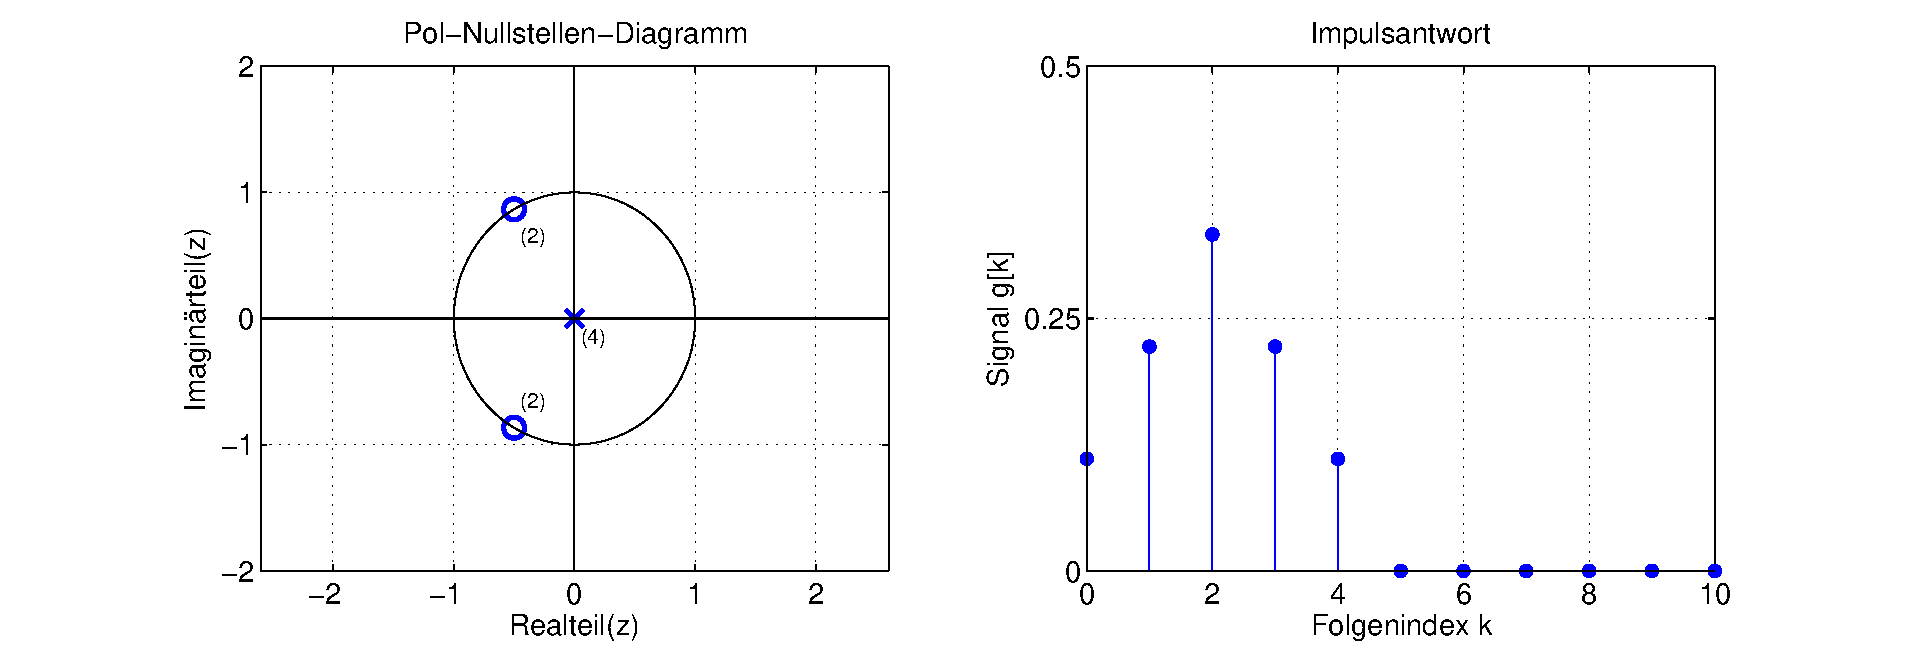
\includegraphics[width=1\textwidth]{Kapitel5/Bilder/image13}}
  \caption{Verteilungsfunktion und Box-Plot der Stichprobe bei Vorbehandlung durch Seetransport und einer Vorspannkraft von 6000 N}
  \label{fig:Batteriesensor3}
\end{figure}

\noindent Die Bestimmung der erforderlichen Vorspannkraft F$_{V}$ ergibt sich aus der Prognose zuk\"{u}nftiger Kontaktwiderst\"{a}nde. Bei der Prognose sind weder Mittelwert, noch Standardabweichung bekannt. Damit ergibt sich die obere Grenze des Engewiderstandes zu

\begin{equation}\label{eq:fivehundredsixty}
R_{E} \le \bar{R}_{E} +c_{2} \cdot s\cdot \sqrt{1+\dfrac{1}{N}}
\end{equation}

\noindent Dabei berechnet sich die Konstante c$_{2}$ \"{u}ber die inverse t-Verteilung mit N - 1 Freiheitsgraden und $\gamma$ = 10 ppm zu

\begin{equation}\label{eq:fivehundredsixtyone}
c_{2} =F^{-1} (\gamma)=8.1021
\end{equation}

\noindent F\"{u}r den vorliegenden Fall wurden f\"{u}r jede Vorbehandlungsart N = 10 Teile untersucht. Mit den dabei aufgenommenen Messwerten ergeben sich f\"{u}r die Neuteile, die Teile nach Seetransport und die Teile mit oxidierten Kontakten die in Bild 5.14 dargestellten oberen Grenzen des Prognosebereiches des Kontaktwiderstandes als Funktion der Vorspannkraft.

\noindent 
\begin{figure}[H]
  \centerline{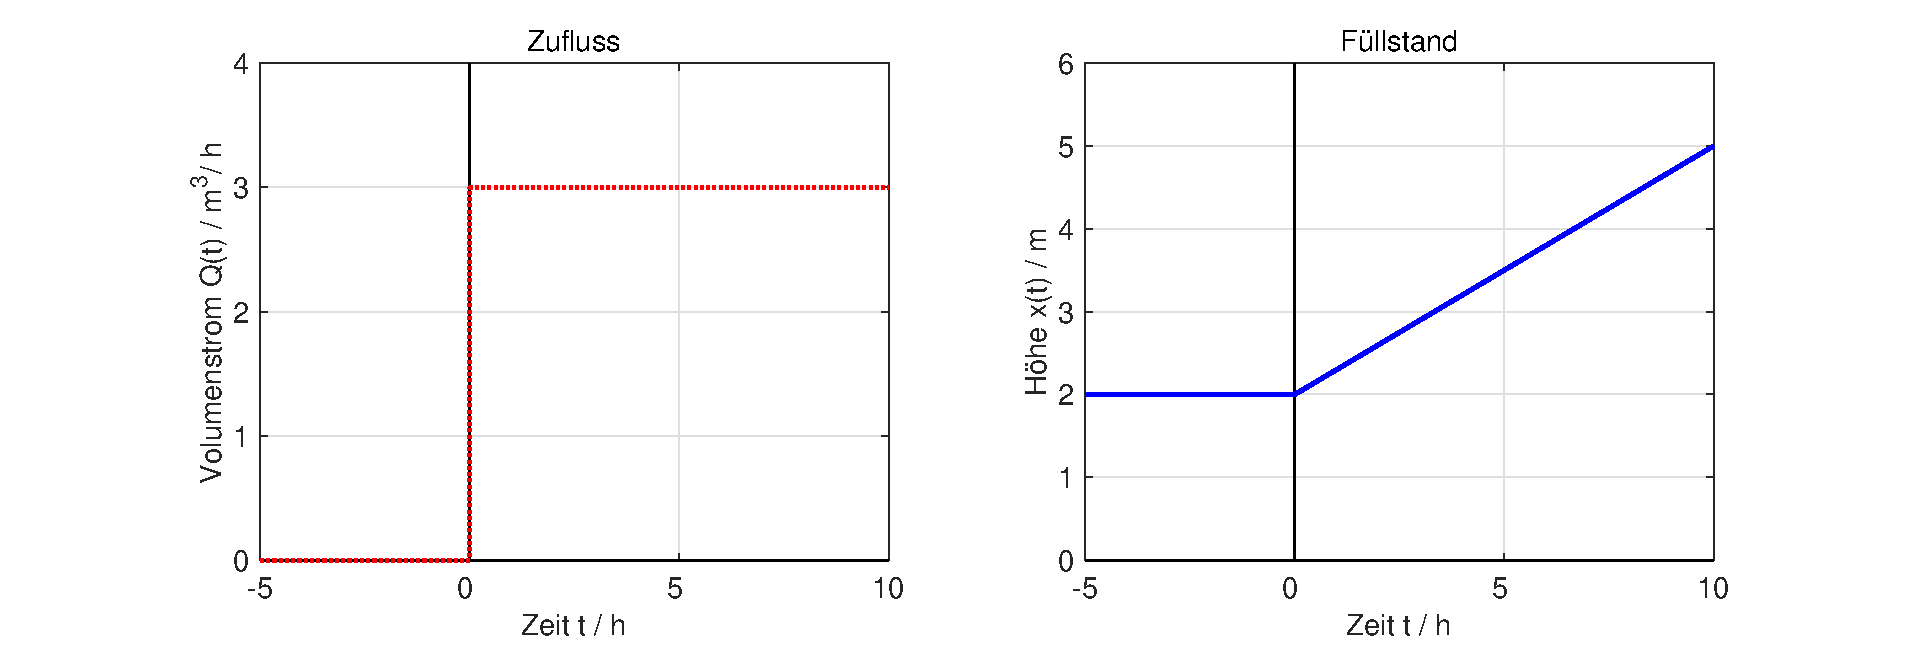
\includegraphics[width=0.5\textwidth]{Kapitel5/Bilder/image14}}
  \caption{Obere Grenze des Prognosebereiches von Kontaktwiderst\"{a}nden auf Basis von Erprobungsergebnissen(N = 10 Teile, $\gamma$ = 1 - 10 ppm)}
  \label{fig:Batteriesensor4}
\end{figure}

\noindent Es zeigt sich, dass die Kontaktwiderst\"{a}nde bei dem Seetransport zu den gr\"{o}{\ss}ten Prognosewerten f\"{u}hren. Nach diesen Erprobungsergebnissen und den beschriebenen Annahmen ist eine Vorspannkraft von F$_{V}$ = 1800 N erforderlich, um das spezifizierte Ziel von R$_{E}$ $\mathrm{<}$ 100 µ$\Omega$ mit einer Sicherheit von $\gamma$ = 1 - 10 ppm einzuhalten.\newline

\noindent Die Berechnung erfolgt in folgendem MATLAB-Programm. Es geht davon aus, dass die Daten als Matrix organisiert sind, bei denen jede Zeile eine Vorspannkraft und jede Spalte ein Stichprobenwert repr\"{a}sentiert.

\lstinputlisting[caption = {}]{Kapitel5/mat1.m}

\noindent Damit liegen die oberen Prognosegrenzen als Funktion der Vorspannkraft vor und k\"{o}nnen als Plot dargestellt werden.

\lstinputlisting[caption = {}]{Kapitel5/mat2.m}

\clearpage

\noindent Dasselbe Ergebnis ergibt sich bei der Umsetzung in Python:

\lstinputlisting[caption = {}]{Kapitel5/mat3.m}

\clearpage

\subsection{Literatur}

\begin{tabular}{|p{0.6in}|p{5.6in}|} \hline 
[Krey91] & Kreyszig, Erwin: Statistische Methoden und ihre Anwendungen\newline 4., unver\"{a}nderter Nachdruck der 7. Auflage\newline Vandenhoeck \& Ruprecht, G\"{o}ttingen, 1991 \\ \hline 
[Fahr06] & Fahrmeir, Ludwig; K\"{u}nstler, Rita; Pigeot, Iris; Tutz, Gerhard: Der Weg zur Datenanalyse\newline 6. Auflage\newline Springer Berlin Heidelberg New York, 2006 \\ \hline  

[Ross06] & Ross, M. Sheldon: Statistik f\"{u}r Ingenieure und Naturwissenschaftler\newline 3. Auflage\newline Spektrum Akademischer Verlag, M\"{u}nchen, 2006 \\ \hline 

[Papu01] & Papula, Lothar: Mathematik f\"{u}r Ingenieure und Naturwissenschaftler Band 3\newline 4., verbesserte Auflage\newline Vieweg Teubner, Braunschweig / Wiesbaden, 2008 \\ \hline 

[Holm67] & Holm, Ragnar: Electric Contacts - Theory and Application\newline Fourth completely rewritten edition\newline Springer-Verlag Berlin/Heidelberg/New York 1967 \\ \hline 

[H\"{o}ft80] & H\"{o}ft, Herbert: Elektrische Kontakte - Ausgew\"{a}hlte Beitr\"{a}ge\newline 1. Auflage\newline Akademie-Verlag Berlin 1980 \\ \hline 
\end{tabular}
